% Generated from SWEVO_manuscript.tex. Edit modular sources, then regenerate.
% Canonical modular manuscript. Edit its section files; regenerate the full file with analysis/flatten_manuscript.py.
% begin manuscript_preamble.tex
% Shared preamble; cross references refreshed by analysis/build_swevo.sh.
\documentclass[preprint,12pt,number]{elsarticle}
\usepackage{lmodern}
% numbered references [1], [2], ... (natbib numbers; manual thebibliography in optA/swevo_back.tex);
% sort&compress gives [1-3] ranges as the cite package does in the MPCE version
\biboptions{sort&compress}
% A4 text block slightly larger than the elsarticle preprint default, so that the tallest generated table
% (analysis/mpce_tab_ablation.tex) fits on a page; \emergencystretch avoids overfull lines in the contribution list
\usepackage[a4paper,margin=2.5cm]{geometry}
\setlength{\emergencystretch}{1.5em}
% elsarticle 3.3 puts a stray space after the title-page footer box ("Preprint submitted to ..."), which gives an
% Overfull \hbox of about 2.6pt on page 1 in any document; absorb it (layout unchanged)
\makeatletter
\let\swevo@pprintTitle\ps@pprintTitle
\def\ps@pprintTitle{\swevo@pprintTitle\let\swevo@oddfoot\@oddfoot
  \def\@oddfoot{\hbox to\textwidth{\swevo@oddfoot\hss}}\let\@evenfoot\@oddfoot}
\makeatother
% continuous line numbers for review, starting after the title page (switched on right after \end{frontmatter};
% numbering the elsarticle title page itself pushes its footnotes into the footer)
\usepackage{lineno}
\usepackage{etoolbox}
\AfterEndEnvironment{frontmatter}{\linenumbers}
\usepackage{amsmath,amssymb,amsfonts}
\usepackage{algorithm}
\usepackage{algpseudocode}
\usepackage{booktabs}
\usepackage{graphicx}
\usepackage{textcomp}
\usepackage{multirow}
\usepackage{array}
\usepackage{xcolor}
\usepackage{url}
% Numbers of the supplementary-material items cited in this file (Tables S*, Figs. S*, Sections S*), copied from
% SWEVO_supplement.aux, so that this file compiles on its own (no xr package / xref folder needed).
% If the numbering of the supplement changes, recompile the supplement and update these lines.
% begin xref/supplement_labels.tex
\makeatletter
\newlabel{S-sec:S-protocol}{{S1}{1}{}{}{}}
\newlabel{S-sec:S-impl}{{S1}{1}{}{}{}}
\newlabel{S-sec:S-wind}{{S1.1}{1}{}{}{}}
\newlabel{S-tab:S-wind}{{S1}{1}{}{}{}}
\newlabel{S-sec:S-ssa-alg}{{S1.2}{2}{}{}{}}
\newlabel{S-alg:S-ssa}{{S1}{2}{}{}{}}
\newlabel{S-sec:S-stats}{{S1.3}{2}{}{}{}}
\newlabel{S-sec:S-iter}{{S1.4}{2}{}{}{}}
\newlabel{S-sec:S-slsqp}{{S1.5}{3}{}{}{}}
\newlabel{S-sec:S-feasinit-impl}{{S1.6}{3}{}{}{}}
\newlabel{S-eq:S-packing}{{S1}{3}{}{}{}}
\newlabel{S-alg:S-feasinit}{{S2}{3}{}{}{}}
\newlabel{S-sec:S-hrmodel}{{S1.7}{3}{}{}{}}
\newlabel{S-sec:S-tol}{{S1.8}{4}{}{}{}}
\newlabel{S-sec:S-tables}{{S2}{4}{}{}{}}
\newlabel{S-sec:S-psosetting}{{S2.1}{4}{}{}{}}
\newlabel{S-tab:baseline-cases}{{S2}{5}{}{}{}}
\newlabel{S-sec:S-csweep}{{S2.2}{6}{}{}{}}
\newlabel{S-tab:S-csweep}{{S3}{6}{}{}{}}
\newlabel{S-sec:S-percase}{{S2.3}{6}{}{}{}}
\newlabel{S-tab:res-1-500}{{S4}{6}{}{}{}}
\newlabel{S-tab:res-1-750}{{S5}{7}{}{}{}}
\newlabel{S-tab:res-1-1000}{{S6}{7}{}{}{}}
\newlabel{S-tab:res-2-500}{{S7}{7}{}{}{}}
\newlabel{S-tab:res-2-750}{{S8}{7}{}{}{}}
\newlabel{S-tab:res-2-1000}{{S9}{8}{}{}{}}
\newlabel{S-sec:S-caselevel}{{S2.4}{8}{}{}{}}
\newlabel{S-tab:friedman68-full}{{S10}{8}{}{}{}}
\newlabel{S-tab:coords}{{S11}{8}{}{}{}}
\newlabel{S-sec:S-figs}{{S2.5}{8}{}{}{}}
\newlabel{S-fig:S-ranks}{{S1}{9}{}{}{}}
\newlabel{S-fig:S-conv-max}{{S2}{9}{}{}{}}
\newlabel{S-fig:S-conv-mid}{{S3}{10}{}{}{}}
\newlabel{S-fig:S-box-max}{{S4}{10}{}{}{}}
\newlabel{S-fig:S-box-mid}{{S5}{11}{}{}{}}
\newlabel{S-fig:S-feas}{{S6}{11}{}{}{}}
\newlabel{S-fig:S-layouts}{{S7}{12}{}{}{}}
\newlabel{S-sec:S-ablation}{{S3}{13}{}{}{}}
\newlabel{S-tab:split}{{S12}{14}{}{}{}}
\newlabel{S-tab:ablation-cases}{{S13}{14}{}{}{}}
\newlabel{S-tab:switch}{{S14}{15}{}{}{}}
\newlabel{S-tab:equivalence}{{S15}{16}{}{}{}}
\newlabel{S-tab:split-cases}{{S16}{16}{}{}{}}
\newlabel{S-sec:S-inference}{{S3.1}{17}{}{}{}}
\newlabel{S-tab:X-equiv-levels}{{S17}{18}{}{}{}}
\newlabel{S-tab:X-threshold}{{S18}{18}{}{}{}}
\newlabel{S-tab:X-threshold-controls}{{S19}{19}{}{}{}}
\newlabel{S-tab:X-cluster}{{S20}{19}{}{}{}}
\newlabel{S-tab:X-loco}{{S21}{20}{}{}{}}
\newlabel{S-tab:X-cluster-split}{{S22}{20}{}{}{}}
\newlabel{S-tab:X-multiplicity}{{S23}{21}{}{}{}}
\newlabel{S-tab:X-subgroup}{{S24}{21}{}{}{}}
\newlabel{S-tab:X-energy}{{S25}{22}{}{}{}}
\newlabel{S-tab:X-modelshift}{{S26}{22}{}{}{}}
\newlabel{S-tab:X-bayes}{{S27}{22}{}{}{}}
\newlabel{S-tab:X-heterogeneity}{{S28}{23}{}{}{}}
\newlabel{S-tab:X-beyond}{{S29}{23}{}{}{}}
\newlabel{S-tab:X-hl}{{S30}{24}{}{}{}}
\newlabel{S-tab:X-mcnemar}{{S31}{24}{}{}{}}
\newlabel{S-sec:S-beyond}{{S4}{24}{}{}{}}
\newlabel{S-sec:S-feasbudget}{{S4.1}{24}{}{}{}}
\newlabel{S-tab:feasinit-cases}{{S32}{25}{}{}{}}
\newlabel{S-tab:budget-cases}{{S33}{26}{}{}{}}
\newlabel{S-sec:S-hr16}{{S4.2}{27}{}{}{}}
\newlabel{S-tab:hr-site-full}{{S34}{27}{}{}{}}
\newlabel{S-fig:S-hr16}{{S8}{27}{}{}{}}
\newlabel{S-sec:S-iea37}{{S4.3}{28}{}{}{}}
\newlabel{S-tab:iea37-detail}{{S35}{28}{}{}{}}
\newlabel{S-tab:iea37-pub}{{S36}{28}{}{}{}}
\newlabel{S-fig:S-iea37-conv}{{S9}{29}{}{}{}}
\newlabel{S-fig:S-layouts-sites}{{S10}{29}{}{}{}}
\newlabel{S-sec:S-cost}{{S4.4}{29}{}{}{}}
\newlabel{S-tab:cost}{{S37}{29}{}{}{}}
\newlabel{S-sec:S-robust}{{S5}{30}{}{}{}}
\newlabel{S-sec:S-gauss}{{S5.1}{30}{}{}{}}
\newlabel{S-eq:S-gauss}{{S2}{30}{}{}{}}
\newlabel{S-sec:S-robust-tables}{{S5.2}{30}{}{}{}}
\newlabel{S-tab:robust}{{S38}{30}{}{}{}}
\newlabel{S-tab:capacity}{{S39}{30}{}{}{}}
\newlabel{S-tab:spacing-authors}{{S40}{31}{}{}{}}
\newlabel{S-sec:S-direction}{{S5.3}{31}{}{}{}}
\newlabel{S-tab:F-bench}{{S41}{32}{}{}{}}
\newlabel{S-tab:F-equiv}{{S42}{32}{}{}{}}
\newlabel{S-tab:F-abl}{{S43}{33}{}{}{}}
\newlabel{S-tab:F-hr}{{S44}{33}{}{}{}}
\newlabel{S-tab:F-hrpair}{{S45}{34}{}{}{}}
\newlabel{S-tab:F-pywake}{{S46}{34}{}{}{}}
\newlabel{S-tab:F-iea}{{S47}{35}{}{}{}}
\newlabel{S-tab:F-iea-gap}{{S48}{35}{}{}{}}
\newlabel{S-sec:S-theory}{{S6}{36}{}{}{}}
\newlabel{S-sec:S-th-pso}{{S6.1}{36}{}{}{}}
\newlabel{S-eq:S-th-upd}{{S3}{36}{}{}{}}
\newlabel{S-eq:S-th-rec}{{S4}{36}{}{}{}}
\newlabel{S-prop:S-pso-stability}{{S1}{36}{}{}{}}
\newlabel{S-eq:S-th-o1}{{S5}{36}{}{}{}}
\newlabel{S-eq:S-th-o2}{{S6}{36}{}{}{}}
\newlabel{S-eq:S-th-vinf}{{S7}{36}{}{}{}}
\newlabel{S-tab:S-th-settings}{{S49}{37}{}{}{}}
\newlabel{S-prop:S-settings}{{S2}{37}{}{}{}}
\newlabel{S-lem:S-clip}{{S3}{38}{}{}{}}
\newlabel{S-sec:S-th-budget}{{S6.2}{38}{}{}{}}
\newlabel{S-prop:S-prefix}{{S4}{38}{}{}{}}
\newlabel{S-eq:S-th-lens}{{S8}{38}{}{}{}}
\newlabel{S-tab:S-th-box}{{S50}{39}{}{}{}}
\newlabel{S-sec:S-th-feas}{{S6.3}{39}{}{}{}}
\newlabel{S-lem:S-feas-improve}{{S5}{39}{}{}{}}
\newlabel{S-prop:S-frozen}{{S6}{39}{}{}{}}
\newlabel{S-prop:S-de}{{S7}{40}{}{}{}}
\newlabel{S-sec:S-th-equiv}{{S6.4}{40}{}{}{}}
\newlabel{S-lem:S-tost-ci}{{S8}{40}{}{}{}}
\newlabel{S-sec:S-th-vns}{{S6.5}{41}{}{}{}}
\newlabel{S-prop:S-ls}{{S9}{41}{}{}{}}
\newlabel{S-eq:S-th-ls}{{S9}{41}{}{}{}}
\newlabel{S-fig:D-psodyn}{{S11}{42}{}{}{}}
\newlabel{S-tab:D-psodyn}{{S51}{42}{}{}{}}
\newlabel{S-sec:S-diag}{{S7}{42}{}{}{}}
\newlabel{S-sec:S-diag-pso}{{S7.1}{42}{}{}{}}
\newlabel{S-tab:D-vns}{{S52}{43}{}{}{}}
\newlabel{S-tab:D-feasstart}{{S53}{43}{}{}{}}
\newlabel{S-tab:D-rsreplay}{{S54}{44}{}{}{}}
\newlabel{S-sec:S-diag-vns}{{S7.2}{44}{}{}{}}
\newlabel{S-sec:S-diag-feas}{{S7.3}{44}{}{}{}}
\newlabel{S-sec:S-diag-rs}{{S7.4}{45}{}{}{}}
\newlabel{S-sec:S-literature}{{S8}{45}{}{}{}}
\newlabel{S-sec:S-repro}{{S9}{45}{}{}{}}
\newlabel{S-tab:S-repro}{{S55}{46}{}{}{}}
\newlabel{S-tab:provenance}{{S56}{47}{}{}{}}
\newlabel{S-sec:S-xp-lap}{{S10}{48}{}{}{}}
\newlabel{S-sec:S-xp-lap-abl}{{S10.1}{48}{}{}{}}
\newlabel{S-tab:S-xp-laplace}{{S57}{49}{}{}{}}
\newlabel{S-sec:S-xp-ga}{{S10.2}{49}{}{}{}}
\newlabel{S-tab:S-xp-ga}{{S58}{50}{}{}{}}
\newlabel{S-tab:S-xp-ga-hr}{{S59}{50}{}{}{}}
\newlabel{S-tab:S-xp-ga-iea}{{S60}{50}{}{}{}}
\newlabel{S-sec:S-xp-spacing}{{S10.3}{51}{}{}{}}
\newlabel{S-sec:S-xp-grad}{{S10.4}{51}{}{}{}}
\newlabel{S-tab:S-xp-spacing-rank}{{S61}{52}{}{}{}}
\newlabel{S-tab:S-xp-spacing}{{S62}{52}{}{}{}}
\newlabel{S-sec:S-xp-site}{{S10.5}{53}{}{}{}}
\newlabel{S-tab:S-xp-grad}{{S63}{54}{}{}{}}
\newlabel{S-tab:S-xp-grad-calls}{{S64}{54}{}{}{}}
\newlabel{S-tab:S-xp-site}{{S65}{56}{}{}{}}
\newlabel{S-sec:S-sa}{{S11}{56}{}{}{}}
\newlabel{S-sec:S-sa-allrun}{{S11.1}{56}{}{}{}}
\newlabel{S-sec:S-sa-dep}{{S11.2}{56}{}{}{}}
\newlabel{S-tab:S-sa-allrun}{{S66}{57}{}{}{}}
\newlabel{S-tab:S-sa-dep-bench}{{S67}{58}{}{}{}}
\newlabel{S-sec:S-sa-tost}{{S11.3}{58}{}{}{}}
\newlabel{S-tab:S-sa-dep-studies}{{S68}{59}{}{}{}}
\newlabel{S-tab:S-sa-tostaudit}{{S69}{60}{}{}{}}
\newlabel{S-sec:S-sa-seeds}{{S11.4}{60}{}{}{}}
\newlabel{S-sec:S-sa-imput}{{S11.5}{60}{}{}{}}
\newlabel{S-sec:S-sa-eqclus}{{S11.6}{60}{}{}{}}
\newlabel{S-tab:S-sa-syncseed}{{S70}{61}{}{}{}}
\newlabel{S-tab:S-sa-imputation}{{S71}{61}{}{}{}}
\newlabel{S-tab:S-sa-eqclus}{{S72}{62}{}{}{}}
\newlabel{S-tab:S-eqclus}{{S72}{62}{}{}{}}
\newlabel{S-sec:S-sa-pools}{{S11.7}{62}{}{}{}}
\newlabel{S-tab:S-sa-hr-pool}{{S73}{62}{}{}{}}
\newlabel{S-tab:S-sa-iea-pool}{{S74}{63}{}{}{}}
\newlabel{S-sec:S-sa-eval}{{S11.8}{63}{}{}{}}
\newlabel{S-tab:S-sa-hr-eval}{{S75}{64}{}{}{}}
\newlabel{S-tab:S-sa-lg-eval}{{S76}{64}{}{}{}}
\newlabel{S-sec:S-sa-time}{{S11.9}{65}{}{}{}}
\newlabel{S-tab:S-sa-time}{{S77}{65}{}{}{}}
\newlabel{S-tab:S-sa-time-sites}{{S78}{65}{}{}{}}
\newlabel{S-sec:S-sa-constraint}{{S11.10}{66}{}{}{}}
\newlabel{S-tab:S-sa-constraint}{{S79}{66}{}{}{}}
\newlabel{S-tab:S-sa-constraint-cases}{{S80}{67}{}{}{}}
\newlabel{S-sec:S-sa-fine}{{S11.11}{67}{}{}{}}
\newlabel{S-tab:S-sa-fine}{{S81}{68}{}{}{}}
\newlabel{S-sec:S-sa-precision}{{S11.12}{68}{}{}{}}
\newlabel{S-tab:S-sa-precision}{{S82}{69}{}{}{}}
\newlabel{S-sec:S-sa-feasbounds}{{S11.13}{70}{}{}{}}
\newlabel{S-tab:S-sa-feasbounds}{{S83}{71}{}{}{}}
\newlabel{S-tab:S-sa-feasworst}{{S84}{71}{}{}{}}
\newlabel{S-tab:S-sa-roundtransfer}{{S85}{72}{}{}{}}
\newlabel{S-sec:S-archive}{{S12}{73}{}{}{}}
\newlabel{S-sec:archive-precision}{{S12.2}{73}{}{}{}}
\newlabel{S-tab:archive-reliability}{{S86}{74}{}{}{}}
\newlabel{S-tab:archive-paired}{{S87}{74}{}{}{}}
\newlabel{S-sec:S-addl}{{S12.4}{75}{}{}{}}
\newlabel{S-tab:S-allrun-spacing}{{S88}{75}{}{}{}}
\newlabel{S-tab:S-time}{{S89}{75}{}{}{}}
\makeatother

% end xref/supplement_labels.tex



\journal{Swarm and Evolutionary Computation}

% Visible placeholder for author information and for numbers whose runs are still pending
% (an empty argument, used in table cells, prints just [TBD])
\newcommand{\TBD}[1]{\textcolor{red}{[TBD\ifx\relax#1\relax\else: #1\fi]}}
% All numbers (formerly \N... macros from analysis/mpce_numbers*.tex) are written directly in the text below.
% Figure from the analysis pipeline; a framed placeholder is printed while the file does not exist yet.
% #1 width, #2 file (with extension), #3 placeholder height
\newcommand{\pipefig}[3]{\IfFileExists{#2}{\includegraphics[width=#1]{#2}}%
{\fbox{\parbox[c][#3][c]{\dimexpr#1-2\fboxsep-2\fboxrule\relax}{\centering\TBD{figure {\ttfamily\detokenize{#2}} not yet generated}}}}}
% Extended SWEVO version: theorem environments and placement of generated tables by label
\usepackage{amsthm}
\usepackage{environ}
\newtheorem{lemma}{Lemma}\newtheorem{definition}{Definition}\newtheorem{remark}{Remark}
% >>>>> begin optA/sw/capture.tex
% Capture of generated supplementary tables so that the SWEVO main text can place some of them (\SuppTable{<label>}).
% Copied from SWEVO_supplement.tex (same macro names; no numbering changes).
\makeatletter
\newcount\supp@n
\def\supp@labels{}
\long\def\supp@getlabel#1\label#2#3\supp@stop{\def\supp@thislabel{#2}}
\newcommand{\supp@store}{%
  \global\advance\supp@n\@ne
  \expandafter\supp@getlabel\BODY\label{supp-unlabelled-\the\supp@n}\supp@stop
  \expandafter\global\expandafter\let\csname supp@body@\supp@thislabel\endcsname\BODY
  \xdef\supp@labels{\unexpanded\expandafter{\supp@labels}\noexpand\do{\supp@thislabel}}}
\newcommand{\CaptureSuppTables}[1]{\begingroup
  \RenewEnviron{table}[1][]{\supp@store}\RenewEnviron{table*}[1][]{\supp@store}%
  \input{#1}\endgroup}
\newcommand{\SuppTable}[1]{%
  \@ifundefined{supp@body@#1}{\par\noindent\TBD{generated table \detokenize{#1} not found}\par}{%
    \@ifundefined{supp@used@#1}{\global\@namedef{supp@used@#1}{}%
      \begin{table}[!htbp]\@nameuse{supp@body@#1}\end{table}}{}}}
\newcommand{\SuppTableOpt}[1]{\@ifundefined{supp@body@#1}{}{\SuppTable{#1}}}
\newcommand{\IfSuppTable}[3]{\@ifundefined{supp@body@#1}{#3}{#2}}
\newcommand{\SuppOmit}[1]{\global\@namedef{supp@used@#1}{}}
% \SuppTableNote{<label>}{<text>}: append a note below a captured table (inside its float); no-op if absent
\newcommand{\SuppTableNote}[2]{\@ifundefined{supp@body@#1}{}{%
  \expandafter\g@addto@macro\csname supp@body@#1\endcsname{\par\smallskip{\footnotesize\raggedright #2\par}}}}
\newif\ifsupp@left
\newcommand{\IfSuppTablesLeft}[1]{\global\supp@leftfalse
  \def\do##1{\@ifundefined{supp@used@##1}{\global\supp@lefttrue}{}}\supp@labels
  \ifsupp@left #1\fi}
\newcommand{\SuppRemainingTables}{\def\do##1{\SuppTable{##1}}\supp@labels}
% \SuppTableAddLabel{<label>}{<alias>}: give a captured table a second label (e.g. the name under which a table moved
% from the main text refers to it); no-op if the table is absent
\newcommand{\SuppTableAddLabel}[2]{\@ifundefined{supp@body@#1}{}{%
  \expandafter\g@addto@macro\csname supp@body@#1\endcsname{\label{#2}}}}
\makeatother

% <<<<< end optA/sw/capture.tex
% [flattened: removed \CaptureSuppTables{analysis/mpce_supplementary.tex}]
% Proposition environment used in optA/04_methods.tex (which also defines it, guarded, for the IEEEtran version)
\makeatletter\@ifundefined{proposition}{\newtheorem{proposition}{Proposition}}{}\makeatother



% end manuscript_preamble.tex

\begin{document}
% begin optA/swevo_front.tex
% Front matter of SWEVO_manuscript.tex (elsarticle), from optA/01_front.tex (the IEEEtran version for MPCE).
% Authors, affiliations and e-mail addresses as in the \thanks lines of optA/01_front.tex. The funding statement
% of the MPCE version is in the back matter (optA/swevo_back.tex); highlights are a separate file (SWEVO_highlights.txt).
\begin{frontmatter}

\title{Baseline Configuration and Random-Sampling Controls in Metaheuristic Comparisons for Wind Farm Layout Optimization}

\author[iilm]{Prince Solanki\corref{cor1}\fnref{fnprev}}
\ead{prince@ma.iitr.ac.in}
\ead{prince@iilm.edu}
\cortext[cor1]{Corresponding author.}
\fntext[fnprev]{Previously with the Department of Mathematics, Indian Institute of Technology Roorkee, Roorkee, India.}

\author[bennettcse]{Pulkit Dwivedi}
\ead{pdwivedi19900@gmail.com}
\ead{pulkit.dwivedi@bennett.edu.in}

\author[amity]{Vanita Garg}
\ead{vanitagarg16@gmail.com}

\author[sjtu,bennettmath]{Vinay Shukla}
\ead{vinayshukla4321@gmail.com}
\ead{vnshukla01@sjtu.edu.cn}

\affiliation[iilm]{organization={Department of Mathematics, School of Computer Science \& Engineering, IILM University},
            city={Gurugram},
            state={Haryana},
            country={India}}
\affiliation[bennettcse]{organization={Department of Computer Science and Engineering, Bennett University},
            city={Greater Noida},
            state={Uttar Pradesh},
            country={India}}
\affiliation[amity]{organization={Amity University},
            city={Noida},
            state={Uttar Pradesh},
            country={India}}
\affiliation[sjtu]{organization={School of Mathematical Sciences, Shanghai Jiao Tong University},
            city={Shanghai},
            postcode={200240},
            country={China}}
\affiliation[bennettmath]{organization={Department of Mathematics, School of Computer Science Engineering and Technology, Bennett University},
            city={Greater Noida},
            state={Uttar Pradesh},
            country={India}}

% Abstract: 209 words (rule: whitespace-separated tokens of the source after replacing ~ by a space, each inline formula $...$ counted as one word; 206 raw whitespace tokens of the source; PDF-text token count to be re-measured after compilation; SWEVO limit 250), no citations.
% CHECK (manual, 2026-10-04): direct 1-deg optimization, 8 cases, seeds 31-60: PSO-VNS first (rank 1.12), PSO-VNS - PSO -0.194 pp (analysis/rev3_fine.json, tab:S-sa-fine); IEA37 36 turbines: GA first among gradient-free methods, exact-gradient methods first overall (tab:S-sa-iea-pool);
% GA best on Horns Rev 1 at 30,030 also re-evaluated at 1 deg (+0.48 GWh/yr) and with PyWake NOJ (+0.43) (analysis/rev3_sites.json, tab:S-sa-hr-eval); constraint handling
% (analysis/rev3_constraint.json, tab:S-sa-constraint): 6 cases x 5 methods; Deb + box clipping changes the run-level order, projection keeps it and the conditional PSO-VNS - PSO dL -0.095 pp [-0.162, -0.037], PSO-VNS vs PSO all-run 0.561 ns
\begin{abstract}
We show how baseline configuration, random-sampling controls and the treatment of unsuccessful runs change comparisons of wind farm layout optimizers on the discretized Kusiak--Song benchmark (68 cases, 30 paired seeds, 6,030 evaluations). The PSO setting $w=0.7$, $c_1=c_2=2$, variance-unstable under stagnation, puts PSO behind salp-swarm hybrids; Clerc--Kennedy constriction puts it ahead. Against equal-cost disc sampling, an SSA first phase gains at most 0.05 percentage points (pp) of wake loss at $4D$ and $5D$ spacing, not at $6D$; against square sampling it appears to help. PSO followed by variable neighborhood search (PSO-VNS) ranks first; on this fixed benchmark its mean advantage over well-configured PSO lies within a post hoc $\pm0.05$~pp margin (not over scenario clusters), but reaches 0.19~pp when optimizing with 1$^\circ$ direction bins (eight cases). PSO-VNS reaches feasibility more often than PSO on two measured-wind blocks; conditional-quality rankings can miss the most reliable method. A real-coded genetic algorithm leads at the larger budget on Horns Rev~1 and among gradient-free methods with 36 IEA37 turbines; SLSQP with exact gradients, reported-feasible in all runs, beats every metaheuristic on IEA37 at equal charged budget. In a constraint-handling study (six cases, five methods), Deb's rules with box clipping change the ranking. Conclusions concern the tested implementations and models, not universal superiority.
\end{abstract}

% Graphical abstract (elsarticle 3.3: typeset by \maketitle on a separate page before the title page;
% figure from analysis/make_graphical_abstract.py, also submitted as a separate file)
\begin{graphicalabstract}
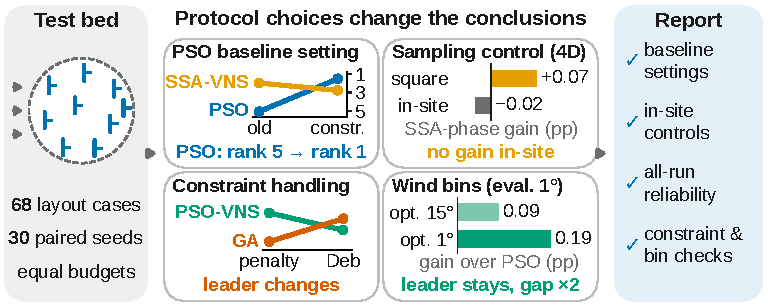
\includegraphics[width=\textwidth]{figures_final/graphical_abstract.pdf}
\end{graphicalabstract}

\begin{keyword}
Benchmarking \sep equivalence testing \sep particle swarm optimization \sep random-sampling control \sep constraint handling \sep wake effect \sep wind farm layout optimization
\end{keyword}

\end{frontmatter}

% Nomenclature (IEEEdescription in the MPCE version): compact two-column table after the front matter
\section*{Nomenclature}
\noindent
\begin{tabular}{@{}>{$}l<{$}@{\quad}l@{}}
B & Budget (number of evaluations)\\
C_T,\ K & Thrust coefficient; Jensen wake-spreading constant\\
D,\ R & Rotor diameter and rotor radius ($D=2R$)\\
E_{\rm ideal} & Wake-free benchmark objective of one turbine\\
F_p & Penalized wake loss (minimized)\\
\ell_{\min} & Minimum spacing between turbines\\
N,\ N_p & Number of turbines; population size\\
N_\theta,\ N_s & Numbers of wind-direction and wind-speed bins\\
r & Farm radius\\
w,\ c_1,\ c_2 & Inertia weight and acceleration coefficients of PSO\\
\mathbf X & Layout vector $(x_1,y_1,\ldots,x_N,y_N)$\\
\theta & Wind direction (blowing towards, CCW from east)\\
\omega & Fraction of the budget given to Phase~1
\end{tabular}

% end optA/swevo_front.tex

% begin optA/sw/02_intro.tex
\section{Introduction}
\label{sec:intro}

The positions of the turbines in a wind farm are fixed at the planning stage and determine, for its lifetime, how much of the available wind energy it converts. An upstream turbine leaves behind a wake of slower and more turbulent air that reduces the power of the turbines downstream, so the layout sets the wake loss and thereby the gross energy yield, and shapes the collector system and grid connection~\cite{Srikakulapu2018,Hou2019}. As the wake loss is a share of the wake-free energy, a difference of a few tenths of a percentage point is, within a given wake model, a lifetime energy difference of that size. The wind farm layout optimization problem (WFLOP) places a given number of turbines in a site to minimize the wake loss subject to boundary and minimum-spacing constraints; we address only this wake-loss part of layout design, for farms of up to 36 turbines.

For swarm and evolutionary computation, the continuous WFLOP is also a representative constrained benchmark. Its $2N$ coordinates are continuous, the objective is multimodal and, with a top-hat wake, discontinuous; the constraints are a site boundary and $N(N-1)/2$ pairwise spacing constraints, so the feasible region is nonconvex and becomes a small part of the bounding box as $N$ grows; one evaluation is cheap enough for thousands of runs; and standard instances with published results exist, from the Kusiak--Song cases~\cite{Kusiak2010} to the IEA Wind Task~37 case studies~\cite{Baker2019}. These properties, which it shares with many engineering design problems, have made it a common test bed for new metaheuristics~\cite{Azlan2021}, including swarm methods such as particle swarm optimization (PSO)~\cite{Pookpunt2013,Asaah2021} and, more recently, metaphor-based algorithms such as the salp swarm algorithm (SSA)~\cite{Mirjalili2017,Rezk2019}. What such studies can show depends on how the comparison is run.

A new algorithm is usually justified by a comparison with baselines, and its claimed advantage is only as reliable as that comparison. Guidelines for experiments with metaheuristics~\cite{Hooker1995,Derrac2011,BartzBeielstein2020,LaTorre2021} and critiques of metaphor-based algorithms~\cite{Sorensen2015,Aranha2022} both point to the same weak spots: baselines run with poor or unreported settings, budgets that are not equal, constraint violations that are ignored in the ranking, and statistics that confuse the absence of a significant difference with equivalence. In the WFLOP, the GECCO layout competition~\cite{Wilson2018} and the IEA Wind Task~37 studies~\cite{Baker2019,Thomas2023} compared optimizers on a common objective, and reviews list many metaheuristics tested under differing budgets and settings~\cite{Azlan2021}; these studies compare methods as submitted or as published, not how the configuration of a baseline or the choice of control changes which method appears best (Section~\ref{sec:related}). Four issues matter here. First, the PSO setting $w=0.7$, $c_1=c_2=2$ (inertia weight and acceleration coefficients), which keeps the acceleration coefficients of the original PSO~\cite{Kennedy1995} and was used in a preliminary, unpublished comparison of ours, lies in the order-1 (mean) convergence region but outside the smaller order-2 (variance) region~\cite{Poli2009,Bonyadi2017,Cleghorn2018}. Second, budgets counted in iterations, or without the gradient evaluations of gradient-based solvers, are not equal. Third, infeasible layouts returned by penalty-based metaheuristics must be ranked consistently. Fourth, mean values without paired tests and multiplicity correction~\cite{Benavoli2016} may mislead, and a nonsignificant difference is not evidence of equivalence~\cite{Lakens2017}. For two-phase hybrids, a further question is whether the first phase contributes more than a random start would.

Our thesis is that the conclusions of such comparisons depend strongly on how the baselines are configured and how the comparison is controlled. We test it on the discretized Kusiak--Song benchmark at 6,030 evaluations from random starts with eight methods, among them the Laplacian SSA (LX-SSA), previously proposed by Solanki and Deep~\cite{Solanki2023}, and a simple two-phase design, PSO followed by the basic variable neighborhood search (VNS)~\cite{Mladenovic1997,Hansen2001} (PSO-VNS), a sequential hybrid in the memetic sense~\cite{Neri2012}, not a new PSO variant. The methods and the individual protocol elements are established; the contribution is the controlled evidence showing which conclusions change when these choices are made explicit:
\begin{enumerate}
\item \emph{Protocol.} Established practice~\cite{Derrac2011,BartzBeielstein2020,LaTorre2021} applied to the continuous WFLOP (equal budgets counting gradient evaluations, seed-paired runs and Holm-corrected tests), combined with three established elements whose joint use we have not found reported in WFLOP comparisons: feasibility-aware qualification and ranking with an all-run endpoint (standard in constrained evolutionary computation~\cite{Deb2000,Wu2017}), equal-cost random-sampling controls for hybrids, and an equivalence analysis~\cite{Lakens2017,Benavoli2017} with a post hoc margin of $\pm0.05$ percentage points (pp) of wake loss, decided at the seed level of the fixed benchmark, with case and cluster levels as sensitivity analyses; applied to 68 benchmark cases, Horns Rev~1 and Lillgrund blocks and IEA37 Case Study~1 (Sections~\ref{sec:setup} and~\ref{sec:beyond}). The protocol carries over to other constrained problems solved by penalty-based swarm and evolutionary methods; all results are regenerated from a reproducibility package (Section~\ref{sec:validation}).
% CHECK-EXTRA [X39]/[X41]: equivalence and minimal margins at seed, case and cluster level
\item \emph{Baseline configuration.} The PSO setting $w=0.7$, $c_1=c_2=2$ (run without velocity clamping) lies beyond the order-2 boundary (Proposition~\ref{prop:pso-stability}); in a sweep of $c_1=c_2$, feasibility starts to degrade at the boundary and falls progressively beyond it, and the setting reverses the order of PSO and the salp-swarm hybrids (Section~\ref{sec:psosetting}). A stability condition from PSO theory thus serves as a practical check of a baseline before a comparison is run.
% CHECK-THEORY [T01]/[T04]: order-2 violated (4 > 3.50); CHECK-CSWEEP [S02]-[S05]: onset in the step containing c*, accelerating ("falls progressively beyond it"); [S10]/[S11]: clamping |v| largely rescues (Section psosetting)
% CHECK-FINAL [C27]: tab:baseline pool: SSA-VNS and LX-SSA-VNS ahead of PSO with the old setting, PSO first with constriction
\item \emph{Component analysis.} Against random sampling in the farm (RSD-VNS), salp-swarm first phases give no gain larger than the 0.05~pp margin at the benchmark spacing $4D$ (and at $5D$; not at $6D$, Section~\ref{sec:spacing}), and LX-SSA as published (at twice the evaluations per iteration) is worse, whereas a PSO phase gives a clear gain; at 6,030 evaluations the VNS phase acts essentially as one compass-search descent (Section~\ref{sec:ablation}). Against a weaker control that samples the bounding square instead of the farm, the SSA phase shows a small gain, so the choice of control itself changes the verdict on a first phase.
% CHECK-FINAL [C53]/[C54]: SSA-VNS vs RSD-VNS no gain; CHECK-EXTRA [X53]: gain > m ruled out (seed, case); CHECK-FINAL [C55]: LX-SSA-VNS worse; [C17]: SSA-VNS lower than LX-SSA-VNS on the case means ("worse as published"); CHECK-EXTRA [X34]; CHECK-FINAL [C56]/[C14]: PSO phase beats RSD-VNS and RS-VNS
% CHECK-DIAG [D08]-[D10], [D20]: first descent \NDDescentSharePSOVNS% of the Phase-2 gain; cycles \NDCycleEvalsPctPSOVNS% of Phase-2 evaluations for \NDCycleSharePSOVNS% of the gain
\item \emph{PSO-VNS versus PSO.} PSO-VNS and a well-configured PSO rank first and second of eight methods on the $15^\circ$ benchmark; their mean difference lies within the margin on this fixed benchmark (seed level) and under exchangeable-case sensitivity, not under scenario-cluster sensitivity, with case-level differences in both directions, and on the separate all-run endpoint PSO-VNS is better than PSO in more seed pairs than it is worse (Section~\ref{sec:psovns-pso}). When the search itself uses 1$^\circ$ direction bins (eight cases), PSO-VNS stays first and its advantage over PSO, about 0.19~pp, exceeds the margin and is about twice that in a seed-matched control arm optimized with 15$^\circ$ bins and evaluated with 1$^\circ$ bins (difference-in-differences $-0.115$~pp, 95\% CI [$-0.167$, $-0.060$]; Section~\ref{sec:direction}). As the PSO phase of PSO-VNS reproduces a PSO run exactly for a given seed, this comparison isolates the contribution of the local-search phase. PSO-VNS reaches feasibility more often on the Horns Rev~1 and Lillgrund blocks, but does not lead from feasible starts, at the larger Horns Rev~1 budget, where GA leads, or on IEA37, where exact-gradient SLSQP leads under the feasibility labels reported by its runs (among gradient-free methods, PSO-VNS leads with 16 turbines; Section~\ref{sec:beyond}).
% CHECK-FINAL [C01]: PSO-VNS best average rank; [C12]: constriction PSO \NPSOPos; CHECK-EXTRA [X39]/[X42]: equivalent at seed and case level, not at cluster level (CR1, CR2, BM); [X43]: \NXHetBeyondPSOVNS and \NXHetBeyondPSO cases beyond +-m in each direction
% CHECK (manual, 2026-10-04): all-run PSO-VNS vs PSO 950/348/742 of 2,040 seed pairs, score 0.551 (analysis/rev3_inference.json, tab:S-sa-allrun); direct 1-deg optimization (8 cases, seeds 31-60): PSO-VNS first (rank 1.12), PSO-VNS - PSO -0.194 pp, case 90% CI [-0.272, -0.114] (analysis/rev3_fine.json, tab:S-sa-fine); GA best on Horns Rev 1 at 30,030 also at 1 deg and under PyWake NOJ (analysis/rev3_sites.json, tab:S-sa-hr-eval); IEA37 pool: exact-gradient methods first, PSO-VNS first among gradient-free methods with 16 turbines (tab:S-sa-iea-pool)
% CHECK-EXTRA [X52]: Horns Rev feasibility, McNemar p = \NXHRMcNemarP; CHECK-FINAL [C28]: feasible starts: \NFbFeasBestRank first, PSO-VNS second; [C40]: best published IEA37 layouts better (strict); CHECK-DIR [F44]: also with projected published layouts
\item \emph{Constraint handling.} Under Deb's feasibility rules on dimensionless violations (six cases, five methods), the comparison changes under box clipping; under radial projection onto the circle, the run-level order, the leading method and PSO-VNS's conditional advantage over PSO persist, but its all-run advantage over PSO is not significant (Section~\ref{sec:boundary}). Our conclusions therefore concern the implemented penalty and repair.
% CHECK (manual, 2026-10-04): constraint-handling study (6 cases, seeds 31-60): Deb + box clipping changes the run-level order (PSO 2nd -> 4th) and the case-level leader (GA); Deb + projection: order unchanged, conditional PSO-VNS - PSO dL -0.095 pp [-0.162, -0.037], PSO-VNS vs PSO all-run 0.561 ns (analysis/rev3_constraint.json, tab:S-sa-constraint)
\end{enumerate}

\emph{Organization of the paper.} Section~\ref{sec:related} reviews related work. Sections~\ref{sec:model}--\ref{sec:hybrid} state the model and the methods, including the random-sampling controls, and Section~\ref{sec:setup} the evaluation protocol. Sections~\ref{sec:results} and~\ref{sec:ablation} report the baseline setting, the overall comparison and the component analysis, Section~\ref{sec:beyond} the tests beyond the benchmark and Section~\ref{sec:robustness} the sensitivity to modeling assumptions and constraint handling. Sections~\ref{sec:discussion}--\ref{sec:conclusion} give the discussion with recommendations for benchmarking, the threats to validity and the conclusions.

% end optA/sw/02_intro.tex

% begin optA/sw/02b_related.tex
\section{Related Work}
\label{sec:related}
We review five strands of work and state, for each, what is new here; no new optimizer is proposed. Table~\ref{tab:rq-matrix} links each research question to the closest prior work, the control or analysis missing there and the finding established here.

\begin{table}[!t]
\centering
\caption{Research questions, closest prior work and what this study adds. The methods and the individual protocol elements are established; the contribution is the controlled evidence in the last column.}
\label{tab:rq-matrix}
\footnotesize
\begin{tabular}{@{}>{\raggedright\arraybackslash}p{0.18\textwidth}>{\raggedright\arraybackslash}p{0.20\textwidth}>{\raggedright\arraybackslash}p{0.23\textwidth}>{\raggedright\arraybackslash}p{0.31\textwidth}@{}}
\toprule
Research question & Closest prior work & Control or analysis missing there & Finding established here \\
\midrule
Does the configuration of a baseline change the ranking? & PSO stability theory~\cite{Poli2009,Cleghorn2018,Bonyadi2017}; PSO on WFLOP~\cite{Pookpunt2013,Asaah2021} & Stability-screened baseline settings and a coefficient sweep in an applied constrained comparison & The order-2-unstable setting reverses PSO and the salp-swarm hybrids; feasibility declines beyond the boundary (Section~\ref{sec:psosetting}) \\
Does the first phase of a hybrid beat random sampling of equal cost? & PSO--VNS and memetic hybrids~\cite{Tasgetiren2007,Marinakis2017,Gumaida2019}; random search in the feasible space~\cite{Feng2015}; SSA critiques~\cite{Castelli2022,CamachoVillalon2023} & Equal-cost random-sampling controls in the site and in its bounding square & A PSO phase gains; salp-swarm phases give no gain larger than 0.05~pp over disc sampling at $4D$ and $5D$ (not at $6D$); the square control flatters them (Sections~\ref{sec:ablation} and~\ref{sec:spacing}) \\
How do unsuccessful runs and constraint handling enter the comparison? & Feasibility rules and CEC rankings~\cite{Deb2000,Wu2017}; WFLOP reviews~\cite{Azlan2021} & Separate reporting of success rates, conditional quality and an all-run outcome; alternative constraint handling & The all-run endpoint keeps the conditional-quality order on the 68 cases (except SSA and MS-SLSQP), not on Lillgrund; in a six-case, five-method study, Deb's rules with box clipping change the order, radial projection keeps the run-level order and the leading method (Sections~\ref{sec:psovns-pso}, \ref{sec:archive-reliability} and~\ref{sec:boundary}) \\
When is a small difference negligible? & Equivalence and Bayesian comparisons~\cite{Lakens2017,Benavoli2016,Benavoli2017,Carrasco2020} & Equivalence at a stated margin, inference level and evaluator, with empirical checks of the error rate & PSO-VNS vs.\ PSO is equivalent on the fixed benchmark (seed level) and under exchangeable-case sensitivity (also in a shifted-null check), not under cluster sensitivity; optimized directly with 1$^\circ$ bins (eight cases), PSO-VNS is better by more than the margin (Sections~\ref{sec:psovns-pso} and~\ref{sec:direction}) \\
Do rankings hold for stronger baselines and other evaluators? & Comparisons as submitted~\cite{Wilson2018,Baker2019,Thomas2023}; gradient-based layout optimization~\cite{Guirguis2016,Rodrigues2024} & A common charged budget for GA and exact-gradient baselines; re-evaluation and re-optimization of layouts & GA leads at the larger budget on Horns Rev~1 (also under 1$^\circ$ bins and PyWake) and among gradient-free methods with 36 IEA37 turbines; exact gradients lead on IEA37 (labels as reported by the runs); on the benchmark, the leader holds with 1$^\circ$ bins (Sections~\ref{sec:beyond} and~\ref{sec:robustness}) \\
\bottomrule
\end{tabular}
\end{table}
% CHECK-THEORY [T01]/[T04]: order-2 violated (4 > 3.50); CHECK-CSWEEP [S02]-[S05]: degradation begins near c*; CHECK-FINAL [C27]: old setting reverses PSO vs salp-swarm hybrids (row 1)
% CHECK-FINAL [C53]-[C56]: component analysis verdicts (row 2); CHECK-DIAG [D08]-[D10], [D20]: VNS phase essentially one compass-search descent (contributions, item 3)
% CHECK (manual, 2026-10-04): row 3: all-run endpoint on the 68 cases, rank order unchanged except SSA/MS-SLSQP (analysis/rev3_inference.json, tab:S-sa-allrun); constraint study: Deb + clipping order changes, projection unchanged (rev3_constraint.json, tab:S-sa-constraint); row 4: TOST null-calibrated p 0.015 (tab:S-sa-tostaudit), direct 1-deg PSO-VNS - PSO -0.194 pp, case 90% CI [-0.272, -0.114] (rev3_fine.json, tab:S-sa-fine); row 5: HR pool GA best at 30,030, +0.48 (1 deg) / +0.43 GWh/yr (PyWake) (rev3_sites.json, tab:S-sa-hr-pool, tab:S-sa-hr-eval); IEA37 pool: GA first among gradient-free with 36 turbines (tab:S-sa-iea-pool)

\subsection{Wind Farm Layout Optimization with Metaheuristics}
\label{sec:related-wflop}
\emph{Discrete and continuous formulations.} Early studies placed turbines in the cells of a square grid and optimized the cell occupation with genetic algorithms (GAs)~\cite{Mosetti1994,Grady2005}; binary PSO with time-varying acceleration coefficients was applied to the same kind of grid~\cite{Pookpunt2013}. A grid makes the problem combinatorial but restricts the layouts that can be found. Kusiak and Song~\cite{Kusiak2010} formulated a continuous model with turbine coordinates in a circular farm, a discretized wind rose, a Jensen wake~\cite{Jensen1983,Katic1986} and explicit boundary and spacing constraints. This model, with two wind data sets~\cite{Kusiak2010,Bansal2017} and several farm radii, has become a common reference for metaheuristics and defines the benchmark used here (Section~\ref{sec:setup}). On it, or on close variants, ant colony optimization (ACO) and particle filtering~\cite{Eroglu2012,Eroglu2013}, biogeography-based optimization (BBO)~\cite{Bansal2017} and random search inside the feasible space~\cite{Feng2015} have been proposed, and GA, PSO, differential evolution (DE) and simulated annealing were compared on offshore layouts~\cite{Elkinton2008}; PSO has reduced wake losses in~\cite{Asaah2021}.

\emph{Newer metaheuristics and hybrids.} Later work used self-informed GAs~\cite{Ju2019}, an adaptive evolutionary algorithm combined with Monte Carlo tree search~\cite{Bai2022}, deterministic refinement techniques~\cite{Nagpal2021} and VNS for large offshore farms~\cite{Cazzaro2022}. Metaphor-based algorithms have also been applied; for example, the water cycle algorithm was compared with the SSA and the grey wolf optimizer on turbine placement~\cite{Rezk2019}, and the Laplacian SSA, previously proposed by Solanki and Deep~\cite{Solanki2023}, was combined with VNS in a preliminary, unpublished comparison of ours that motivated this study. Reviews list many such methods, often evaluated on the same classical wind scenarios but with differing budgets, settings and constraint handling~\cite{Azlan2021}.

\emph{Common benchmarks.} The GECCO layout competitions provided a common evaluation interface, and the top entries of the 2015 edition were compared in~\cite{Wilson2018}. The IEA Wind Task~37 case studies fixed a simplified Gaussian wake, site boundaries and wind roses~\cite{Baker2019,IEA37repo}, and eight methods, gradient-based, gradient-free and hybrid, each run by researchers experienced with it, reached different layouts of similar energy yield on a common problem~\cite{Thomas2023}. Both efforts compare methods \emph{as submitted}: each team chose its own settings and effort, so the results show what experts achieve with their methods, not how a given choice of baseline setting or control changes a ranking.

\emph{Gradient-based and model-based alternatives.} Gradient-based optimization with exact gradients reduces the cost of layout optimization considerably compared with finite differences~\cite{Guirguis2016}; pseudo-gradients offer a cheap alternative to exact gradients~\cite{Quaeghebeur2021}, and reduced parameterizations of the layout cut the number of design variables~\cite{Stanley2019}. Gaussian wake models~\cite{Bastankhah2014,Tao2020} make the objective smoother than the top-hat Jensen wake. On such smooth models, the cost of a gradient decides how far these methods scale: a forward-difference gradient of the $2N$ coordinates costs $2N+1$ objective evaluations, whereas an analytic or reverse-mode algorithmically differentiated gradient costs a small multiple of one evaluation, at the price of memory~\cite{Rodrigues2024}. With algorithmic differentiation, parallel evaluation of the flow cases and a heuristic initial layout, gradient-based optimization has been applied to farms of 500 turbines~\cite{Rodrigues2024}; stochastic gradient descent reduces the cost of each step by sampling the wind conditions~\cite{Quick2023}; and a heuristic start followed by gradient-based refinement handles inclusion and exclusion zones~\cite{CriadoRisco2024}. Surrogate models extend layout optimization to larger farms and higher-fidelity flow models~\cite{Yang2023,Wang2024,Li2025}. Graph neural networks, which represent a farm as a graph of interacting turbines and thus apply to any layout, have been trained to predict turbine powers~\cite{ParkPark2019} and wake flow fields~\cite{LiZhang2023}, and have served as surrogates in layout~\cite{ParkPark2019} and yaw optimization~\cite{LiRobert2024}. With large-eddy simulations as the flow model, Bayesian optimization with Gaussian-process surrogates has optimized layouts and wake steering without gradients~\cite{Bempedelis2024}.

\emph{Position of this study.} We use the Kusiak--Song benchmark in its continuous form (discretized only in the wind directions), and test beyond it on a Horns Rev~1 block, a Lillgrund block and IEA37 Case Study~1 (Section~\ref{sec:beyond}). Unlike studies that propose a new method, we fix the methods and vary the configuration and the controls; unlike competitions, every method is run by the same code under one budget in objective evaluations, which for the gradient-based baseline (multistart sequential least-squares programming, MS-SLSQP) includes its finite-difference gradients. Surrogate-based methods are outside the present pool: they need training data and are usually reported under their own budgets. Exact gradients need a smooth model~\cite{Guirguis2016,Thomas2023}, and the top-hat objective used here is discontinuous; we therefore test SLSQP with the exact gradient, alone and after a PSO phase, on the piecewise-smooth IEA37 model, with each gradient charged at its measured cost in evaluations (Section~\ref{sec:iea37}). The protocol is complementary to such methods: budgets that count every model evaluation, including gradient and training evaluations, seed-paired runs and equal-cost controls apply in the same way; for instance, a heuristic initial layout~\cite{Rodrigues2024,CriadoRisco2024} could be compared with random sampling of equal cost in the farm, as the first phases are here.

\subsection{Benchmarking Methodology for Metaheuristics}
\label{sec:related-bench}
Hooker~\cite{Hooker1995} distinguished competitive testing, which tells which algorithm wins, from controlled experiments, which tell why. Later guidelines turned this into practice: equal budgets counted in function evaluations, reported and justified settings of all methods, well-chosen reference algorithms and component analyses of new proposals~\cite{BartzBeielstein2020,LaTorre2021}. Platforms such as COCO~\cite{Hansen2021} standardize budgets, instances and performance measures for continuous black-box optimizers, but for artificial test functions; a constrained engineering problem such as the WFLOP must additionally decide how infeasible final solutions enter the comparison.

For the statistics, Dem\v{s}ar~\cite{Demsar2006} and Derrac et~al.~\cite{Derrac2011} recommended nonparametric tests over multiple problems: the Friedman test with post hoc comparisons of average ranks and pairwise Wilcoxon signed-rank tests, with a multiplicity correction such as Holm's~\cite{Holm1979}. Benavoli et~al.\ showed that post hoc tests based on mean ranks depend on the other methods in the pool~\cite{Benavoli2016}, which is why our primary tests of differences use case means, and advocated Bayesian analyses with a region of practical equivalence~\cite{Benavoli2017}; Carrasco et~al.~\cite{Carrasco2020} reviewed these classical and newer trends for swarm and evolutionary algorithms and gave practical guidelines. Campelo and Takahashi~\cite{Campelo2019} derived the numbers of instances and runs needed for a given power and accuracy. Equivalence testing with two one-sided tests (TOST) asks whether a difference lies within a margin of practical irrelevance~\cite{Lakens2017}, and so avoids reading a nonsignificant difference as evidence that two algorithms perform equally.

\emph{Position of this study.} We apply this practice to the WFLOP and combine three elements, each established elsewhere, that we have not found applied together in WFLOP comparisons: feasibility-aware ranking of penalty-based methods (qualification, then conditional quality), related to the feasibility rules of constrained evolutionary computation~\cite{Deb2000} and the feasibility-first ranking of the CEC constrained competitions~\cite{Wu2017}; equal-cost random-sampling controls for the first phase of hybrids; and equivalence analyses (TOST and a Bayesian signed-rank test) at three levels of inference, over seeds, over cases and over the six designed scenario clusters (Section~\ref{sec:setup}). We did not size the experiment by a power analysis as in~\cite{Campelo2019}; instead, for each equivalence statement, we report the smallest margin at which it holds, so that a reader can apply a different margin.

\subsection{Critiques of Metaphor-Based Algorithms}
\label{sec:related-metaphor}
S\"orensen~\cite{Sorensen2015} argued that many ``novel'' metaheuristics hide known search operators behind a new metaphor and are justified by comparisons with weak baselines; a group of editors and researchers later called for action on the proliferation of such methods~\cite{Aranha2022}. Camacho-Villal\'on et~al.~\cite{CamachoVillalon2023} showed for six popular metaphor-based algorithms that their search rules reuse known ideas under new names and are presented in a misleading way. For the SSA~\cite{Mirjalili2017}, the critical review of Castelli et~al.~\cite{Castelli2022} analyzed the update rules and the evidence for its performance; in the form used here, the leaders perturb the best solution uniformly with a shrinking radius and the followers only average (Section~\ref{sec:ssa}).

\emph{Position of this study.} These critiques rest mostly on the update equations or on artificial test functions. We add a component-level test on an applied constrained problem: whether a salp-swarm first phase does better than random sampling of equal cost in the farm (Sections~\ref{sec:ablation} and~\ref{sec:spacing}). This is also a self-critique, as LX-SSA was previously proposed by Solanki and Deep~\cite{Solanki2023}, the first of whom is an author of this study; the test assesses LX-SSA as published, including its cost of $2N_p$ evaluations per iteration, and an ablation separates its Laplace step from that cost (Section~\ref{sec:abl-swarm}).

\subsection{PSO Parameterization and Stability Theory}
\label{sec:related-pso}
The original PSO~\cite{Kennedy1995} used acceleration coefficients $c_1=c_2=2$ and velocity clamping; the inertia weight~\cite{Shi1998} and the constriction factor of Clerc and Kennedy~\cite{Clerc2002} were introduced to control the swarm's divergence, and the constriction setting is equivalent to an inertia-weight PSO with $w\approx0.73$ and $c_1=c_2\approx1.50$. Analyses of the particle dynamics~\cite{Trelea2003,VandenBergh2006} derived the parameter regions in which a deterministic simplification of a particle converges and related the parameters to the exploration behavior. Poli~\cite{Poli2009} derived the mean and variance of the sampling distribution under stagnation and thereby the order-1 and order-2 stability regions; Cleghorn and Engelbrecht~\cite{Cleghorn2018} showed that, for $c_1=c_2$, the order-2 region also holds under a weaker, non-stagnant assumption; and Bonyadi and Michalewicz~\cite{Bonyadi2017} reviewed these results together with the many PSO variants and their parameter choices.

\emph{Position of this study.} These results are well known in PSO theory but rarely used when PSO serves as a baseline in applied comparisons. We use the order-2 condition as a check of a baseline setting (Proposition~\ref{prop:pso-stability}) and relate it, by a sweep of $c_1=c_2$, to feasibility and ranking on the benchmark (Section~\ref{sec:psosetting}). The link between a stability region of the unconstrained dynamics and the feasibility of the returned solutions in a constrained problem is, to our knowledge, not reported for the WFLOP.

\subsection{Hybrid Swarm--Local-Search Designs}
\label{sec:related-hybrid}
Combining a population-based global search with a local search is the idea of memetic algorithms; Krasnogor and Smith~\cite{Krasnogor2005} gave a taxonomy and discussed design issues such as the choice of the local search and its integration into the evolutionary cycle, and Neri and Cotta~\cite{Neri2012} reviewed memetic computing for discrete, continuous and constrained problems. VNS~\cite{Mladenovic1997,Hansen2001} changes neighborhoods systematically around an incumbent and has a continuous form~\cite{Mladenovic2008}; in the WFLOP, it has been used for large offshore farms~\cite{Cazzaro2022}, and deterministic refinement techniques for layouts have been compared in~\cite{Nagpal2021}. Outside wind energy, PSO and VNS have already been combined, with VNS as the local search of a PSO, for flowshop scheduling~\cite{Tasgetiren2007}, constrained shortest paths~\cite{Marinakis2017} and sensor-network localization~\cite{Gumaida2019}. The simplest of these designs is the sequential (relay) hybrid, which runs the global method for part of the budget and passes its best solution to the local method.

\emph{Position of this study.} PSO-VNS is such a sequential hybrid, built from a standard PSO and the basic VNS without new operators; neither the PSO--VNS combination~\cite{Tasgetiren2007,Marinakis2017,Gumaida2019} nor the sequential design is new. What is new is its evaluation: the first phase is compared with equal-cost random sampling in the farm and in its bounding square, and with the local search alone, so that the contribution of each phase is measured rather than assumed; and the second phase is instrumented, to show what the local search actually does at the given budget (Section~\ref{sec:ablation}).
% CHECK-FINAL [C53]-[C56]: component analysis verdicts (Section ablation) and CHECK-DIAG [D08]-[D10], [D20] (VNS phase essentially one compass-search descent): stated in Table rq-matrix and the contributions, see the comments there

% end optA/sw/02b_related.tex

% begin optA/sw/03_model.tex
\section{Problem Modeling}
\label{sec:model}

For a prescribed number $N$ of identical turbines with rotor radius $R$ (diameter $D=2R$), the $n=2N$ coordinates of the layout $\mathbf X=(x_1,y_1,\ldots,x_N,y_N)$ are optimized to maximize the expected farm power, i.e., to minimize the wake loss, under the Jensen wake model~\cite{Jensen1983,Katic1986} and the power curve of~\cite{Kusiak2010}. The wind direction $\theta$ has the probability density $p_\theta$; it is the direction \emph{towards} which the wind blows, counter-clockwise from east (Fig.~\ref{fig:model}a); the meteorological directions $\theta_{\rm met}$ of Horns Rev~1 and IEA37 (wind \emph{from}, clockwise from north) are converted by $\theta=270^\circ-\theta_{\rm met}$. Two constraints apply (Section~\ref{sec:constraints}): the turbine distances $\ell_{ij}=\lVert(x_i-x_j,\,y_i-y_j)\rVert_2$ are at least $\ell_{\min}=4D=8R$~\cite{Kusiak2010,Bansal2017}, and the farm is a disc of radius $r=500$, 750 or 1000~m. The spacing $4D$ is the convention of the Kusiak--Song benchmark and is kept for comparability; it lies at the dense end of practice (the installed Horns Rev~1 layout is a regular grid of about $7D$; Section~\ref{sec:hornsrev-site}), so our results concern a packing-constrained regime (larger spacings: Section~\ref{sec:spacing}).

The model is the unchanged Kusiak--Song benchmark model, and no modeling novelty is claimed; the contribution of this study is the comparison protocol. The terrain is flat, and the electrical collector-system layout and multi-objective formulations (e.g., AEP against cost or the levelized cost of energy) are not considered. The protocol (equal budgets, seed pairing, equal-cost controls, feasibility-aware ranking, equivalence tests) does not depend on the model and applies to such formulations as well.

\begin{figure}[!t]
\centering
\begin{minipage}[b]{0.26\textwidth}\centering
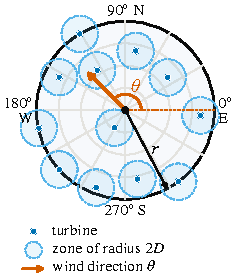
\includegraphics[width=\linewidth]{figures_final/fig_wind_farm.pdf}\\[-2pt]{\small (a)}
\end{minipage}\hfill
\begin{minipage}[b]{0.35\textwidth}\centering
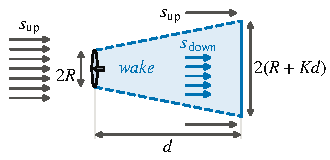
\includegraphics[width=\linewidth]{figures_final/fig_wake_model.pdf}\\[4pt]{\small (b)}
\end{minipage}\hfill
\begin{minipage}[b]{0.35\textwidth}\centering
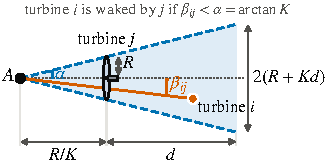
\includegraphics[width=\linewidth]{figures_final/fig_half_cone.pdf}\\[4pt]{\small (c)}
\end{minipage}
\caption{Model geometry. (a) Circular farm of radius $r$ and wind direction $\theta$; the points show, for illustration, a 12-turbine layout ($r=750$~m); discs of radius $2D$ touch at the spacing $\ell_{\min}=4D$. (b) Jensen top-hat wake behind a rotor of radius $R$: width $2(R+Kd)$ at the downstream distance $d$, uniform speed $s_{\text{down}}<s_{\text{up}}$. (c) Wake half cone of turbine $j$ ($K$ exaggerated): virtual vertex $A$ at $R/K$ upstream of the rotor, half-angle $\alpha=\arctan K$; turbine $i$ is waked by $j$ if $\beta_{ij}<\alpha$.}
\label{fig:model}
\label{fig:S-farm}\label{fig:S-wake}\label{fig:S-halfcone}
\end{figure}

\subsection{Wind Model and Direction Discretization}
\label{sec:wind}
For each direction, the wind speed $s$ has the Weibull density $p_s(s;\zeta,\psi)=(\zeta/\psi)\allowbreak(s/\psi)^{\zeta-1}\allowbreak\exp[-(s/\psi)^{\zeta}]$ with shape $\zeta(\theta)$ and scale $\psi(\theta)$. The benchmark rose is piecewise constant: $N_\theta=24$ direction bins $[15(l-1),15l)^\circ$, $l=1,\ldots,24$, with probability $p_l$, shape $\zeta=2$ and scale $\psi_l$ (Table~\ref{S-tab:S-wind}). Data Set~I is nearly unidirectional ($\psi=13$~m/s in all bins; 80\% of the probability in bins 6 and 7, i.e., wind from 165$^\circ$ to 195$^\circ$); Data Set~II is a broad rose with scales from 2.6 to 10~m/s and its highest probability in bin~13. Both are synthetic wind roses of the Kusiak--Song benchmark~\cite{Kusiak2010,Bansal2017}, not measurements at a site; the measured wind climates in this study are the 12-sector Weibull roses of the Horns Rev~1 block (Section~\ref{sec:hornsrev-site}) and of a Lillgrund block (Section~\ref{sec:lillgrund}), both optimized in 5$^\circ$ bins, and IEA37 Case Study~1 uses 16 directions at one speed (Section~\ref{sec:setup-beyond}).
% verified: analysis/wflop_model.py (DS1_W, DS1_PSI, DS2_PSI, DS2_W; k = 2); bins 6+7 of DS I: 0.2+0.6 = 0.8, towards 75-105 deg = from 165-195 deg

\emph{Why the direction discretization matters.} The objective evaluates the wake only at the 24 bin centers $\bar\theta_l=(15l-7.5)^\circ$. A top-hat wake is narrow: by the half-cone geometry (Fig.~\ref{fig:model}c), turbine $j$ wakes a turbine $i$ at the distance $\rho\ge R/K$ only for directions within an interval of width $2[\alpha+\arcsin(R/(\rho\sqrt{1+K^2}))]$ around the direction from $j$ to $i$. With $K=0.075$ and $R=38.5$~m ($\alpha=4.29^\circ$, $R/K=513$~m), this width is below the bin spacing of 15$^\circ$ for $\rho>685$~m and tends to $2\alpha=8.6^\circ$. If no bin center lies in this interval, the wake of the pair does not enter the objective (with bins of 5$^\circ$ or finer, every such interval contains a center). Optimized layouts exploit these gaps (with 1$^\circ$ sub-bins, the mean wake loss of PSO-VNS rises by about 1~pp); Section~\ref{sec:direction} reports which conclusions survive a 1$^\circ$ rose, for re-evaluated and for directly optimized layouts.
% verified (numerically with analysis/wflop_model.jensen_deficits on a 0.001-deg grid): waked width of a pair rho apart = 2(alpha + arcsin(R/(rho sqrt(1+K^2)))) exactly for rho >= R/K (rho = 600: 15.915 deg; 1000: 12.979; 2000: 10.779); width = 15 deg at rho = 685.4 m; alpha = arctan 0.075 = 4.289 deg; R/K = 513.3 m; 2 alpha = 8.58 deg > 5 deg. For rho < R/K the non-physical upstream deficit widens the interval further.
% CHECK-DIR [F03]: loss rise of every method, PSO-VNS 1.322 -> 2.335; [F05]: VNS-based methods and PSO rise most

\subsection{Wake Effect Model}
In the Jensen model (Fig.~\ref{fig:model}b,c), the wake of turbine $j$ is a half cone with half-angle $\alpha=\arctan K$ (wake-spreading constant $K$), and its virtual vertex lies $R/K$ upstream of the rotor. With $u_{ij}=(x_i - x_j)\cos\theta + (y_i - y_j)\sin\theta + R/K$ and the lateral offset $v_{ij}=-(x_i - x_j)\sin\theta + (y_i - y_j)\cos\theta$, turbine $i$ lies in the wake if $\beta_{ij}=\cos^{-1}\!\bigl(u_{ij}/\sqrt{u_{ij}^2+v_{ij}^2}\bigr)<\alpha$. Its downstream distance is $d_{ij}=\lvert u_{ij}-R/K\rvert$, and with the thrust coefficient $C_T$ the velocity deficit is
\begin{equation}
    \Delta_{ij} = 1-\frac{s_{\text{down}}}{s_{\text{up}}}=\frac{1 - \sqrt{1 - C_T}}{\left(1 + K d_{ij}/R\right)^2}.
    \label{eq:deficit}
\end{equation}
The numerator is the deficit behind the rotor from actuator-disc momentum theory, and the factor $R^2/(R+Kd_{ij})^2$ spreads it over the growing wake (Fig.~\ref{fig:model}b); with $C_T=0.8$ and $K=0.075$, a turbine $\ell_{\min}=308$~m directly behind another loses 21.6\% of the wind speed, one 770~m ($10D$) behind 8.8\%.
% verified: (1-sqrt(0.2))/(1+0.075*308/38.5)^2 = 0.2159; (1-sqrt(0.2))/(1+0.075*770/38.5)^2 = 0.0884
As in~\cite{Kusiak2010}, this top-hat wake is tested at the hub center only, so the deficit jumps at the cone edge, and it also reaches a turbine less than $R/K$ \emph{upstream} of $j$ near its axis (between $A$ and the rotor in Fig.~\ref{fig:model}c; non-physical, kept for comparability with the published results). The deficits are combined by the root-sum-square rule,
\begin{equation}\label{eq5}
\Delta_i(\theta) = \Bigl( \textstyle\sum_{j \ne i,\ \beta_{ij} < \alpha} \Delta_{ij}^2 \Bigr)^{1/2} .
\end{equation}
As $C_T$ is constant (which overstates the deficits above rated speed), $\Delta_i(\theta)$ depends only on the layout and the direction, not on the free-stream speed $s$; the local wind speed in a direction bin, $s_{\rm local}=[1-\Delta_i(\theta)]\,s$, is therefore a scaled Weibull variable, with the same shape $\zeta(\theta)$ and the scale $\psi_i(\theta)=\psi(\theta)[1-\Delta_i(\theta)]$. The Horns Rev~1 model (Section~\ref{sec:hornsrev-site}) instead takes $C_T$ from the V80 thrust curve at the free-stream speed of each 1-m/s speed bin and sums the power over these bins, so it does not use this scaling (Section~\ref{S-sec:S-hrmodel}). The hub-center test makes the objective jump where a hub crosses a cone edge in an evaluated direction; hence the derivative-free local search of VNS (Section~\ref{sec:vns}), and finite-difference gradients handicap MS-SLSQP.

\emph{Why the Jensen model.} First, the Jensen model with the benchmark settings is needed for comparability with the published Kusiak--Song results~\cite{Kusiak2010,Bansal2017}, and it is cheap enough for the 52{,}930 optimization runs of this study (Table~\ref{tab:design}). Second, the research question concerns the optimizers and the protocol rather than the fidelity of the wake model; whether the conclusions carry over to another wake model is an empirical question. Third, we therefore test a Gaussian wake in two ways: the methods are re-optimized under the simplified Bastankhah Gaussian wake of IEA37 Case Study~1 (Section~\ref{sec:iea37}), and the final benchmark layouts are re-evaluated with the Gaussian wake of~\cite{Bastankhah2014} (Section~\ref{sec:gaussian}). Control-oriented models, which describe the wake deflection of yawed turbines for wake steering~\cite{Gebraad2016,Bastankhah2016}, add yaw angles as decision variables and turn the problem into a layout--control co-design, which is outside the scope of this study.

\subsection{Power Model and Expected Energy}
\label{sec:powermodel}
\label{sec:S-power}
The power curve of the Kusiak--Song benchmark~\cite{Kusiak2010} is $f(s)=0$ for $s<s_{\text{cut-in}}$, $f(s)=\lambda_1 s+\lambda_0$ for $s_{\text{cut-in}}\le s\le s_{\text{rated}}$ and $f(s)=P_{\text{rated}}$ above, with $s_{\text{cut-in}}=3.5$~m/s, $s_{\text{rated}}=14$~m/s, $P_{\text{rated}}=1500$~kW, $\lambda_1=140.86$ and $\lambda_0=-500$. We use it as published: it is slightly negative just above the cut-in speed ($-7.0$~kW at 3.5~m/s, zero at 3.55~m/s), jumps from 1472 to 1500~kW at the rated speed and has no cut-out speed. We keep this linearized curve for comparability with the published Kusiak--Song results; its effect on the energy values is quantified with a cubic curve in Section~\ref{sec:powercurve}, and the Horns Rev~1 block uses the tabulated V80 power curve (Section~\ref{sec:hornsrev-site}). The expected power of turbine $i$,
\begin{equation}\label{eq8}
E(P_i) = \int_0^{360} p_\theta(\theta) \int_0^{\infty} f(s)\,
       p_s\bigl(s; \zeta(\theta), \psi_i(\theta)\bigr) \, ds \, d\theta ,
\end{equation}
is evaluated, as in~\cite{Kusiak2010}, by a Riemann sum over direction bins $\theta_0 = 0^\circ, \theta_1, \ldots, \theta_{N_\theta} = 360^\circ$ with probabilities $p_l$, and over the speed range between $s_{\text{cut-in}}$ and $s_{\text{rated}}$, divided into $N_s$ bins $s_0 = s_{\text{cut-in}}, s_1, \ldots, s_{N_s} = s_{\text{rated}}$ (benchmark: $N_\theta=24$ bins of 15$^\circ$ and $N_s=21$ bins of 0.5~m/s). With the bin centers $\bar\theta_l=(\theta_{l-1}+\theta_l)/2$ and the Weibull survival function $W_i(s,\theta)=\exp\{-[s/\psi_i(\theta)]^{\zeta(\theta)}\}$ of the local speed,
\begin{equation}
\begin{split}
E(P_i) ={}& \sum_{l=1}^{N_\theta} (\theta_l - \theta_{l-1})\, p_l \Bigg\{ P_{\text{rated}}\, W_i(s_{\text{rated}},\bar\theta_l)
+\lambda_1 \sum_{q=1}^{N_s} \tfrac{s_{q-1} + s_q}{2}\bigl[W_i(s_{q-1},\bar\theta_l)-W_i(s_q,\bar\theta_l)\bigr]\\
&\qquad+ \lambda_0 \bigl[W_i(s_{\text{cut-in}},\bar\theta_l)-W_i(s_{\text{rated}},\bar\theta_l)\bigr] \Bigg\}.
\end{split}
\label{eq:S-power}
\end{equation}
Like the earlier studies, we keep the bin-width factor $(\theta_l-\theta_{l-1})$ in degrees; with 24 bins of $15^\circ$ and $\sum_l p_l=1$, the benchmark objective $\sum_i E(P_i)$ is thus 15 times the expected farm power in kW, and the gross (wake-only) annual energy production is $\mathrm{AEP}\,[\mathrm{MWh}] = (\text{objective}/15)\times 8.76$. The wake-free benchmark objective of one turbine, $E_{\rm ideal}$, is~\eqref{eq:S-power} with $\psi_i=\psi$; for Data Set~I, $E_{\rm ideal}=14{,}045.74$, which corresponds to 936.38~kW (a capacity factor of 62\%, far above real sites) or 8,202.7~MWh/yr.
% verified: 14045.74/15 = 936.38 kW; 936.38/1500 = 0.624; 936.38*8.76 = 8202.7 MWh (reproduced from wflop_model.py); N_s = (14-3.5)/0.5 = 21 (wflop_model.expected_power_linear); 140.86*3.5-500 = -6.99; 500/140.86 = 3.55; 140.86*14-500 = 1472.0

\subsection{Optimization Problem and Constraint Handling}
\label{sec:constraints}
With the wake loss $L(\mathbf X)=N E_{\rm ideal}-\sum_{i=1}^{N}E(P_i)$, reported in percent of the wake-free value, $100\,L/(NE_{\rm ideal})$, the problem is
\begin{equation}
\min_{\mathbf X\in[-r,r]^{2N}} L(\mathbf X)\quad\text{s.t.}\quad \ell_{ij}\ge\ell_{\min}\ (1\le i<j\le N),\qquad x_i^2+y_i^2\le r^2\ (1\le i\le N),
\label{eq:wflop}
\end{equation}
which is equivalent to maximizing the expected farm power and hence the AEP: a problem in $2N$ variables ($2N\le30$ on the benchmark) with a discontinuous objective and $N(N-1)/2$ nonconvex spacing constraints.
After every position update, each coordinate is clipped to $[-r,r]$ (box repair; the square, not the circle). The constraints are handled by a penalty on the violations $g^{\rm b}_{i}=x_i^2+y_i^2-r^2$ and $g^{\rm s}_{ij}=\ell_{\min}-\ell_{ij}$; all optimizers except MS-SLSQP minimize the penalized wake loss
\begin{equation}
\begin{split}
F_p(\mathbf X)={}&\Bigl(N E_{\rm ideal}-\sum_{i=1}^{N}E(P_i)\Bigr)+\sum_{i:\,g^{\rm b}_i>0}\bigl(1+\mu g^{\rm b}_i\bigr)^2\\
&+\sum_{i<j:\,g^{\rm s}_{ij}>0}\bigl(1+\mu g^{\rm s}_{ij}\bigr)^2,\qquad \mu=10^{10},
\end{split}
\label{eq:penalty}
\end{equation}
whose first term is the wake loss $L(\mathbf X)$ reported in our tables. Any violation above about $4.6\times10^{-8}$ (m or m$^2$) makes the penalty exceed any possible wake loss, so comparing $F_p$ values is, up to smaller violations, a feasibility-first rule (feasible before infeasible, then wake loss or total penalty). The scaling ($g^{\rm b}_i$ in m$^2$, $g^{\rm s}_{ij}$ in m) favors infeasible layouts with turbines slightly too close, or with a turbine clipped to the box near a tangent point $(\pm r,y_i)$, where $g^{\rm b}_i=y_i^2$. MS-SLSQP minimizes the wake loss under explicit constraints. A final layout counts as feasible if $\ell_{ij}\ge\ell_{\min}$ and $\sqrt{x_i^2+y_i^2}\le r$ hold within $10^{-6}$~m (Section~\ref{sec:setup}), a looser tolerance than the penalty's. With random starts, no optimizer guarantees a feasible final layout; infeasible final layouts are therefore counted, reported and ranked below feasible ones (Section~\ref{sec:setup-stats}). Section~\ref{sec:boundary} tests an alternative: Deb's feasibility rules~\cite{Deb2000} on dimensionless violations, with box clipping or radial projection.
% verified: largest benchmark wake loss < 15 x 14045.74 = 2.107e5 (plus the small negative part of f); (sqrt(2.2e5)-1)/1e10 = 4.6e-8
% CHECK-DIAG [D06]/[D21]: old-setting infeasible finals (1e-6 m rule) mostly spacing-only; boundary violations = turbine with a coordinate on the box bound (tangent-point pinning); numbers in 06_results sec:psosetting

% end optA/sw/03_model.tex

% begin optA/sw/04_methods.tex
\section{Preliminaries: Phase-1 Methods and Basic VNS}
\label{sec:prelim}
% Proposition environment (neither IEEEtran nor elsarticle defines one); guarded, so a main file may define it in its preamble instead.
\makeatletter\@ifundefined{proposition}{\newtheorem{proposition}{Proposition}}{}\makeatother
A population method keeps $N_p$ candidate vectors $\mathbf X^i\in\mathbb R^{n}$ with components $X^i_m$ and bounds $lb_m=-r$, $ub_m=r$; unless stated otherwise, one iteration costs $N_p$ objective evaluations. This section states the methods exactly as implemented (Algorithms~\ref{alg:pso}--\ref{alg:vns}); Table~\ref{tab:params} collects all settings.

\subsection{PSO and Its Stability Conditions}
\label{sec:pso}
We use the canonical global-best PSO~\cite{Kennedy1995} in the inertia-weight form~\cite{Shi1998} (Algorithm~\ref{alg:pso}). Particle $i$ has a position $\mathbf X^i$, a velocity $\mathbf V^i$ and a personal best $\mathbf P^i$, the swarm keeps the global best $\mathbf G$, and a particle moves by
\begin{align}
\mathbf V^i&\leftarrow w\,\mathbf V^i+c_1\boldsymbol\rho_1\circ\bigl(\mathbf P^i-\mathbf X^i\bigr)+c_2\boldsymbol\rho_2\circ\bigl(\mathbf G-\mathbf X^i\bigr),\label{eq:pso-v}\\
\mathbf X^i&\leftarrow\mathbf X^i+\mathbf V^i,\label{eq:pso-x}
\end{align}
where $\boldsymbol\rho_1,\boldsymbol\rho_2$ are vectors of independent $U(0,1)$ numbers, drawn anew for every move, and $\circ$ is the componentwise product. The constriction PSO of Clerc and Kennedy~\cite{Clerc2002} with their standard choice $\varphi_1=\varphi_2=2.05$ (constriction factor $\kappa=0.7298$) is identical to~\eqref{eq:pso-v} with
\begin{equation}
w=0.7298,\qquad c_1=c_2=\kappa\varphi_1=1.49618 .
\label{eq:constriction}
\end{equation}
PSO denotes~\eqref{eq:pso-v} and~\eqref{eq:pso-x} with these coefficients, fixed a priori from the literature, and the \emph{old setting} the same algorithm with $w=0.7$, $c_1=c_2=2$, i.e., the acceleration coefficients of the original PSO~\cite{Kennedy1995} combined with an inertia weight. Both are run as implemented: velocities start at zero and are not clamped (no $V_{\max}$), a coordinate clipped to the square (Section~\ref{sec:constraints}) keeps its velocity, and $\mathbf P^i$, $\mathbf G$ are updated after each evaluation (asynchronous global best).

\begin{algorithm}[!t]
\caption{PSO as implemented ($N_p(T+1)$ evaluations).}
\label{alg:pso}
\small
\begin{algorithmic}[1]
\State Draw (seeded) and evaluate $N_p$ layouts $\mathbf X^i$; $\mathbf V^i\gets\mathbf 0$, $\mathbf P^i\gets\mathbf X^i$, $\mathbf G\gets\arg\min_i F_p(\mathbf P^i)$
\For{$t=1,\ldots,T$ and $i=1,\ldots,N_p$}
    \State Draw $\boldsymbol\rho_1,\boldsymbol\rho_2\sim U(0,1)^n$; update $\mathbf V^i$ by~\eqref{eq:pso-v} \Comment{no velocity clamping}
    \State $\mathbf X^i\gets\operatorname{clip}(\mathbf X^i+\mathbf V^i,-r,r)$ \Comment{box repair; $\mathbf V^i$ is kept}
    \State Evaluate $F_p(\mathbf X^i)$; replace $\mathbf P^i$ and $\mathbf G$ if it is strictly lower than theirs
\EndFor
\State \Return $\mathbf G$
\end{algorithmic}
\end{algorithm}

\emph{Stability under stagnation.} Consider one coordinate $x=X^i_m$ with $v=V^i_m$, $p=P^i_m$ and $g=G_m$, and assume (A1) \emph{stagnation}, $p$ and $g$ fixed, and (A2) \emph{no active bound}, so that $v_t=x_t-x_{t-1}$. With $\varphi_{k,t}=c_k\rho_{k,t}$ and $\varphi_t=\varphi_{1,t}+\varphi_{2,t}$, every coordinate then follows the random linear recursion $x_{t+1}=(1+w-\varphi_t)\,x_t-w\,x_{t-1}+\varphi_{1,t}\,p+\varphi_{2,t}\,g$, whose random coefficient $\varphi_t$ has mean $\mu=(c_1+c_2)/2$ and variance $\sigma^2=(c_1^2+c_2^2)/12$. The update is \emph{order-1} (\emph{order-2}) \emph{stable} if $\mathrm E\,x_t$ (and $\mathrm E\,x_t^2$) converges to a limit independent of $(x_0,x_1)$~\cite{Poli2009}. Proposition~\ref{prop:pso-stability} applies these known stagnation results~\cite{Poli2009,Bonyadi2017} to the implemented update rule; it is not claimed as new theory.

\begin{proposition}\label{prop:pso-stability}
Let $c_1,c_2\ge0$, $c_1+c_2>0$, and assume (A1)--(A2).
\begin{enumerate}
\item[(a)] $\mathrm E\,x_t\to x^*=(c_1p+c_2g)/(c_1+c_2)$ for all initial values if and only if $\lvert w\rvert<1$ and $0<c_1+c_2<4(1+w)$.
\item[(b)] The update is order-2 stable if and only if $\lvert w\rvert<1$ and
\begin{equation}
\varrho(1):=2\mu(1-w^2)-(1-w)\mu^2-(1+w)\sigma^2>0 .
\label{eq:pso-o2}
\end{equation}
For $c_1=c_2$, \eqref{eq:pso-o2} is Poli's condition~\cite{Poli2009}
\begin{equation}
c_1+c_2<\frac{24\,(1-w^2)}{7-5w};
\label{eq:poli}
\end{equation}
for $c_1\ne c_2$ with the same sum $c_1+c_2$, it is stricter.
\item[(c)] Under (b), $\operatorname{Var}x_t\to V_\infty=(1+w)\,q/\varrho(1)$ with $q=c_1^2c_2^2(p-g)^2/[6(c_1+c_2)^2]$, for $c_1=c_2=c$, $V_\infty=c(1+w)(p-g)^2/(4[12(1-w^2)-c(7-5w)])$; $V_\infty=0$ if and only if $c_1c_2(p-g)=0$. When $c_1,c_2>0$, this is equivalent to $p=g$.
\end{enumerate}
\end{proposition}
\begin{proof}[Proof sketch]
(a) $e_t=\mathrm E\,x_t-x^*$ obeys $e_{t+1}=(1+w-\mu)\,e_t-w\,e_{t-1}$; both roots of $\lambda^2-(1+w-\mu)\lambda+w$ lie strictly inside the unit circle if and only if $\lvert w\rvert<1$ and $\lvert 1+w-\mu\rvert<1+w$ (Schur--Cohn), i.e., $0<\mu<2(1+w)$. (b) With $y_t=x_t-x^*$, $z_t=(\mathrm Ey_t^2,\mathrm Ey_ty_{t-1},\mathrm Ey_{t-1}^2)^{\mathsf T}$ obeys $z_{t+1}=Mz_t+b_t$ with a $3\times3$ matrix $M(w,\mu,\sigma^2)$ and $b_t\to(q,0,0)^{\mathsf T}$, so order-2 stability means a spectral radius of $M$ below one; by Jury's criterion for its characteristic polynomial $\varrho$, this holds iff $\lvert w\rvert<1$ and $\varrho(1)>0$. For $c_1=c_2=c$, $\varrho(1)=c\,[12(1-w^2)-c(7-5w)]/6$; for fixed $c_1+c_2$, $\sigma^2$ is smallest at $c_1=c_2$. (c) $V_\infty$ is the first component of the fixed point of $z\mapsto Mz+(q,0,0)^{\mathsf T}$. Since $(1+w)/\varrho(1)>0$, the variance vanishes exactly when $q=0$, including either zero acceleration coefficient. Full proof: Section~\ref{S-sec:S-th-pso}.
\end{proof}
The order-1 condition involves the \emph{mean} of $\varphi_t$ (with $\varphi=c_1+c_2$, the constant-coefficient condition $\varphi<2(1+w)$ would wrongly call the old setting unstable). For $c_1=c_2$, the region also holds under a weaker, non-stagnant assumption~\cite{Cleghorn2018}. The constriction setting is order-2 stable ($c_1+c_2=2.99<3.35$; spectral radius of $M$ 0.94): in the limit, a coordinate with $P^i_m\ne G_m$ is sampled with mean $(P^i_m+G_m)/2$ and standard deviation $1.04\,\lvert P^i_m-G_m\rvert$, so the swarm keeps sampling around $\mathbf G$ unless $\mathbf P^i=\mathbf G$. The old setting is order-1 stable ($4<6.8$) but beyond the order-2 boundary ($4>3.50$; $c_1=c_2>c^*=1.7486$ at $w=0.7$; spectral radius 1.12), so its second moments grow without bound under stagnation (Fig.~\ref{fig:S-th-stability}; Proposition~\ref{S-prop:S-settings}). Neither condition says how good $\mathbf G$ is, and clipping violates (A2): a clipped coordinate stays at the bound while its kept velocity points outward (Lemma~\ref{S-lem:S-clip}).
\begin{figure}[!t]
\begin{minipage}[c]{0.44\textwidth}\centering
\pipefig{\linewidth}{figures_mpce/theory_stability.pdf}{6cm}
\end{minipage}\hfill
\begin{minipage}[c]{0.53\textwidth}
\caption{Stability regions of the implemented PSO update under stagnation and without active bounds ($c_1=c_2$; Proposition~\ref{prop:pso-stability}). Light: order-1 stable only, $c_1+c_2<4(1+w)$; dark: order-1 and order-2 stable, $c_1+c_2<24(1-w^2)/(7-5w)$. The old setting ($w=0.7$, $c_1=c_2=2$) is order-1 but not order-2 stable; the constriction setting~\eqref{eq:constriction} is order-2 stable.}
\label{fig:S-th-stability}
\end{minipage}
\end{figure}
% CHECK-THEORY [T01]-[T06], [T12]: Proposition prop:pso-stability (full statement of S-prop:S-pso-stability, whose full proof stays in the supplement; order-1 via E[phi]=(c1+c2)/2; Poli's bound exact for c1=c2, analytic region = numerical region, T06); 24(1-0.7^2)/(7-3.5)=3.497; 24(1-0.7298^2)/(7-5*0.7298)=3.348; 4(1+0.7)=6.8; 2*1.49618=2.99; spectral radius of the second-moment matrix 1.124 (old) and 0.944 (constriction) in Table S-th-settings; c* = 3.497/2 = \NSBoundC
% CHECK-THEORY [T05]: SD factor 1.04 = sqrt(V_inf/(p-g)^2) = sqrt(1.0874) (constriction); constant-coefficient misclassification 2(1+0.7) = 3.4 (S-th-pso note); Lemma S-lem:S-clip (b): clipped coordinate stays at the bound while v' >= 0
Section~\ref{sec:psosetting} tests this empirically: in a sweep of $c_1=c_2=c$ at $w=0.7$, feasibility starts to fall near $c^*$ and falls progressively beyond it (to 58.9\% at $c=2$), so the boundary marks approximately where this PSO starts to fail, and velocity clamping largely rescues the old setting. DE's $F=0.5$ exceeds Zaharie's critical value (0.14 at $\mathrm{CR}=0.9$)~\cite{Zaharie2002}, so its weak results are not due to premature variance loss.
% verified (Zaharie): critical F = sqrt((1-CR/2)/N_p) = sqrt((1-0.45)/30)=0.135 (N_p = 30, CR = 0.9, F = 0.5: Section setup); F above the critical value = no variance collapse; Cleghorn2018 cited for c1 = c2 only
% CHECK-CSWEEP [S02]-[S05]: feasibility >= 98 % for c <= 1.7, falls progressively beyond c* = \NSBoundC (\NSFeasCOneEight > \NSFeasCOneNine > \NSFeasCTwoZero at c = 1.8, 1.9, 2.0), onset in the step containing c* ("starts to fall near c*", "marks approximately where ... starts to fail"); [S10]/[S11]: vmax = \NSVmaxFrac (ub-lb) >= 90 % feasible but still worse than constriction ("largely rescues"); details in 06_results
% CHECK-DIAG [D03]/[D06]/[D21]: the diagnostics of the old setting (contraction, spacing-only finals, tangent-point pinning) are stated in 06_results (sec:psosetting), no longer here

\subsection{Salp Swarm Algorithm and Its Laplacian Variant}
\label{sec:ssa}
\label{sec:S-ssa}
The SSA~\cite{Mirjalili2017} (Algorithm~\ref{S-alg:S-ssa}) keeps the best solution found so far as the food source $\mathbf H$ and splits the population, sorted by $F_p$, into leaders and followers. A leader $i\le N_p/2$ updates each coordinate by
\begin{equation}\label{eq:leader}
X_m^i = H_m\pm\xi_1\big((ub_m-lb_m)\xi_2+lb_m\big),
\end{equation}
with either sign with probability $1/2$, $\xi_2\sim U(0,1)$ and $\xi_1=2\exp[-(4t/T)^2]$ decreasing with the iteration $t$ out of $T$: a leader samples $H_m+U(-\xi_1r,\xi_1r)$ in every coordinate, with $\xi_1\le0.037$ for $t\ge T/2$. A follower $i>N_p/2$ moves to the midpoint of its position and the \emph{new} position of the preceding salp. The leaders thus perturb $\mathbf H$ uniformly with a shrinking radius, and the followers only average~\cite{Castelli2022}. This implementation departs from the description of Mirjalili et~al.~\cite{Mirjalili2017} in three points, shared by SSA and LX-SSA: (a) the paper defines a single leader, the first salp, and followers $i\ge2$, whereas the implementation, like the authors' reference MATLAB code, treats the first $N_p/2$ salps as leaders; (b) the paper takes the $+$ sign in~\eqref{eq:leader} if $\xi_3\ge0$ for $\xi_3\sim U(0,1)$, which always holds, whereas the implementation, like the reference code, compares $\xi_3$ with $0.5$ and so takes either sign with probability $1/2$; (c) the salps are re-sorted by $F_p$ after every iteration (Algorithm~\ref{S-alg:S-ssa}, line~12), so the leaders are the better half of the current population, whereas the paper only selects the best salp as the food source. SSA and LX-SSA thus follow the reference code in (a) and (b) and the code of the published LX-SSA~\cite{Solanki2023} in all three points, so that both are tested as published. LX-SSA~\cite{Solanki2023} gives each follower a second candidate $Y_m^i=X_m^i+\gamma(H_m-X_m^i)$ with one Laplace step~\cite{Deep2007} for all coordinates,
\begin{equation}
\gamma=\phi-\chi\,\mathrm{sgn}\bigl(z-\tfrac12\bigr)\ln\bigl(1-2\lvert z-\tfrac12\rvert\bigr),\quad z\sim U(0,1),
\label{eq:laplace}
\end{equation}
with $\phi=0$ and $\chi=1$, and keeps the better candidate. As published, it evaluates both candidates of each follower and then re-evaluates the kept ones with the new population, so an iteration costs $2N_p$ evaluations (SSA: $N_p$) and LX-SSA runs half as many iterations as SSA (Table~\ref{tab:params}). Comparing the two tests LX-SSA as published, not the Laplace step alone (for the step itself, see the ablation in Section~\ref{sec:abl-swarm}); both use the code of the published LX-SSA study~\cite{Solanki2023}.

\emph{Laplace step.} Eq.~\eqref{eq:laplace} draws $\gamma$ by inverse-CDF sampling from a Laplace distribution with location $\phi$ and scale $\chi$: the sign of $\gamma-\phi$ is that of $z-\tfrac12$, and $\lvert\gamma-\phi\rvert=-\chi\ln(1-2\lvert z-\tfrac12\rvert)$ is exponential with mean $\chi$. With $\phi=0$, the step is centered on $\mathbf X^i$: a move toward $\mathbf H$ ($\gamma>0$) and one away from it ($\gamma<0$) are equally likely, and, as $\gamma$ is a scalar, $\mathbf Y^i$ lies on the line through $\mathbf X^i$ and $\mathbf H$ (before box repair). With $\chi=1$, $\mathrm E\lvert\gamma\rvert=1$, i.e., the mean step equals the distance from $\mathbf X^i$ to $\mathbf H$, and $P(\lvert\gamma\rvert>1)=e^{-1}\approx0.37$, so about 18\% of the candidates overshoot $\mathbf H$ ($\gamma>1$); the exponential tails, heavier than Gaussian ones, give occasional long jumps that can aid exploration. The location $\phi=0$ is that of the Laplace crossover of Deep and Thakur~\cite{Deep2007}, who fix it at zero, and $\chi=1$ is the value of the published LX-SSA~\cite{Solanki2023}; we keep both untuned. An ablation designed after the main comparison separates the Laplace step from its cost and varies the distribution of $\gamma$ and the scale $\chi$ (Section~\ref{sec:abl-swarm}): on twelve cases, the step gives no advantage over the SSA midpoint, and $\chi<1$ is worse.
% CHECK-THEORY [T11]: SSA xi_1(T/2) = 2 exp(-4) = 0.0366 ("xi_1 <= 0.037 for t >= T/2"); leader step xi_1((ub-lb) xi_2 + lb) = xi_1 r (2 xi_2 - 1) (S-th-feas note)
% verified: analysis/authors_optimizers.py SSA/LXSSA: leaders = pop_size // 2 = 15; follower = (pop[i] + new_pop[i-1])/2; LX: one scalar gamma per follower, candidate = pop[i] + gamma (food - pop[i]); both clipped and evaluated, then whole population evaluated (2 N_p per iteration)

% Page budget: the SSA/LX-SSA pseudocode stays in the supplementary material (Algorithm S-alg:S-ssa); main-text version was:
% \begin{algorithm}[!t]
% \caption{SSA and LX-SSA (LX: LX-SSA only; evaluations in brackets)}
% \label{alg:S-ssa}
% \small
% \begin{algorithmic}[1]
% \State Draw and evaluate $N_p$ salps; sort them by $F_p$ and set the best as food source $\mathbf H$. \Comment{[$N_p$]}
% \For{$t=1$ to $T$}
%     \State Update $\xi_1=2\exp[-(4t/T)^2]$.
%     \State Leaders $i\le N_p/2$: new position $\tilde{\mathbf X}^i$ by \eqref{eq:leader}.
%     \For{followers $i=N_p/2+1,\ldots,N_p$}
%         \State $\tilde{\mathbf X}^i\gets\mathbf Z^i=\tfrac{1}{2}(\mathbf X^i+\tilde{\mathbf X}^{i-1})$
%         \State LX: form $\mathbf Y^i$ by \eqref{eq:laplace}, box-repair $\mathbf Y^i$ and $\mathbf Z^i$, evaluate both, $\tilde{\mathbf X}^i\gets$ the better \Comment{[2 per follower]}
%     \EndFor
%     \State Box-repair $\tilde{\mathbf X}$, set $\mathbf X\gets\tilde{\mathbf X}$, evaluate $F_p$ for all salps, sort them, and update $\mathbf H$. \Comment{[$N_p$]}
% \EndFor
% \State \Return $\mathbf H$.
% \end{algorithmic}
% \end{algorithm}

\subsection{Basic Variable Neighborhood Search}
\label{sec:vns}
The basic VNS~\cite{Mladenovic1997,Hansen2001}, in the continuous form of~\cite{Mladenovic2008} (Algorithm~\ref{alg:vns}), improves one incumbent $\mathbf X$ with $k_{\max}=5$ $\ell_\infty$ shell neighborhoods $\mathcal N_k(\mathbf X)=\{\mathbf X':\delta_{k-1}<\lVert \mathbf X'-\mathbf X\rVert_\infty\le\delta_k\}$, $\delta_k=0.1\,k\,r$, of the whole layout: shaking draws a uniform point of $\mathcal N_k(\mathbf X)$, clipped to the box, and a best-improvement local search improves it. As the top-hat wake makes $F_p$ discontinuous, the local search is a compass search: it evaluates all $2n$ moves $\pm h\,\mathbf e_m$ ($\mathbf e_m$ the $m$th unit vector; 60 evaluations for $N=15$), moves to the best one if it strictly improves, and halves $h$ (from $h_0=0.05r$) when none does, until $h<h_{\min}=10^{-3}r$. A completed descent ends at a point that no move $\pm\bar h\,\mathbf e_m$, $\bar h=h_0/2^5=0.0015625\,r$, improves (Proposition~\ref{S-prop:S-ls}), a coordinate-wise optimality at one step length, not a local minimum.
% CHECK-THEORY [T12]: compass search final step h0/2^5 = 0.0015625 r (Proposition S-prop:S-ls); verified: analysis/original_vns.py (k_max = 5, rho_k = 0.1 k r, h0 = 0.05 r, h_min = 1e-3 r; move to the best of the 2 dim moves if it improves the current point, else halve h; shaking by rejection in the l_inf shell, then clip)

\begin{algorithm}[!t]
\caption{Basic VNS from an incumbent $\mathbf X$ (until the budget is used; returns the best layout evaluated).}
\label{alg:vns}
\small
\begin{algorithmic}[1]
\State $\mathbf X\gets\textsc{LocalSearch}(\mathbf X)$; $k\gets1$
\Loop
    \State Draw $\mathbf d\sim U[-\delta_k,\delta_k]^n$ until $\lVert\mathbf d\rVert_\infty>\delta_{k-1}$; evaluate $\mathbf X'=\operatorname{clip}(\mathbf X+\mathbf d)$ \Comment{shaking}
    \State $\mathbf X'\gets\textsc{LocalSearch}(\mathbf X')$; \textbf{if} $F_p(\mathbf X')<F_p(\mathbf X)$ \textbf{then} $\mathbf X\gets\mathbf X'$, $k\gets1$ \textbf{else} $k\gets k\bmod k_{\max}+1$
\EndLoop
\Function{LocalSearch}{$\mathbf y$} \Comment{compass search, best improvement}
    \State $h\gets h_0$; \textbf{while} $h\ge h_{\min}$: evaluate the $2n$ points $\operatorname{clip}(\mathbf y\pm h\,\mathbf e_m)$; if the best, $\mathbf y'$, has $F_p(\mathbf y')<F_p(\mathbf y)$, then $\mathbf y\gets\mathbf y'$, else $h\gets h/2$
    \State \Return $\mathbf y$
\EndFunction
\end{algorithmic}
\end{algorithm}

\section{Two-Phase Swarm--VNS Design and PSO-VNS}
\label{sec:hybrid}

\subsection{Two-Phase Template}
\label{sec:template}
All hybrids follow one sequential (relay) template. For a budget of $B$ evaluations and a split $\omega\in(0,1)$, Phase~1 starts from the seeded initial population, runs a population method for about $\omega B$ evaluations and passes its best layout to Phase~2, the basic VNS (Algorithm~\ref{alg:vns}), which applies the local search to it and then iterates until $B$ evaluations are used. Only Phase~1 differs: PSO in \emph{PSO-VNS}; SSA or LX-SSA in \emph{SSA-VNS} and \emph{LX-SSA-VNS} (with $\xi_1$ compressed to the Phase-1 iterations); and, in the controls, $\operatorname{round}(\omega B)$ layouts: the initial population, then layouts drawn uniformly in the farm disc (\emph{RSD-VNS}) or in its bounding square (\emph{RS-VNS}). VNS alone is the limiting case in which Phase~1 is the initial population. Phase~1 runs for $T_1=\operatorname{round}((\omega B-N_p)/c)$ iterations of $c$ evaluations ($c=N_p$ for PSO and SSA, $2N_p$ for LX-SSA). A swarm phase is useful only if it gives VNS a better start than random sampling with about the same number of evaluations (at $\omega=0.5$, 3,015 for the controls and 3{,}030 for the swarms ($N_p(T_1+1)$; LX-SSA: $N_p(2T_1+1)$)); the component analysis (Section~\ref{sec:ablation}) tests this for each Phase-1 choice against RSD-VNS, with RS-VNS as a weak minimum bar, as the following elementary result, an application of basic geometric probability to the implemented sampling, shows.

\begin{proposition}\label{prop:S-box}
Let the $2N$ coordinates be independent and uniform in $[-r,r]$, and let $P_N$ be the probability that the layout is feasible (all turbines in the disc $\mathcal D$ of radius $r$ and all pairwise distances $\ge s$). Then (a) all $N$ turbines lie in $\mathcal D$ with probability $(\pi/4)^N$; (b) $P_N\le(\pi/4)^N\prod_{k=1}^{N-1}\max\bigl\{0,\ 1-\max\{A(s),\,k\,A(s/2)\}/(\pi r^2)\bigr\}$, where $A(\rho)$ is the area of the part of $\mathcal D$ covered by a disc of radius $\rho$ centered on the boundary of $\mathcal D$ (closed form: \eqref{S-eq:S-th-lens}); (c) among $M$ such layouts, the expected number of feasible ones is $MP_N$.
\end{proposition}
\begin{proof}
(a) The turbines are independent and uniform in the square, each in $\mathcal D$ with probability $\pi r^2/(2r)^2$. (b) Given (a), the positions $\mathbf p_1,\ldots,\mathbf p_N$ are independent and uniform in $\mathcal D$. If $\mathbf p_1,\ldots,\mathbf p_k$ are pairwise at least $s$ apart, $\mathbf p_{k+1}$ must avoid $U_k=\mathcal D\cap\bigcup_{j\le k}B(\mathbf p_j,s)$. The area of $B(\mathbf c,\rho)\cap \mathcal D$, $\mathbf c\in \mathcal D$, is nonincreasing in $\lVert\mathbf c\rVert$ (its derivative is minus the length of the common chord), hence $\ge A(\rho)$; so $\lvert U_k\rvert\ge A(s)$, and, as the discs $B(\mathbf p_j,s/2)\subset B(\mathbf p_j,s)$ are disjoint, $\lvert U_k\rvert\ge kA(s/2)$. The chain rule over $k$ gives (b). (c) Linearity of expectation.
\end{proof}
The bound (b) is loose; by Monte Carlo, $P_N<10^{-6}$ for the largest cases ($N=12$, 15; $N=10$: no feasible layout in $10^7$), so the 3,015 samples of RS-VNS contain about $10^{-3}$ or fewer feasible layouts in expectation (Table~\ref{S-tab:S-th-box}), and RS-VNS hands VNS the least-violating sample. The spacing dominates ($P_N\ll(\pi/4)^N$): 730 RS-VNS runs have no feasible sample, and disc sampling gives one in only 242 of them.
% CHECK-THEORY [T07]-[T10]: Proposition prop:S-box (= S-prop:S-box, restored in the main text with its proof; R1-6 had moved it to the supplement): (pi/4)^N, rigorous spacing bound (lens area nonincreasing, T10), Monte Carlo P_N < 1e-6 for N = 12, 15 (N = 10: 0 of 1e7), expected feasible of 3,015 <= 1.0e-3 (Table S-tab:S-th-box)
% CHECK-DIAG [D17]: RS-VNS Phase-1 replay agrees with the runs and with (pi/4)^N; \NDRsRunsNoFeasSample (= \NRSRunsNoFeasSample) runs without any feasible Phase-1 sample
% CHECK-FINAL [C60]: spacing binding (R3-6): of the \NRSRunsNoFeasSample RS-VNS runs without a feasible sample, disc sampling (RSD-VNS, same runs) rescues \NRsSquareExplains < \NRsSpacingDominates that stay without one ("mainly because of the spacing"); [C61]: controls switch at 3,015, swarms at 3,030; RSD-VNS definition: mpce_experiments.RSDVNS (first 30 = common initial population, then polar-uniform disc samples)

\subsection{PSO-VNS}
PSO-VNS (Algorithm~\ref{alg:hybrid}) is not a new PSO variant: its Phase~1 is the plain PSO of Algorithm~\ref{alg:pso} and, as the coefficients do not depend on the iteration, reproduces exactly, for a given seed, the first $N_p(T_1+1)$ evaluations of a PSO run (Proposition~\ref{S-prop:S-prefix}); comparing PSO-VNS with PSO thus isolates the effect of Phase~2. This does not hold for SSA-VNS and LX-SSA-VNS, whose $\xi_1$ depends on $t/T_1$.

\begin{algorithm}[!t]
\caption{PSO-VNS for a prescribed turbine count $N$.}
\label{alg:hybrid}
\small
\begin{algorithmic}[1]
\Require budget $B$, split $\omega$, $N_p$, $w$, $c_1$, $c_2$, radius $r$, $k_{\max}$
\State $\mathbf G\gets$ PSO (Algorithm~\ref{alg:pso}) with $T=T_1=\operatorname{round}((\omega B-N_p)/N_p)$ \Comment{Phase 1}
\State $\mathbf X\gets\textsc{LocalSearch}(\mathbf G)$; $k\gets1$ \Comment{Phase 2 (Algorithm~\ref{alg:vns})}
\While{fewer than $B$ evaluations have been used}
    \State $\mathbf X'\gets\textsc{LocalSearch}(\text{uniform point of }\mathcal N_k(\mathbf X))$; \textbf{if} $F_p(\mathbf X')<F_p(\mathbf X)$ \textbf{then} $\mathbf X\gets \mathbf X'$, $k\gets1$ \textbf{else} $k\gets k\bmod k_{\max}+1$
\EndWhile
\State \Return best layout evaluated
\end{algorithmic}
\end{algorithm}


PSO-VNS adds one parameter to PSO and VNS, the split $\omega$; with $\omega=0.5$ and $B=6{,}030$, PSO runs for $T_1=100$ iterations (99.5 rounded half to even) and VNS receives 3,000 evaluations (Table~\ref{tab:params}). None of these values was tuned; Section~\ref{sec:split} studies $\omega$. At this budget, PSO-VNS is essentially PSO plus one compass-search descent, and the neighborhoods matter only for small $N$ (Section~\ref{sec:abl-vns}).
% CHECK-DIAG [D08]: essentially one compass-search descent (median shaking steps \NDShakesPSOVNS, first descent \NDDescentSharePSOVNS % of the Phase-2 improvement; 12 split cases x 10 seeds; same pattern for SSA-VNS, RS-VNS); [D20]: cycles \NDCycleEvalsPctPSOVNS % of the Phase-2 evaluations pooled (median run \NDCycleEvalsPctMedianPSOVNS %), accepted cycles \NDCycleSharePSOVNS % of the gain (\NDCycleAllSharePSOVNS % incl. the cycle cut off by the budget)
% CHECK-DIAG [D09]: N >= 12: first descent unfinished in \NDDescentUnfinishedLargePSOVNS of \NDRunsLargePSOVNS runs, median run without shaking ("neighborhoods matter only for small N")
% verified: Python round(99.5) = 100 (half to even); omega = 0.25/0.75/0.9 give 49/150/180

Table~\ref{tab:params} lists the settings of all methods, the published defaults~\cite{Clerc2002,Mirjalili2017,Solanki2023,Storn1997,Mladenovic2008}; MS-SLSQP (SciPy's SLSQP~\cite{Kraft1988}) minimizes $L$ under the scaled constraints of~\eqref{eq:wflop} (Section~\ref{S-sec:S-slsqp}). At 30,030 and 120,030 evaluations (Section~\ref{sec:budget}), $T$ and $T_1$ follow the same rules.
\begin{table}[!t]
\centering
\caption{Settings of all methods at the benchmark budget $B=6{,}030$ evaluations (including the initial population and, for MS-SLSQP, the finite-difference calls); $N_p=30$; box repair by clipping to $[-r,r]$. A population method uses $N_p(T+1)$ evaluations, LX-SSA $N_p(2T+1)$.}
\label{tab:params}
\scriptsize\setlength{\tabcolsep}{3.5pt}
\begin{tabular}{@{}>{\raggedright\arraybackslash}p{0.14\textwidth}>{\raggedright\arraybackslash}p{0.14\textwidth}>{\raggedright\arraybackslash}p{0.68\textwidth}@{}}
\toprule
Method & Iterations & Coefficients and operators \\
\midrule
PSO & $T=200$ & Algorithm~\ref{alg:pso}; $w=0.7298$, $c_1=c_2=1.49618$ (old setting: $w=0.7$, $c_1=c_2=2$); $\mathbf V^i_0=\mathbf 0$, no $V_{\max}$; clipped coordinate keeps its velocity; asynchronous $\mathbf P^i$, $\mathbf G$ \\
SSA & $T=200$ & Algorithm~\ref{S-alg:S-ssa}; 15 leaders, 15 followers; $\xi_1=2\exp[-(4t/T)^2]$ \\
LX-SSA & $T=100$ & as SSA, plus a Laplace candidate per follower, $\phi=0$, $\chi=1$~\eqref{eq:laplace}; both candidates evaluated \\
DE/rand/1/bin & $T=200$ & $F=0.5$, $\mathrm{CR}=0.9$; mutant clipped before crossover; asynchronous one-to-one replacement \\
VNS & 30 initial, then 6,000 & Algorithm~\ref{alg:vns} from the best initial layout; $k_{\max}=5$, $\delta_k=0.1kr$, $h_0=0.05r$, $h_{\min}=10^{-3}r$ \\
MS-SLSQP & $\le200$ per start & SLSQP, $\mathrm{ftol}=10^{-9}$, forward differences (step 1~m); starts: initial layouts by increasing $F_p$, then random layouts \\
PSO-VNS, SSA-VNS, LX-SSA-VNS & $T_1=100$ / 100 / 50 (3,030), then 3,000 & $\omega=0.5$; Phase~1 PSO / SSA / LX-SSA as above ($\xi_1$ over $T_1$), Phase~2 VNS (Algorithm~\ref{alg:vns}) \\
RS-VNS, RSD-VNS & 3,015 samples, then 3,015 & $\omega=0.5$; initial population, then uniform layouts in the square / disc; Phase~2 VNS \\
\bottomrule
\end{tabular}
\end{table}
% verified: analysis/authors_optimizers.py (PSO, DE, SSA, LXSSA), analysis/original_vns.py (BVNS defaults), analysis/hybrid_lxssa_bvns.py (T1 = round((split B - Np)/per_iter)), supplement sec:S-iter and sec:S-slsqp (MS-SLSQP: maxiter 200 per start, ftol 1e-9, eps 1 m, scaled constraints, feasibility threshold -1e-9)

% end optA/sw/04_methods.tex

% begin optA/sw/05_setup.tex
\section{Evaluation Protocol}
\label{sec:setup}

\subsection{Cases and Methods}
\label{sec:setup-cases}
The 68 cases combine the two Kusiak--Song wind data sets~\cite{Kusiak2010,Bansal2017} (Table~\ref{S-tab:S-wind}) with circular farms of radii $r=500$, 750 and 1000~m and $N=2,\ldots,10$, $2,\ldots,12$ and $2,\ldots,15$ turbines ($R=38.5$~m, $\ell_{\min}=4D=308$~m, $C_T=0.8$, $K=0.075$).

The \emph{main comparison} includes eight methods ($N_p=30$ where applicable): PSO-VNS (Algorithm~\ref{alg:hybrid}, $\omega=0.5$); PSO; SSA-VNS; SSA; LX-SSA; DE/rand/1/bin~\cite{Storn1997} (scale factor 0.5, crossover rate 0.9); VNS; and MS-SLSQP, a multistart sequential least-squares programming method (SciPy's SLSQP~\cite{Kraft1988}, forward-difference gradients) that minimizes the wake loss under explicit constraints, restarting from the initial, then random layouts (Section~\ref{S-sec:S-protocol}); all others minimize $F_p$~\eqref{eq:penalty} over $[-r,r]^{2N}$. The \emph{component analysis} (Section~\ref{sec:ablation}) adds LX-SSA-VNS and two random-sampling controls (Section~\ref{sec:template}; for RSD-VNS in other studies see Table~\ref{tab:design}): after the common initial population, \emph{RSD-VNS} samples its Phase-1 layouts uniformly in the farm disc and \emph{RS-VNS} in the bounding square (3,015 layouts versus the hybrids' 3,030 Phase-1 evaluations). A split study varies $\omega$ on twelve cases (Section~\ref{sec:split}). Table~\ref{tab:design} lists all studies; the re-evaluations and diagnostics use stored layouts and runs.

\emph{Choice of the pool.} The pool contains what the research questions need: the PSO baseline in two settings, the salp-swarm methods and their hybrids, the local search alone (VNS), a gradient-based method and the random-sampling controls. In the main comparison, DE/rand/1/bin represents the real-coded evolutionary family, whose operators act directly on the continuous coordinates. In the additional experiments, designed after the main comparison, a standard real-coded GA was run on the 68 cases, and on the Horns Rev~1 block and IEA37 Case Study~1 at 6,030 and 30,030 evaluations ($N_p=30$; binary tournament, SBX~\cite{Deb1995} with $\eta_c=15$ and $p_c=0.9$, polynomial mutation~\cite{DebGoyal1996} with $\eta_m=20$ and $p_m=1/n$ for $n=2N$ variables, clipping to the box and elitism, all untuned); it enters the nine-method benchmark pool of Table~\ref{tab:ga-main} and the site pools of Tables~\ref{tab:hr-site}--\ref{tab:iea-means} (details: Section~\ref{S-sec:S-xp-ga}), not the eight-method analysis. The GAs of~\cite{Mosetti1994,Grady2005} optimize the occupation of grid cells, a discrete formulation that cannot be compared directly on continuous coordinates. ACO~\cite{Eroglu2012}, BBO~\cite{Bansal2017} and adaptive GAs were not re-implemented, to bound the number of runs (Table~\ref{tab:design}); their published results use other budgets and constraint handling (Section~\ref{sec:literature}). The pool is thus a controlled set of baselines and controls, not a survey of WFLOP optimizers (Section~\ref{sec:limits}).
% CHECK-FINAL [C61]: RS-VNS and RSD-VNS switch after round(0.5 x 6,030) = 3,015 Phase-1 evaluations; RSD-VNS = experiment rsdisc (68 cases x 30 seeds only; not in the budget, feasible-start, Horns Rev or IEA37 studies); CHECK-DIAG [D17]: RS-VNS Phase-1 replay

\begin{table}[!htbp]
\centering
\caption{Experimental design. Budget: objective evaluations per run, all counted (initial population, finite-difference evaluations of MS-SLSQP); r: random, f: feasibility-preserving initialization. Runs: optimization runs made for that study (``reused'': taken from another study in this table). Ten methods: the eight of the main comparison, LX-SSA-VNS and RS-VNS. Split cases: middle and largest $N$ per farm and data set; six largest: largest $N$ per farm and data set. In total, 52{,}930 optimization runs (16{,}740 in the additional experiments and sensitivity studies).}
\label{tab:design}
\scriptsize
\setlength{\tabcolsep}{3pt}
\begin{tabular}{@{}>{\raggedright\arraybackslash}p{2.0cm}>{\raggedright\arraybackslash}p{1.85cm}>{\raggedright\arraybackslash}p{5.6cm}>{\raggedright\arraybackslash}p{2.15cm}>{\raggedright\arraybackslash}p{1.05cm}>{\raggedright\arraybackslash}p{1.15cm}>{\raggedright\arraybackslash}p{0.75cm}@{}}
\toprule
Study & Cases & Methods & Budget (init.) & Seeds & Runs & Sec. \\
\midrule
Main comparison & 68 benchmark & PSO-VNS, PSO, SSA-VNS, SSA, LX-SSA, DE, VNS, MS-SLSQP & 6,030 (r) & 1--30 & 16{,}320 & \ref{sec:overall} \\
Component analysis & 68 & LX-SSA-VNS, RS-VNS, RSD-VNS (2{,}040 each); six reused & 6,030 (r) & 1--30 & 6{,}120 & \ref{sec:ablation} \\
Old PSO setting & 68 & PSO, $w=0.7$, $c_1=c_2=2$ & 6,030 (r) & 1--30 & 2{,}040 & \ref{sec:psosetting} \\
Budget split & 12 split cases & PSO-VNS, $\omega=0.25$, 0.75, 0.9 (360 each); $\omega=0.5$, 1 reused & 6,030 (r) & 1--30 & 1{,}080 & \ref{sec:split} \\
Coefficient sweep & 12 split cases & PSO, $w=0.7$, $c_1=c_2=c=1.2$, 1.4, 1.6--2.0 (step 0.1); $c=2$ with $v\gets0$ or $\lvert v\rvert\le0.2\,(u-l)$ (360 each) & 6,030 (r) & 1--30 & 3{,}240 & \ref{sec:psosetting} \\
Budget scaling & six largest & ten methods (6,030 reused) & 30,030; 120,030 (r) & 1--30 & 3{,}600 & \ref{sec:budget} \\
Feasible starts & six largest & ten methods except RS-VNS & 6,030 (f) & 1--30 & 1{,}620 & \ref{sec:feasinit} \\
Horns Rev~1 & 16 turbines & ten methods (f: except RS-VNS) & 6,030 (r, f); 30,030, 120,030 (r) & 1--30; 1--10 at 120,030 & 970 & \ref{sec:hornsrev-site} \\
IEA37 CS~1 & 16, 36 turbines & ten methods & 6,030; 30,030 (r) & 1--30 & 1{,}200 & \ref{sec:iea37} \\
\multicolumn{7}{@{}l}{\emph{Additional experiments and sensitivity studies}} \\
Spacing $5D$, $6D$ & 12 split cases & the eight of the main comparison and RSD-VNS ($4D$: stored runs reused) & 6,030 (r) & 1--30 & 6{,}480 & \ref{sec:spacing} \\
Laplace ablation & 12 split cases & LX-SSA without re-evaluation; Laplace candidate replacing the midpoint; $\gamma\sim U(-2,2)$; $\chi=0.25$, 0.5, 2 (360 each); SSA, LX-SSA reused & 6,030 (r) & 1--30 & 2{,}160 & \ref{S-sec:S-xp-lap} \\
Real-coded GA & 68; Horns Rev~1; IEA37 CS~1 & GA (other methods reused) & 6,030 (r); sites also 30,030 (r) & 1--30 & 2{,}220 & \ref{S-sec:S-xp-ga} \\
Exact gradients & IEA37 CS~1, 16 and 36 turbines & MS-SLSQP and PSO-SLSQP with exact gradients & 6,030; 30,030 (r) & 1--30 & 240 & \ref{S-sec:S-xp-grad} \\
Lillgrund & 16 turbines (block) & the eight of the main comparison and RSD-VNS & 6,030; 30,030 (r) & 1--30 & 540 & \ref{sec:lillgrund} \\
Constraint handling & 6 (3 per data set) & PSO-VNS, PSO, GA, SSA-VNS, DE; three constraint handlings (900 each) & 6,030 (r) & 31--60 & 2{,}700 & \ref{sec:boundary} \\
Direct 1$^\circ$ optimization & 8 (4 per data set) & PSO-VNS, PSO, GA, MS-SLSQP, RSD-VNS; 1$^\circ$ objective and seed-paired 15$^\circ$ control (1{,}200 each) & 6,030 (r) & 31--60 & 2{,}400 & \ref{sec:direction} \\
\midrule
Re-evaluation & stored final layouts & cubic power curve, Gaussian wake (main comparison); 5$^\circ$ and 1$^\circ$ bins: 21{,}716 layouts (11 methods), 1{,}030 Horns Rev~1 and 540 Lillgrund runs (also PyWake NOJ) & -- & -- & -- & \ref{sec:robustness} \\
Diagnostics & 6; 12; 7 & instrumented: PSO (both settings); Phase~2 of PSO-VNS, SSA-VNS, RS-VNS; PSO, DE from feasible starts & as stored & 10; 10; 3 & 522 (reruns) & \ref{S-sec:S-diag} \\
\bottomrule
\end{tabular}
\end{table}
% CHECK (manual, 2026-09-29; run counts derived from the design constants and confirmed by the row counts of the run files in analysis/, no macro unless named):
%   main 8 x 68 x 30 = 16,320 = \NRunsMain; component analysis 3 x 68 x 30 = 6,120 new (LXBV in fresh_bgrid, mpce_rsvns, mpce_rsdisc = \NDRsDiscRuns), \NRunsBenchmark = 16,320 + 6,120 = 11 x 2,040;
%   split: mpce_psosplit 720 rows (omega 0.25 / 0.75) + mpce_omega90 360 rows (\NDOmegaNinetyRuns) = 1,080; csweep: mpce_csweep_s0of1.csv 3,240 rows = 9 settings x \NSRuns;
%   budget: mpce_b30k + b30kp 2,100 rows and mpce_b120k + b120kp 1,900 rows, minus the superseded Horns Rev rows (300 and 100; replaced by hrfix) = 1,800 + 1,800 = 3,600 (10 x 6 x 30 x 2);
%   feasible init.: mpce_feas 1,680 + mpce_feasp 210 = 1,890 rows minus 270 superseded Horns Rev rows = 1,620 (9 x 6 x 30);
%   Horns Rev: mpce_hrfix 970 rows = 10 x 30 (6,030) + 10 x 30 (30,030) + 10 x 10 (120,030) + 9 x 30 (feasible) = \NFHRNRuns;
%   IEA37: mpce_iea16/iea36(+p) 1,200 rows = 10 methods x 2 scenarios x 2 budgets x 30 (Table S-tab:iea37-detail lists all ten; the main-text Table tab:iea37 shows eight);
%   total 22,440 + 2,040 + 1,080 + 3,240 + 3,600 + 1,620 + 970 + 1,200 = 36,190;
%   additional experiments (rev2_*_s*of*.csv): 6,480 + 2,160 + 2,220 + 240 + 540 = 11,640 (47,830 with the above; caption total verified 2026-10-04);
%   sensitivity studies (2026-10-04): rev3_constraint_pen/deb/proj.csv 3 x 900 rows = 2,700 (5 methods x 6 cases x 30 seeds per variant); rev3_fine_s0..9of10.csv 1,200 rows
%   + rev3_fine15_s0of1.csv 1,200 (8 cases x 5 methods x 30 seeds per arm; control arm complete, 1,200 rows) = 2,400;
%   grand total 36,190 + 11,640 + 2,700 + 2,400 = 52,930 (16,740 in the additional experiments and sensitivity studies, designed after the main comparison); re-evaluation: rev3_sites.json hr_eval.n_layouts 1,030 (970 + 60 GA), lg_eval.n_layouts 540;
%   diagnostics \NDVerRuns = 2 x \NDDynRuns + 3 x \NDVnsRunsPSOVNS + \NDFsRunsPSO + \NDFsRunsDE (120 + 360 + 42); CHECK-DIAG [D01], [D17]

\subsection{Comparison Design and Statistics}
\label{sec:setup-stats}
\emph{Equal budgets and paired seeds.} Unless stated otherwise, a run uses exactly $B=6{,}030$ objective evaluations. The budget is a model-query budget: it counts objective calls, including the initial population, finite-difference calls and repeated evaluations of a layout, and charges an exact gradient (IEA37 only) as $c_g=3$ objective equivalents (Section~\ref{sec:iea37}). Optimizer overhead, constraint evaluations, SLSQP subproblems and the geometric packing of the feasibility-preserving initialization are not charged, so equal budgets do not imply equal elapsed times (Section~\ref{sec:runtime}). Each method uses seeds 1--30 and draws its initial population first, so runs with equal seeds share it and are paired.
% verified 2026-09-28: first Curve value identical across fresh_grid/vgrid/bgrid and mpce_psoc/psobv/rsvns/slsqp (13 files) for all 792 case-seed pairs with a feasible initial best (else NaN)

\emph{Feasibility-aware ranking.} Let $f_{a,c}$ be the number of feasible runs of method $a$ in case $c$ (tolerance $10^{-6}$~m; Section~\ref{S-sec:S-tol}) and $\bar L_{a,c}$ the mean wake loss of these runs. Method $a$ is \emph{qualified} in case $c$ if at least half of its runs are feasible (15 of 30, 5 of 10 for 10 seeds). Within a case, the qualified methods are ranked by the mean benchmark objective of their feasible runs (rounded to $10^{-6}$, so that exact ties, e.g., at the wake-free optimum for $N=2$, share their average rank), and the others below them, by their number of feasible runs. This qualification-then-conditional-quality rule is not a feasibility-first ordering of all runs: once two methods qualify, 15/30 feasible runs can outrank 30/30 if their conditional mean is better, so it limits, but does not remove, survivorship bias. The ranks therefore summarize conditional solution quality subject to a minimum success threshold, not reliability; we report success counts separately and add an all-run paired outcome for the 68 cases, the Lillgrund block (Section~\ref{sec:archive-reliability}) and the spacing study (Section~\ref{sec:spacing}).

\emph{Inference hierarchy.} Claims that two methods differ rest on the case-mean Wilcoxon signed-rank tests (item~2 below), the primary test of the main comparison, Holm-corrected within each table; as the 68 cases are designed, not sampled, their $p$ values describe this benchmark, not a population of farms. Claims of practical equivalence or non-superiority, among them the two primary questions below, are decided at the seed level, for the fixed benchmark (Definition~\ref{def:S-equiv}(a)); the case and cluster levels, joint resampling of the synchronized seeds and equal-cluster weighting are sensitivity analyses. Average ranks are descriptive summaries that depend on the method pool; their Friedman and post hoc tests are reported for comparison with common practice, and the run-level W/T/L counts are tallies. The all-run paired outcome is a separate, secondary endpoint: it counts wins and does not measure the size of a difference. The additional experiments and sensitivity studies (Table~\ref{tab:design}) were designed after the main comparison and are secondary to it.

\emph{Tests.} All tests are two-sided ($\alpha=0.05$), with Holm's correction~\cite{Holm1979} within each family of comparisons.
1)~\emph{Case ranks}: the Friedman test on the case-by-method rank matrix with the Iman--Davenport $F$ statistic, and post hoc $z$ tests of the average rank $\bar R_a$ of every method against that of PSO-VNS, $z=(\bar R_a-\bar R_{\text{PSO-VNS}})/\sqrt{k(k+1)/(6n)}$ for $k$ methods and $n$ cases~\cite{Demsar2006,Derrac2011,LaTorre2021}.
2)~\emph{Case means} (the primary test for differences, as mean-rank post hoc tests depend on the pool~\cite{Benavoli2016}): for methods $A$ and $B$, the case-mean difference is $d_c=\bar L_{A,c}-\bar L_{B,c}$ (percentage points, pp; negative: $A$ better), and the Wilcoxon signed-rank test is applied to the $d_c$ of each compared pair (in the main comparison, PSO-VNS against each method); a case in which only one of the two methods is qualified counts as a maximal difference in its favor (larger than every observed difference; cases: 2 for SSA, 2 for LX-SSA and 18 for DE), and one in which neither is qualified is dropped (0 cases). With such cases, the signed-rank test concerns this constructed combined score, which mixes wake-loss differences with qualification outcomes, rather than wake loss alone; $\overline{\Delta L}$ excludes them. The mean $\overline{\Delta L}$ of the $d_c$ over the cases in which both are qualified carries a 95\% percentile bootstrap CI (10{,}000 resamples of the cases, fixed seed). For key pairs we also give the Hodges--Lehmann estimate that belongs to the Wilcoxon test (median of the Walsh averages $(d_c+d_{c'})/2$, $c\le c'$; 95\% CI by exact test inversion; Table~\ref{S-tab:X-hl}), which can differ from $\overline{\Delta L}$ when a few large differences dominate the mean.
3)~\emph{Runs}: per case, Wilcoxon signed-rank tests on the 30 seed-paired runs, scored feasibility first (infeasible runs below every feasible run and ordered by minimum spacing; differences $\lvert d\rvert\le10^{-9}$ dropped), with the rank-biserial correlation $r_{\rm rb}$ and the counts of cases with a significant win, no significant difference and a significant loss (W/T/L, descriptive tallies).
\emph{Holm families.} A family is the set of comparisons of one table: for the rank post hoc tests, the $k-1$ comparisons with PSO-VNS of one Friedman analysis; for the case means, the comparisons of PSO-VNS with the other seven methods of the main comparison, or the fifteen contrasts of the component analysis (Section~\ref{sec:ablation}); for the run-level tests, the comparisons of one table within one case. The main-comparison and the component-analysis tables are different families, so a pair can have slightly different W/T/L tallies in the two; one family over all 28 case-mean tests is examined below.
% CHECK (manual, 2026-09-29): constants in analysis/mpce_results.py: BOOT_N = 10000 (fixed seed), wil() drops |d| <= 1e-9, rank_rule rounds to 1e-6 and ranks non-qualified methods by nfeas (average ranks for ties); Holm families: friedman_block (vs focus), case_mean_wilcoxon (per table), paired_vs / ablation contrasts (per case and table)

\emph{Practical equivalence.} A nonsignificant test does not show that two methods are equally good, and a significant difference can be negligible; we therefore assess equivalence by interval inclusion, motivated by two one-sided tests (TOST)~\cite{Lakens2017}. \emph{Primary questions.} Two equivalence questions are primary: whether the VNS phase adds a practically relevant gain to PSO (PSO-VNS vs.\ PSO, two-sided equivalence) and whether an SSA first phase gives a practically relevant gain over disc sampling (SSA-VNS vs.\ RSD-VNS, non-superiority). Each is assessed on its own at $\alpha=0.05$; all other equivalence results (further pairs, subgroups, spacings, direction resolutions and the GA comparisons) are exploratory and are not combined into a family-wide equivalence claim.

\begin{definition}[Practical equivalence at three levels of inference]
\label{def:S-equiv}
Let $A$ and $B$ be two methods, $d_c$ their case-mean difference over the $n$ cases in which both are qualified, $\overline{\Delta L}=\frac1n\sum_c d_c$, and $m>0$ a margin. $A$ and $B$ are \emph{practically equivalent at margin $m$} at a given level if both one-sided hypotheses $H_0^-\colon\Delta\le-m$ and $H_0^+\colon\Delta\ge m$ about the estimand $\Delta$ of that level are rejected at $\alpha=0.05$, i.e., if the 90\% interval for $\Delta$ lies inside $(-m,m)$. The three levels are:
\begin{enumerate}
\item[(a)] \emph{Seed level} (the fixed benchmark). Estimand: the benchmark average of the expected case-mean differences; only the run-to-run variability is random. Interval: percentile bootstrap that resamples the 30 seed-paired runs within every case (the same seeds for both methods; case means over the feasible resampled runs).
\item[(b)] \emph{Case level} (exchangeability sensitivity). Estimand: the mean case difference under a hypothetical exchangeable distribution represented by the 68 designed cases. Interval: percentile bootstrap over cases, treating them as independent; a sensitivity analysis, as the cases are a designed benchmark, not a random sample of farms.
\item[(c)] \emph{Cluster level} (benchmark-group sensitivity). Estimand: the case-weighted mean difference allowing dependence within the six designed (data set, radius) groups with nested $N$. Interval: cluster-robust $t$ interval with the bias-reduced CR2 variance and a $t$ distribution with $G-1=5$ degrees of freedom ($G=6$ clusters), and a restricted wild-cluster bootstrap-$t$ TOST (CR2-studentized, all $6^6$ draws of Webb's six-point weights enumerated); equivalence at this level requires both.
\end{enumerate}
The \emph{minimal margin} of a level, $m_{\min}=\max(\lvert\ell\rvert,\lvert u\rvert)$ for the 90\% interval $[\ell,u]$, is the smallest margin at which equivalence holds: it holds for every $m>m_{\min}$ and for none smaller.
\end{definition}
For one pair, the intersection--union principle controls TOST at level $\alpha$ when its constituent tests are calibrated; it does not itself calibrate percentile-bootstrap tail shares or adjust comparisons of several pairs (Section~\ref{S-sec:S-th-equiv}). Every equivalence and non-superiority verdict is decided by interval inclusion (seed and case level: 90\% percentile bootstrap intervals; cluster level: the CR2 interval together with the wild-cluster bootstrap TOST); the bootstrap $p_{\rm TOST}$ agrees with this rule for all 18 pairs at every level (Table~\ref{S-tab:S-sa-tostaudit}), which is algebraic consistency, not a check of the error rate. That check is an empirical shifted-null simulation on this dataset: with the differences shifted to a true mean at the margin, the equivalence decision has an empirical size of 4.4--7.4\% for PSO-VNS vs.\ PSO (case and seed level) and 4.7--6.0\% for SSA-VNS vs.\ RSD-VNS at the seed level, but 15.0\% for the latter's case-level non-superiority test (one outlying case, $d_c=-1.33$~pp), so the nominal 5\% is not attained exactly. Against this shifted null, the case-level sensitivity results for the two primary questions have calibrated $p$ values of 0.015 and 0.007; these are local diagnostics, not a general guarantee of level-0.05 control, and enter no verdict. The seed-level simulation resamples the seeds independently within each case, so it does not calibrate the joint resampling of the synchronized seed vectors (below).
A separate local check draws the seed vectors jointly (5,000 shifted-null replications; Table~\ref{S-tab:S-sa-dep-bench}): the seed-level equivalence decision then has an empirical size of 6.94\% at $-m$ and 4.30\% at $+m$ for PSO-VNS vs.\ PSO (above the nominal 5\% at $-m$) and 5.42\% and 5.68\% for SSA-VNS vs.\ RSD-VNS; the calibrated $p$ values support the two primary verdicts (PSO-VNS vs.\ PSO equivalent, $p<0.001$ on both sides; no gain of SSA-VNS over RSD-VNS larger than $m$, $p_-<0.001$), whereas the equivalence of SSA-VNS and RSD-VNS is still not established ($p_+=0.058$).
$\overline{\Delta L}$ is the same at all levels; its intervals widen here (not a general nesting guarantee), so an equivalence statement must name its level. Seed $k$ seeds the same random stream in every case (the same initial population, scaled by $r$, for equal $N$); resampling one seed vector jointly for all cases widens the seed-level intervals by up to 1.9$\times$, leaves PSO-VNS vs.\ PSO unchanged and moves SSA-VNS vs.\ RSD-VNS to [$-$0.002, 0.050]: its seed-level equivalence is not robust, its non-superiority is (Table~\ref{S-tab:S-sa-syncseed}). At every level, the set of cases in which both methods qualify is fixed from the original data; at the seed level, case means are taken over the feasible resampled runs of each method, so the two methods can be averaged over different seed subsets (for the two primary pairs, at least 99.6\% of the runs are feasible). Equal case weighting gives the clusters with more cases (9, 11 and 14 per radius) more influence and targets the case average of this benchmark, not a typical new scenario group; weighting the six clusters equally leaves every verdict at $\pm0.05$~pp unchanged (PSO-VNS minus PSO: $-0.014$~pp, 90\% CI [$-$0.063, 0.035], also with wild-cluster bootstrap intervals; Table~\ref{S-tab:S-sa-eqclus}). ``$A$ gives no gain larger than $m$ over $B$'' (non-superiority) needs only one of the two tests: the lower end of the 90\% interval must lie above $-m$. A result that is neither equivalent nor significantly different is inconclusive and supports no statement of the kind ``as good as''. The margin $m=0.05$~pp (4.1 and 2.1~MWh/yr per turbine in Data Sets I and II) is a post hoc convention; the minimal margins $m_{\min}$ let readers apply their own, and a confirmatory practical-equivalence claim would need a margin fixed before a new study.

\emph{Bayesian signed-rank test.} The Bayesian signed-rank test~\cite{Benavoli2017} places a Dirichlet-process prior (strength 0.5, pseudo-observation at 0) on the distribution of the $d_c$ and, for every posterior sample, computes the shares $\theta_A$, $\theta_{\rm rope}$ and $\theta_B$ of the Walsh averages $(d_c+d_{c'})/2$ below $-m$, inside the region of practical equivalence (ROPE) $[-m,m]$ and above $m$. We report the posterior probability that equivalence is the most probable of the three outcomes, the share of the 50{,}000 posterior samples in which $\theta_{\rm rope}$ is the largest (Section~\ref{sec:abl-swarm} and Table~\ref{S-tab:X-bayes}). It is not the probability that $\Delta$ lies within $\pm m$; it concerns the typical pairwise-averaged case difference, so it can disagree with TOST, and it treats the cases as exchangeable.
% CHECK-FINAL [C49]-[C52]: margin_pp == EQ_MARGIN; TOST: 90 % bootstrap CI inside (-m, m); Bayes signed-rank, rope (-m, m); min_margin_pp in tab:equivalence
% CHECK-EXTRA [X38]-[X42]: seed / case / cluster (CR2 t(5), wild-cluster Webb) levels and minimal margins (tab:X-equiv-levels); [X56]: margin = \NXMarginMWhTurbDsI / \NXMarginMWhTurbDsII MWh/yr per turbine; [X48]: Bayes = P(rope most probable); [X49]-[X51]: Hodges-Lehmann (tab:X-hl). Model-shift margin justification (X29/X30) deliberately dropped (D13).
% CHECK (manual, 2026-09-29): analysis/mpce_inference_extra.py: seed level resamples the 30 seed indices within every case (paired), cr2() uses t with G - 1 = 5 d.f., webb_all() enumerates 6^6 = 46,656 Webb draws, cluster-level equivalence = CR2 CI inside +-m and wild p_TOST <= 0.05; mpce_results.py: tost() add-one corrected tail shares, BAYES_S = 0.5, BAYES_Z0 = 0, BAYES_N = 50000. Definition adapted from optA/supp_theory.tex (def:S-equiv moved to the main text, see optA/sw/moved.md)

\emph{Robustness of inference.} Six qualification thresholds (1, 10, 15, 20, 25 and 30 feasible runs), dropping the cases with an imputed maximal difference and keeping zero differences (Pratt; Table~\ref{S-tab:S-sa-imputation}) change no verdict; cluster analyses (sign per cluster, cluster-robust $t$ with CR1 variance and 5 degrees of freedom, cluster bootstrap, leave-one-out) qualify only the significant contrasts of the salp-swarm hybrids with the controls; one Holm family over all 28 case-mean tests makes only PSO-VNS vs.\ PSO on the cases with $N\ge 10$ (both data sets) and PSO-VNS ($\omega =0.5$) vs.\ PSO-VNS ($\omega =0.9$) nonsignificant (Tables~\ref{S-tab:X-threshold}--\ref{S-tab:X-multiplicity}).
% CHECK-EXTRA [X02]-[X09]/[X31]: six thresholds (NXThrList) change no verdict; [X10]: six clusters; [X11]: significant pairs unanimous in 6/6 clusters except \NXClCaseSigNotUnanimous (the significant contrasts of the salp-swarm hybrids with the controls are exactly these two plus SSA-VNS vs RS-VNS; LX-SSA-VNS vs RS-VNS is not significant, [X13]); [X16]/[X17]: cluster-robust t not significant for the two RSD-VNS contrasts and SSA-VNS vs RS-VNS (p \NXClSSAVNSvsRSVNSCRP); [X14]: LOCO changes only \NXLocoChanged; [X18]: one Holm family over the \NXMultN case-mean Wilcoxon tests loses \NXMultLostHolm. CHECK-DIR [F01]: 1-deg sub-bin re-evaluation (one sub-bin reproduces the benchmark objective)
% CHECK (manual, 2026-09-29): tab:X-cluster caption (mpce_supp_inference.tex): CR = cluster-robust t of the case-weighted mean, CR1 variance, 5 d.f.

\subsection{Tests Beyond the Benchmark}
\label{sec:setup-beyond}
\emph{Initialization and budget.} The feasible initialization draws seeded layouts inside the site and separates the turbines with L-BFGS-B on a packing penalty, without objective evaluations (Section~\ref{S-sec:S-protocol}); all methods but RS-VNS use it at 6,030 evaluations. With random starts, all ten run at 6,030, 30,030 and 120,030 evaluations. Both studies use the six largest cases and the Horns Rev~1 block, with 30 seeds (10 for Horns Rev~1 at 120,030).

\emph{Other sites and models.} The Horns Rev~1 block is PyWake's 16-turbine example~\cite{PyWake}: V80 turbines ($D=80$~m), the measured 12-sector wind climate, the parallelogram through the corner turbines as boundary (Section~\ref{sec:hornsrev-site}), $\ell_{\min}=4D$ and the Jensen wake with $K=0.04$ and $C_T$ at the free-stream speed. A block of the Lillgrund offshore wind farm is a second site with a measured wind climate (Section~\ref{sec:lillgrund}).
% CHECK (manual, resolved 2026-09-29): description matches analysis/hornsrev_model.py (V80, 12 sectors, K = 0.04, hub-centre top-hat, C_T at free-stream speed, 5-deg bins after the hrfix) and supplement sec:S-hrmodel; all HR runs are the hrfix reruns
The 16- and 36-turbine scenarios of IEA37 Case Study~1~\cite{Baker2019,IEA37repo} (circular sites, radii 1300 and 2000~m, $\ell_{\min}=2D$, 16 directions at one speed, a simplified Bastankhah Gaussian wake) test optimizers rather than represent a site; the ten methods of the budget study, GA and two exact-gradient SLSQP variants (13 methods) run on them at 6,030 and 30,030 evaluations (30 seeds; Section~\ref{sec:iea37}).
% CHECK (manual, 2026-09-29): mpce_iea16/iea36(+p) contain PSOBV, PSOC, SSABV, SSA, LXSSA, DE, BVNS, SLSQP, LXBV, RSVNS (120 runs each); formerly "the eight methods of the main comparison run on them"; 2026-10-04: + GA (rev2_gaiea) and MS-SLSQP / PSO-SLSQP with exact gradients (rev2_grad) = 13-method pool of analysis/rev3_sites.json iea_pool

\subsection{Verification and Reproducibility}
\label{sec:validation}
\emph{Generated results and automated checks.} Every table, figure and number of the article and the supplement is generated from the stored per-run records by the analysis scripts, and every outcome-dependent statement is linked to an automated condition. For validation, the complete analysis pipeline was re-executed from the stored records in the reproducibility package (main study, additional experiments and sensitivity studies): all 211 regenerated or compared tables, number macros, summaries and figures, 117 of them from the sensitivity analyses, are identical to the stored pipeline outputs apart from time stamps, recorded run times and software versions; all 62 main-result, 57 statistical, 22 diagnostic, 41 direction-resolution, 15 coefficient-sweep checks and the 57 conditions of the theory checks T01--T13 pass, as does the audit of the records of the additional experiments; and their analysis reproduces its summary (4{,}670 values) exactly. The analyses of the sensitivity studies and of the precision reruns were regenerated in the same way (Section~\ref{S-sec:S-archive}). Of the stored optimization runs, the validation reran a determinism sample (four runs of PSO-VNS and SSA-VNS), and the precision audit reran the 5{,}714 records whose feasibility labels the rounded coordinates cannot decide, both with the archived drivers: gradient-free runs reproduce their records bit for bit or to floating-point noise, except for the elapsed time, whereas SLSQP-based runs (MS-SLSQP, exact-gradient SLSQP) are not bit-reproducible across CPU and BLAS builds (Section~\ref{sec:archive-reliability}). Not re-executed were the optimization runs themselves, the instrumented diagnostic reruns (below; their stored outputs pass the diagnostic checks) and the calibration runs of the original code (recomputed from their stored outputs).
% CHECK (manual, 2026-10-04; typed counts, no macro): re-execution from the package, repro_package_build/verification/verification_summary.txt: 91 outputs (58 byte-identical, 33 identical apart from time stamps), check_final 62 PASS / 0 FAIL, check_extra 57/57, check_diag 22/22 (stored diagnostics summary), check_dir 41/41, check_csweep 15/15, theory 57 PASS, rev2_summary.json 4,670 values, audit_archive.py PASS, verify_determinism.py 4/4 bit-identical except Seconds (PSO-VNS, SSA-VNS); C4 reruns (analysis/rev3_precision_rerun_summary.json, 2026-10-04 22:11): all diverged reruns are SLSQP-based (MS-SLSQP of fresh_hr16, mpce_iea, rev2_grad). Earlier (2026-09-29): analysis/check_final.log "62 PASS, 0 FAIL, 0 PENDING, 0 TAG ERRORS"; check_extra.log "57 PASS / 0 FAIL"; check_diag.log "22 PASS / 0 FAIL / 0 PENDING"; check_dir.log "41/41 checks passed"; check_csweep.log "15 PASS / 0 FAIL / 0 PENDING"; make_theory_figures.py --check "57 PASS, 0 FAIL" (optA/reviews2/R5_claims_audit.md; re-run on a scratch copy 2026-09-29).

\emph{Instrumented diagnostics.} The diagnostics (Table~\ref{tab:design}) rerun stored runs with instrumented copies of the optimizers, which differ from the code of the paper only by logging lines that read the state and draw no random numbers. All 522 instrumented runs reproduce the stored runs (wake loss, coordinates, convergence curve, evaluations), and seed~1 of every case and method, rerun with the original, uninstrumented code in the same process, is bit-identical (62 of 62 runs). A replay of the random stream of Phase~1 of RS-VNS agrees with the stored runs (120 of 120).
% CHECK-DIAG [D01]: instrumented runs reproduce the stored runs (\NDVerStoredMatch/\NDVerRuns); [D02]: seed-1 reruns with the original classes bit-identical (\NDVerBitMatch/\NDVerBitRuns); [D17]: RS-VNS Phase-1 replay agrees; CHECK-CSWEEP [S01]: c = 2.0 reproduces the 360 stored old-setting runs bit for bit

\emph{Evaluator and code validation.} Re-executed from the package: our objective matches the original implementation (largest difference $8.7\times10^{-11}$ over 720 archived final objectives) and the official IEA37 calculator (relative difference ${<}10^{-11}$), and the Horns Rev~1 and Lillgrund models were compared with PyWake's NOJ model at identical bins (Section~\ref{sec:hornsrev-site}). Recomputed from the stored calibration runs (not re-executed): our reused SSA, LX-SSA, PSO and DE code reproduces the recorded result distributions of the original code (2 of 24 Mann--Whitney tests reject at $\alpha=0.05$; 1.2 expected).
% CHECK (manual, re-run 2026-09-29; no macro): analysis/validate_evaluator.py -> 720 records, max|dObj| 8.73e-11; python3 analysis/iea37_model.py -> rel.err 8.8e-12 / 2.8e-12 / 2.9e-12 (16/36/64); analysis/calibration_vs_recorded.csv (calibrate_authors_code.py; regenerated from the stored calibration outputs by analyze_authors_runs.py in the package verification, the calibration runs themselves not re-executed, verification_summary.txt items 2 and 4; Lillgrund vs PyWake: rev2_site_model.py --pywake) -> 2 of 24 P < 0.05, 0.05 x 24 = 1.2. Lead: move into generated macros + check (R5-U3) if time permits
% CHECK-DIR [F31]: PyWake NOJ comparison at identical bins

\emph{Code, data and environment.} Runs: Linux containers (Intel Xeon; Python~3.11.15, NumPy~2.4.6, SciPy~1.17.1). Each run record gives the method, case, seed, budget, initialization, evaluations, final objective, feasibility, minimum spacing, elapsed seconds, coordinates and convergence curve. The reproducibility package (Data availability; Section~\ref{S-sec:S-archive}) contains all records, models, optimizers and analysis scripts, a build script, a README with the command behind every run file and every table, figure and number, checksums and a Dockerfile; it is provided to the editor and reviewers with this submission and will be deposited publicly with a DOI upon acceptance.
% CHECK (manual, resolved 2026-09-29): versions pinned in analysis/requirements.txt ("from the container that produced the results"); clock speed and core count dropped because the analysis container (Xeon 2.1 GHz) and earlier run containers (2.8 GHz, final_prose.py) differ
% CHECK (manual, 2026-09-29): run-file columns Algorithm, Dataset, Radius, Turbines, Seed, Budget, Init, Calls, Objective, Ideal, WakeLoss, Feasible, MinSpacing, Seconds, Coordinates, Curve (mpce_*.csv); analysis/README_reproduce.md (command per run file); analysis/build_swevo.sh / build_mpce_paper.sh (mpce_results.py + check scripts)

% end optA/sw/05_setup.tex

% begin optA/sw/06_results.tex
\section{Results on the Benchmark}
\label{sec:results}
% SWEVO extension: the coefficient sweep (Fig. fig:S-csweep, Table tab:S-csweep), the PSO-dynamics diagnostic
% (Fig. fig:D-psodyn), the average ranks (Fig. fig:ranks), the wake loss versus N (Fig. fig:wakeloss), the equivalence
% curve (Fig. fig:equiv-curve) and the equivalence and heterogeneity tables (tab:X-equiv-levels, tab:X-heterogeneity)
% were moved here from the supplementary material (log: optA/sw/moved.md).
\makeatletter
% Capture the generated floats of the diagnostics and of the inference robustness checks; figures are stored like the
% tables (by their first \label) and placed with \swResFigure. The capture is global and typesets nothing.
\begingroup
\RenewEnviron{figure}[1][]{\supp@store}\RenewEnviron{figure*}[1][]{\supp@store}%
% [flattened: removed \CaptureSuppTables{analysis/mpce_supp_diag.tex}]
% [flattened: removed \CaptureSuppTables{analysis/mpce_supp_inference.tex}]
\endgroup
\newcommand{\swResFigure}[1]{\@ifundefined{supp@body@#1}{\par\noindent\TBD{generated figure \detokenize{#1} not found}\par}{%
  \@ifundefined{supp@used@#1}{\global\@namedef{supp@used@#1}{}%
    \begin{figure*}[!t]\@nameuse{supp@body@#1}\end{figure*}}{}}}
% Reference to a label that is either in the main text or (prefix S-) in the supplementary material: the generated
% captions use the supplement's label names; a label placed in the main text resolves there, any other one in the
% supplement (\swResRefs makes \ref behave like this inside a group). Aliases: supplement names of main-text labels.
\@namedef{swres@alias@prop:S-pso-stability}{prop:pso-stability}
\protected\def\swResRef#1{\@ifundefined{swres@alias@#1}%
  {\@ifundefined{r@#1}{\swres@origref{S-#1}}{\swres@origref{#1}}}%
  {\swres@origref{\@nameuse{swres@alias@#1}}}}
\let\swres@origref\ref
\newcommand{\swResRefs}{\let\ref\swResRef}
% generated full-width figures (csweep, diag_pso_dynamics) placed at 0.8\textwidth to save space
\newcommand{\swResNarrowGraphics}{\let\swres@ig\includegraphics
  \renewcommand{\includegraphics}[2][]{\swres@ig[width=0.8\textwidth]{##2}}}
% notes of tab:X-heterogeneity: long \multicolumn{8}{l} rows, set as wrapped paragraphs (as in the supplement)
\newcommand{\swResWrapNotes}{\let\swres@mc\multicolumn
  \def\multicolumn##1##2##3{\swres@mc{##1}{p{0.9\textwidth}}{##3}}}
% capture the floats (figures and tables) of a generated file without typesetting them
\newcommand{\swResCaptureFigs}[1]{\begingroup\RenewEnviron{figure}[1][]{\supp@store}\RenewEnviron{figure*}[1][]{\supp@store}%
  \CaptureSuppTables{#1}\endgroup}
\makeatother
This section reports the 68 benchmark cases (22{,}440 runs of 6,030 evaluations, random starts, 15$^\circ$ rose; per case: Tables~\ref{S-tab:res-1-500}--\ref{S-tab:res-2-1000}).

\subsection{Effect of the Baseline Setting}
\label{sec:psosetting}
\label{sec:baseline}
% >>>>> begin analysis/mpce_tab_baseline.tex
%% generated by mpce_results.py -- do not edit by hand
\begin{table}[!t]
\centering
\caption{Effect of the PSO setting on an eight-method pool (the methods of Table~\ref{tab:friedman68} with LX-SSA-VNS instead of PSO-VNS; 68 cases, 6,030 evaluations).}
\label{tab:baseline}
\footnotesize\setlength{\tabcolsep}{4pt}
\begin{tabular}{lcc}
\toprule
& \multicolumn{2}{c}{PSO setting} \\
\cmidrule(lr){2-3}
Method & Old & Constriction \\
\midrule
LX-SSA-VNS & 2.65 & 3.41 \\
SSA-VNS & \textbf{1.99} & 2.77 \\
LX-SSA & 5.65 & 6.06 \\
SSA & 4.81 & 5.34 \\
PSO & 5.04 & \textbf{1.53} \\
DE & 6.99 & 7.03 \\
VNS & 3.59 & 4.15 \\
MS-SLSQP & 5.28 & 5.71 \\
\midrule
PSO position & 5 & 1 \\
LX-SSA-VNS vs.\ PSO (W/T/L) & 35/33/0 & 0/21/47 \\
SSA-VNS vs.\ PSO (W/T/L) & 41/27/0 & 0/22/46 \\
\bottomrule
\multicolumn{3}{p{0.95\columnwidth}}{Old: $w=0.7$, $c_1=c_2=2$; constriction: Clerc--Kennedy setting~\cite{Clerc2002}. Average rank: 1 = best, feasibility-aware rule (fewer than 15 of 30 feasible runs in a case = ranked below the qualified methods); bold: best average rank. W/T/L: cases in which the hybrid is significantly better / not different / worse than PSO (two-sided Wilcoxon signed-rank test, 30 seed-paired runs, Holm-adjusted over the seven comparisons of the hybrid in each case, $\alpha=0.05$).}
\end{tabular}
\end{table}
% <<<<< end analysis/mpce_tab_baseline.tex
The old setting lies beyond the order-2 (variance) stability boundary~\eqref{eq:poli}. Run on the same cases, budget and seeds as the constriction setting~\eqref{eq:constriction}, it returns a feasible layout in only 86.0\% of the runs (fewer than 15 feasible runs in 8 cases), is significantly worse in 56 of the 68 cases and never better, and has a mean wake loss 0.61~pp higher over the 60 cases in which both settings have at least 15 feasible runs.
% CHECK-FINAL [C12]: pso_setting: constriction_vs_old L == 0, W >= 34 (editor cut C5 applied)

% Page budget: kept in the supplementary material: \swResFigure{fig:D-psodyn}
\emph{What goes wrong.} In instrumented reruns (clipping without velocity reset or clamping; Fig.~\ref{S-fig:D-psodyn} and Table~\ref{S-tab:D-psodyn}), its swarm contracts much less (final spread 8.9 times, velocity 13 times that of the constriction setting), 8.7\% of the coordinates are clipped (constriction: 1.6\%), and far fewer particle evaluations in the second half of a run are feasible (2.6\% vs.\ 48.4\%). With the constriction setting the spread around $\mathbf G$ shrinks steadily, as expected under order-2 stability (limit variance $\propto(P^i_m-G_m)^2$; Proposition~\ref{prop:pso-stability}); with the old setting it stays at a sizeable fraction of the radius, the large steps keep pushing coordinates onto the box, where a clipped coordinate stays while its kept velocity points outward and violates the circular boundary (Lemma~\ref{S-lem:S-clip}), and most infeasible evaluations violate both constraints.
% CHECK-DIAG [D03] spread/|V| ratios ("contracts much less"); [D04] clipped share; [D05] feasible particle evaluations (iterations 101-200); [D07] most infeasible particle evaluations of the old setting violate both constraints; [D01] instrumented runs reproduce the stored runs

The \emph{final} layouts, in contrast, mostly violate only the spacing (224 of 286; boundary only 10, both 52; constriction: none), an effect of the penalty scaling in~\eqref{eq:penalty} ($g^{\rm b}_i$ in m$^2$, $g^{\rm s}_{ij}$ in m): the best infeasible layout lies inside the circle with turbines slightly too close, and 60 of the 62 boundary violations are turbines pinned at the box near a tangent point, where $g^{\rm b}_i$ is cheap (Section~\ref{sec:constraints}).
% CHECK-DIAG [D06] infeasible finals of the old setting mostly spacing-only (224 of 286), boundary-only < spacing-only, constriction none; [D21] >= 90 % of boundary-violating finals pinned at the box (tangent point)

% Page budget: only the figure of analysis/mpce_supp_csweep.tex is placed; its table stays in the supplementary material
% [flattened: removed \swResCaptureFigs{analysis/mpce_supp_csweep.tex}]
\begingroup\swResRefs\swResNarrowGraphics%
% --- float fig:S-csweep from analysis/mpce_supp_csweep.tex
\begin{figure*}[!t]
\centering
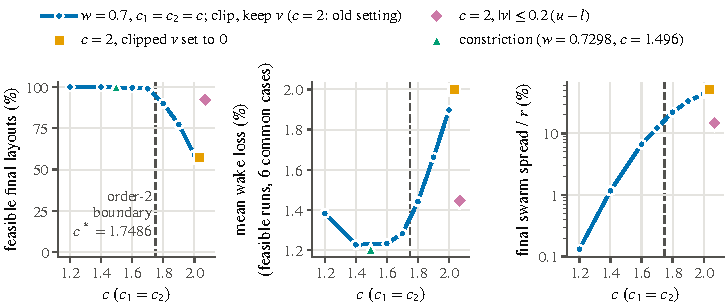
\includegraphics[width=\textwidth]{figures_mpce/csweep.pdf}
\caption{Stand-alone PSO with $w=0.7$ and $c_1=c_2=c$ on the 12 split cases $\times$ 30 seeds (6{,}030 evaluations, random starts; line with circles), the old setting ($c=2$) with two other bound-handling rules (clipped velocity components set to zero, squares; velocity clamping $|v|\le v_{\max}=0.2\,(u-l)$, diamonds; drawn slightly to the right of $c=2$), and the constriction setting (triangles; $w=0.7298$, $c=1.49618$; stored runs of the main comparison, spread not logged). The dashed vertical line is the order-2 stability boundary $c^\ast=12(1-w^2)/(7-5w)=1.7486$ of Proposition~\ref{prop:S-pso-stability} (stagnation, no bounds). Left: feasible final layouts (\% of 360 runs). Middle: mean wake loss of the feasible runs, averaged over the 6 cases in which every setting has at least 15 feasible runs. Right: median final swarm spread (mean over particles of the RMS turbine distance to the global best), relative to the farm radius (log scale). All settings start from the same seeded initial swarm. Values: Table~\ref{tab:S-csweep}.}
\label{fig:S-csweep}
\end{figure*}
\endgroup
\emph{Coefficient sweep.} A sweep of $c_1=c_2=c$ at $w=0.7$ (Fig.~\ref{fig:S-csweep} and Table~\ref{S-tab:S-csweep}; 360 runs per setting; $c=2.0$ reproduces the stored old-setting runs bit for bit) shows that the boundary $c^\ast=1.7486$ marks approximately where this PSO starts to fail: at least 98.9\% of the runs are feasible for $c\le1.7$, then feasibility declines progressively (90.0\% at $c=1.8$, 58.9\% at 2.0); velocity clamping raises it to 92.2\%, still worse than constriction in all 12 cases.
% CHECK-CSWEEP [S01] c = 2.0 reproduces the stored old-setting runs; [S02] c <= 1.7 >= 98 % feasible; [S03] c = 1.8 > 1.9 > 2.0; [S04] decline starts in the step containing c*; [S05] progressive, no jump; [S10] vmax >= 90 %; [S11] vmax worse than constriction in all 12 cases (never "causes")
There is no step at $c^\ast$: the decline begins between 1.7 and 1.8 and accelerates, while the swarm spread grows smoothly with $c$ (by about an order of magnitude from $c=1.4$ to 1.7) and the wake loss rises already on the stable side (lower at $c=1.6$ than at 1.7 in 10 of 12 cases, $p=0.005$), then in all 12 cases from 1.7 to 1.8. The boundary marks where the steps become too large for this bounded problem; the sweep does not show that crossing it causes the failure.
% CHECK-CSWEEP [S06] spread grows monotonically, >= 5x from 1.4 to 1.7; [S07] loss degrades on the stable side, c = 1.6 beats 1.7 in >= 10 of 12 (Wilcoxon p < 0.05); [S08] 1.7 -> 1.8 worsens the loss in all 12 cases
Zeroing clipped velocity components does not rescue the old setting (57.2\% feasible), whereas clamping brings it to about the level of $c=1.8$: the deficit comes mainly from the large steps, not from the bound handling.
% CHECK-CSWEEP [S09] zeroing clipped velocities no rescue; [S12] vmax indistinguishable from c = 1.8

Table~\ref{tab:baseline} shows the effect on a comparison. It ranks an eight-method pool, the methods of Table~\ref{tab:friedman68} with LX-SSA-VNS instead of PSO-VNS, once with each PSO setting (all other methods use identical runs): with the old setting, SSA-VNS ranks first and PSO only in position 5, behind both salp-swarm hybrids; with the constriction setting, PSO ranks first, ahead of every salp-swarm method (standard coefficients~\cite{Clerc2002}; none of the methods was tuned on these cases). The reversal holds at 6,030 evaluations; on the six largest cases at 120,030, SSA-VNS ranks ahead of PSO (4.17 vs.\ 5.83; Section~\ref{sec:budget}). The old setting thus makes the methods compared with it, including LX-SSA~\cite{Solanki2023}, appear stronger than they are.
% CHECK-FINAL [C27]: same pool: old setting SSA-VNS (1.99) and LX-SSA-VNS (2.65) ahead of PSO (5.04, NBaseOldPSOPos); constriction PSO ahead of every salp-swarm method (NBaseNewBest = PSO)
% CHECK-FINAL [C45]: at 120,030 evaluations SSA-VNS ranks ahead of PSO on the six largest cases

\subsection{Overall Comparison}
\label{sec:overall}
% >>>>> begin analysis/mpce_tab_friedman68.tex
%% generated by mpce_results.py -- do not edit by hand
\begin{table}[!t]
\centering
\caption{Case-level analysis of the eight methods over the 68 benchmark cases.}
\label{tab:friedman68}
\scriptsize\setlength{\tabcolsep}{2pt}
\begin{tabular}{lcccccc}
\toprule
Method & Avg.\ rank & Best & Feas. & $p_z$ & $p_W$ & $\overline{\Delta L}$ \\
\midrule
PSO-VNS & 1.82 & 29 & 100.0 & -- & -- & -- \\
PSO & 1.97 & 25 & 100.0 & 0.713 & 0.296 & $-0.018$ \\
SSA-VNS & 3.45 & 0 & 99.6 & $2.0\times10^{-4}$ & $5.7\times10^{-11}$ & $-0.330$ \\
VNS & 4.40 & 3 & 100.0 & $2.4\times10^{-9}$ & $1.3\times10^{-10}$ & $-0.465$ \\
SSA & 5.38 & 0 & 97.6 & $8.3\times10^{-17}$ & $4.5\times10^{-11}$ & $-0.611$ \\
MS-SLSQP & 5.88 & 1 & 100.0 & $1.8\times10^{-21}$ & $4.2\times10^{-11}$ & $-0.435$ \\
LX-SSA & 6.06 & 0 & 96.9 & $3.3\times10^{-23}$ & $4.5\times10^{-11}$ & $-0.765$ \\
DE & 7.04 & 0 & 71.4 & $1.0\times10^{-34}$ & $5.6\times10^{-11}$ & $-0.887$ \\
\bottomrule
\end{tabular}
\par\vspace{2pt}\parbox{\columnwidth}{\scriptsize Avg.\ rank: average rank of the mean feasible objective, i.e., conditional quality subject to qualification, not reliability (1 = best; fewer than 15 feasible runs in a case = ranked below the qualified methods, by number of feasible runs); Best: cases in which the method alone ranks first; Feas.: feasible runs (\%); $p_z$: Holm-adjusted $p$ of the average-rank test against PSO-VNS. Because mean-rank tests depend on the pool~\cite{Benavoli2016}, $p_W$ gives the primary test, the two-sided Wilcoxon signed-rank test on the 68 per-case mean wake losses (Holm-adjusted over the 7 methods) and $\overline{\Delta L}$ the mean wake-loss difference (pp, PSO-VNS minus method; negative = PSO-VNS better) over the cases in which both methods have at least 15 feasible runs (66 for SSA, 66 for LX-SSA, 50 for DE, otherwise 68). Friedman $\chi^2_F=319.3$ (7 d.f.), $p=4.6\times10^{-65}$; Iman--Davenport $F_F=136.5$ (7, 469 d.f.), $p=6.7\times10^{-109}$.}
\end{table}
% <<<<< end analysis/mpce_tab_friedman68.tex
% >>>>> begin analysis/mpce_tab_wtl.tex
%% generated by mpce_results.py -- do not edit by hand
\begin{table}[!t]
\centering
\caption{Run-level outcome of PSO-VNS against each method (W/T/L over the 68 cases).}
\label{tab:wtl}
\scriptsize\setlength{\tabcolsep}{1.6pt}
\begin{tabular}{llcccccccc}
\toprule
DS & $r$ (m) & Cases & PSO & \begin{tabular}{@{}c@{}}SSA-\\VNS\end{tabular} & SSA & \begin{tabular}{@{}c@{}}LX-\\SSA\end{tabular} & DE & VNS & \begin{tabular}{@{}c@{}}MS-\\SLSQP\end{tabular} \\
\midrule
I & 500 & 9 & 0/8/1 & 6/3/0 & 8/1/0 & 8/1/0 & 7/2/0 & 6/3/0 & 7/2/0 \\
I & 750 & 11 & 1/8/2 & 9/2/0 & 10/1/0 & 10/1/0 & 9/2/0 & 8/3/0 & 10/1/0 \\
I & 1000 & 14 & 3/11/0 & 9/5/0 & 12/2/0 & 12/2/0 & 12/2/0 & 12/2/0 & 12/2/0 \\
II & 500 & 9 & 3/5/1 & 7/2/0 & 7/2/0 & 8/1/0 & 7/2/0 & 7/1/1 & 8/1/0 \\
II & 750 & 11 & 2/9/0 & 8/3/0 & 10/1/0 & 10/1/0 & 9/2/0 & 8/3/0 & 9/2/0 \\
II & 1000 & 14 & 5/9/0 & 10/4/0 & 12/2/0 & 12/2/0 & 12/2/0 & 10/4/0 & 13/1/0 \\
\midrule
All & & 68 & 14/50/4 & 49/19/0 & 59/9/0 & 60/8/0 & 56/12/0 & 51/16/1 & 59/9/0 \\
$\tilde r_{\rm rb}$ & & & +0.08 & +0.72 & +0.98 & +0.97 & +1.00 & +0.84 & +0.99 \\
\bottomrule
\end{tabular}
\par\vspace{2pt}\parbox{\columnwidth}{\scriptsize W/T/L: cases in which PSO-VNS is significantly better / not different / worse (two-sided Wilcoxon signed-rank test on 30 seed-paired runs, $\alpha=0.05$, Holm-adjusted over the seven comparisons of PSO-VNS in each case, a different family from Table~\ref{tab:ablation}; an infeasible run ranks below every feasible run). $\tilde r_{\rm rb}$: median rank-biserial correlation (positive = PSO-VNS better; zero differences dropped, $r_{\rm rb}=0$ if all are zero).}
\end{table}
% <<<<< end analysis/mpce_tab_wtl.tex

\begin{table}[!t]
\centering\footnotesize
\caption{Expanded nine-method benchmark pool. Eight-method results remain a separate analysis.}
\label{tab:ga-main}
\begin{tabular}{lcccc}\toprule
Method & Avg. rank & Best & Feas. (\%) & $p_W$ vs. GA \\\midrule
PSO-VNS & \textbf{2.18} & \textbf{21} & 100.0 & 0.101 \\
PSO & 2.40 & 17 & 100.0 & 0.696 \\
GA & 2.74 & 16 & 98.6 & -- \\
SSA-VNS & 4.32 & 0 & 99.6 & $9.29\times10^{-10}$ \\
VNS & 5.21 & 3 & 100.0 & $1.07\times10^{-9}$ \\
SSA & 6.34 & 0 & 97.6 & $6.06\times10^{-11}$ \\
MS-SLSQP & 6.85 & 1 & 100.0 & $2.34\times10^{-10}$ \\
LX-SSA & 7.01 & 0 & 96.9 & $6.06\times10^{-11}$ \\
DE & 7.96 & 0 & 71.4 & $1.14\times10^{-10}$ \\
\bottomrule\end{tabular}
\par\vspace{3pt}\parbox{\linewidth}{\footnotesize 68 cases, 30 paired seeds, 6,030 evaluations. Best: cases won outright; bold: best method. $p_W$: Holm-adjusted case-mean Wilcoxon comparison with GA. Qualification and conditional quality follow Section~\ref{sec:setup-stats}; ranks depend on the method pool. Source: Table~\ref{S-tab:S-xp-ga}.}
\end{table}

Over the eight methods (Table~\ref{tab:friedman68}), the Friedman test rejects the hypothesis of equal performance ($\chi^2_F=319.3$, $p=\ensuremath {4.6\times 10^{-65}}$; Iman--Davenport $F_F=136.5$, $p=\ensuremath {6.7\times 10^{-109}}$). PSO-VNS has the best average rank (1.82), alone ranks first in 29 cases, and stays first when the final layouts are re-evaluated with 5$^\circ$ or 1$^\circ$ direction sub-bins (1$^\circ$: 2.09; Section~\ref{sec:robustness}). In the Holm-adjusted post hoc tests ($p_z$ in Table~\ref{tab:friedman68}; tied ranks make them conservative), PSO-VNS ranks significantly better than SSA-VNS, VNS, SSA, MS-SLSQP, LX-SSA and DE, but not than PSO ($p_{\rm Holm}=0.71$). The rank order and these conclusions are unchanged for thresholds of 1, 10, 15, 20, 25 and 30 feasible runs; significant comparisons with PSO-VNS favor the same method in each of the six clusters, and leaving out one cluster changes none of them (Tables~\ref{S-tab:X-threshold}--\ref{S-tab:X-loco}). The real-coded GA (Section~\ref{sec:setup-cases}) does not change this picture (Table~\ref{tab:ga-main}; details: Table~\ref{S-tab:S-xp-ga}): in the nine-method pool it ranks third (2.74, against 2.18 for PSO-VNS and 2.40 for PSO; Holm $p=0.47$ against either), and it is practically equivalent to PSO at the case level (GA $-$ PSO: $+0.008$~pp, 90\% CI [$-$0.022, 0.041]), whereas its interval against PSO-VNS, [$-$0.006, 0.062]~pp, extends beyond the margin. Its leads at the sites are reported in Sections~\ref{sec:hornsrev-site} and~\ref{sec:iea37}.
% CHECK-FINAL [C01]: main.friedman.best_ranked == PSOBV; [C02]: p < 0.05 (verb generated: \NFriedVerb); [C03]: p_holm_vs_focus: only PSOC >= 0.05
% CHECK-DIR [F06]: PSO-VNS best average rank with 5-deg and 1-deg sub-bins (\NFRankPSOVNSOne)
% CHECK-EXTRA [X02][X03][X05]-[X09] six thresholds 1-30; [X11] clusters 6/6 same direction for comparisons with PSO-VNS; [X14] LOCO changes only \NXLocoChanged (not a PSO-VNS comparison), PSO-VNS always best

% Page budget: the rank chart stays in the supplementary material (Fig. S-fig:S-ranks); the main-text version was:
% \begin{figure}[!t]
% \centering
% \pipefig{0.4\textwidth}{figures_mpce/avg_ranks.pdf}{5cm}
% \caption{Average rank of the eight methods of the main comparison over the 68 benchmark cases (feasibility-aware ranking of Table~\ref{tab:friedman68}; 1 = best).}
% \label{fig:ranks}
% \end{figure}
% CHECK (pipeline): avg_ranks.pdf is drawn from the same ranks as tab:friedman68 (\NRankPSOVNS ... \NRankDE)
In Fig.~\ref{S-fig:S-ranks}, the two PSO-based methods lead with a small gap, far ahead of SSA-VNS; both hybrids rank ahead of their first phase and of VNS, and the last rank of DE also reflects its feasibility (71.4\% of its runs). Figs.~\ref{S-fig:S-box-max} and~\ref{S-fig:S-box-mid} show the distributions of the feasible runs for the largest and the middle $N$ of each farm.
% CHECK (pipeline): rank values from tab:friedman68; [C01] PSO-VNS best; DE feasibility \NFeasDE (CHECK-FINAL [C08])

Against SSA-VNS, PSO-VNS is significantly better in 49 cases and never worse ($p_{\rm Holm}=\ensuremath {5.7\times 10^{-11}}$). Against SSA, LX-SSA, DE, VNS and MS-SLSQP (untuned DE; finite-difference gradients), it is significantly better in most cases; it is never significantly worse than SSA-VNS, SSA, LX-SSA, DE and MS-SLSQP and significantly worse than VNS in one case. On the all-run paired outcome, too, PSO-VNS is better than each of these six methods (Section~\ref{sec:archive-reliability}). PSO-VNS is more reliable in reaching feasibility on the Horns Rev~1 block with random starts (30/30 vs.\ 19/30, McNemar $p=\ensuremath {9.8\times 10^{-4}}$; Section~\ref{sec:hornsrev-site}) and ranks best on the six largest cases at all three budgets (exploratory; Section~\ref{sec:budget}). The leading methods depend on the conditions: from feasible starts, VNS ranks first (Section~\ref{sec:feasinit}); under the Gaussian wake, PSO ranks narrowly ahead of PSO-VNS with 15$^\circ$ bins but not with 1$^\circ$ sub-bins (Section~\ref{sec:gaussian}).
% CHECK (manual, 2026-10-04): all-run scores of PSO-VNS 0.734 (SSA-VNS) ... 0.897 (DE), case CIs lower limits >= 0.700 (analysis/rev3_inference.json, tab:S-sa-allrun); order by score SSA-VNS, VNS, MS-SLSQP, SSA, LX-SSA, DE
% CHECK-FINAL [C06]: wtl.SSABV.L == 0; [C07]: better than SSA, LX-SSA, DE, VNS, MS-SLSQP in most cases; [C08]/[C20]: Horns Rev PSO-VNS 30/30, PSO < 30/30; [C29]: six largest cases best at all budgets; [C28]: feasible-start BVNS best; [C22]: Gauss 15 deg PSOC first, PSOBV second
% CHECK-EXTRA [X52] McNemar (one site, random starts); CHECK-DIR [F06] best rank 15/5/1 deg; [F09] Gaussian: PSO first at 15 deg, PSO-VNS at 1 deg

\begin{figure*}[!t]
\centering
\pipefig{0.72\textwidth}{figures_mpce/wakeloss_vs_n.pdf}{8cm}
\caption{Mean wake loss (\% of the wake-free benchmark objective) of the feasible runs versus the prescribed number of turbines $N$, for each farm and wind data set (30 runs of 6,030 evaluations, random initialization). A point is drawn only when the method has at least 15 feasible runs in that case, so a curve (mostly DE) stops where the method has too few feasible runs.}
\label{fig:wakeloss}
\end{figure*}
The wake loss grows with $N$, falls as the farm becomes larger, and is higher for the broader wind rose of Data Set~II (Fig.~\ref{fig:wakeloss}). PSO-VNS ends feasible in all runs (DE: 71.4\%). In the densest cases (500~m, $N=10$), the global best of the PSO phase is feasible at the switch in only 63.3\% of the runs, but all runs are feasible after the VNS phase.
% CHECK-FINAL [C42]: case-mean wake loss grows with N, falls with r, DS II >= DS I; [C08]: feasible_pct.PSOBV == 100; [C24]: dense_500_10 feasible at switch < 100
For the smallest $N$, all methods reach almost no wake loss, so these cases cannot separate the methods; the curves fan out with $N$, most in the small farm and under the broad rose of Data Set~II.
% CHECK-FINAL [C42] (monotone in N, r, data set); curves: wakeloss_vs_n.pdf from the case means of tab:friedman68 runs

\begin{figure*}[!t]
\centering
\pipefig{0.7\textwidth}{figures_mpce/ablation_convergence.pdf}{6.6cm}
\caption{Convergence of the nine component-analysis variants (Table~\ref{tab:ablation}) for the largest turbine count of each farm: median best feasible wake loss over 30 runs versus evaluations. PSO-VNS and PSO coincide up to 3,030 evaluations (dotted line), where PSO-VNS switches to VNS. Curves of the main comparison: Fig.~\ref{S-fig:S-conv-max} of the supplementary material.}
\label{fig:conv-max}
\label{fig:ablation}
\end{figure*}
% CHECK (pipeline count): \NAblNVar = variants of tab:ablation = curves of ablation_convergence.pdf; [C58] ranks

After the switch, both keep improving (Fig.~\ref{fig:conv-max}): the VNS phase removes on average 30.3\% (median 22.6\%) of the wake loss left after the PSO phase and repairs 26 runs infeasible at the switch, whereas continuing PSO for the same 3,000 evaluations removes 29.2\% (median 20.6\%).
% CHECK-FINAL [C10]: phase2 PSOBV.mean >= PSOC_continued.mean > 0 ("both keep improving")

\subsection{PSO-VNS versus PSO}
\label{sec:psovns-pso}
Against PSO, PSO-VNS is significantly better in 14 cases, tied in 50 and worse in 4 (run level, Table~\ref{tab:wtl}). The case means do not differ significantly ($\overline{\Delta L}=\ensuremath {-}0.018$~pp, $p=0.30$; Hodges--Lehmann estimate \ensuremath {-}0.003~pp). Whether the difference is negligible at the post hoc margin $\pm0.05$~pp, a primary question (Section~\ref{sec:setup-stats}), depends on the level of inference (Table~\ref{tab:equiv-main}; all pairs: Table~\ref{S-tab:X-equiv-levels}): on this fixed benchmark (seed level, at which the verdict is decided), the two are equivalent, with a small significant advantage of PSO-VNS inside the margin (90\% CI [\ensuremath {-}0.026, \ensuremath {-}0.010]); under exchangeable-case sensitivity they are also equivalent ([\ensuremath {-}0.041, 0.004], TOST $p=0.011$; shifted-null check on this dataset, $p=0.015$; minimal margin 0.041); under the cluster-level sensitivity analysis (six scenario clusters), equivalence is not shown (CR2 [\ensuremath {-}0.067, 0.031], minimal margin 0.067). In the Bayesian signed-rank test, practical equivalence is the most probable outcome (posterior probability \ensuremath {>0.99}; posterior means 0.25/0.62/0.12 for PSO-VNS better by more than the margin/equivalent/PSO better). The margin corresponds to 4.1 (Data Set~I) and 2.1~MWh/yr (Data Set~II) per turbine, the mean gain of PSO-VNS to 0.2~MWh/yr per turbine (0.020\% of AEP). Spread and worst run do not differ ($p=0.55$, 0.80).
% CHECK-FINAL [C04]: PSOC: W >= L, mean loss PSOBV < PSOC, case-mean p >= 0.05; [C49]: case-level 90% CI inside +-m, P(rope most probable) printed via \NBayPSOVNSvsPSORope; [C52]: SD p and worst-run p >= 0.05
% CHECK-EXTRA [X39] seed and case level equivalent, cluster level not; [X40] seed-level CI excludes 0 inside m; [X41] minimal margins seed < case < m < cluster; [X48] Bayesian wording + posterior means; [X50] HL near 0; [X56] margin 4.1/2.1 MWh/yr per turbine, mean gain 0.2; [X25] energy < 0.05 % AEP

\begingroup\swResRefs
%
% --- tab:X-equiv-levels and tab:equivalence (all 18 pairs) moved to the supplementary material; compact main-text summary:
\begin{table}[!t]
\centering
\caption{Primary equivalence questions and sampling-control contrasts (68 cases, 6,030 evaluations, 15$^\circ$ rose unless stated; margin $m=0.05$~pp, a post hoc convention). $\overline{\Delta L}$: mean case-mean wake-loss difference, first minus second method (pp; negative = first better). 90\% intervals at the three levels of Definition~\ref{def:S-equiv}: seed (fixed benchmark; the level at which verdicts are decided), case (exchangeable-case sensitivity) and cluster (benchmark-group sensitivity; CR2, six scenario clusters, 5 d.f.). Verdict by interval inclusion at $\pm m$: E, equivalent; NS, a gain of the first method larger than $m$ is ruled out (non-superiority); G, first method better by more than $m$; --, inconclusive. $P_{\rm rope}$: share of Bayesian signed-rank posterior samples in which practical equivalence is the most probable outcome (not the probability that $\Delta$ lies within $\pm m$). All 18 pairs, TOST $p$ values and minimal margins: Tables~\ref{S-tab:X-equiv-levels} and~\ref{S-tab:equivalence}.}
\label{tab:equiv-main}
\scriptsize\setlength{\tabcolsep}{2pt}
\begin{tabular}{@{}lcccccc@{}}
\toprule
Pair (first vs.\ second) & $\overline{\Delta L}$ & Seed 90\% CI & Case 90\% CI & Cluster 90\% CI & Verdict$^{b}$ & $P_{\rm rope}$ \\
\midrule
\multicolumn{7}{@{}l}{\emph{Primary}} \\
PSO-VNS vs.\ PSO & $-0.018$ & [$-$0.026, $-$0.010] & [$-$0.041, 0.004] & [$-$0.067, 0.031] & E / E / -- & $>$0.99 \\
\quad 1$^\circ$ re-evaluation$^{a}$ & $-0.043$ & n/r & [$-$0.062, $-$0.025] & n/r & n/r / -- / n/r & n/r \\
SSA-VNS vs.\ RSD-VNS & $+0.024$ & [0.002, 0.046] & [$-$0.022, 0.062] & [$-$0.051, 0.099] & NS / NS / -- & 0.77 \\
\midrule
\multicolumn{7}{@{}l}{\emph{Exploratory: sampling controls}} \\
SSA-VNS vs.\ RS-VNS & $-0.068$ & [$-$0.092, $-$0.044] & [$-$0.101, $-$0.039] & [$-$0.126, $-$0.011] & -- / -- / -- & 0.70 \\
RSD-VNS vs.\ RS-VNS & $-0.093$ & [$-$0.115, $-$0.070] & [$-$0.127, $-$0.055] & [$-$0.131, $-$0.054] & G / G / G & 0.05 \\
LX-SSA-VNS vs.\ RSD-VNS & $+0.087$ & [0.065, 0.110] & [0.047, 0.126] & [0.004, 0.170] & NS / NS / NS & 0.10 \\
PSO-VNS vs.\ RSD-VNS & $-0.306$ & [$-$0.325, $-$0.287] & [$-$0.380, $-$0.239] & [$-$0.442, $-$0.171] & G / G / G & $<$0.01 \\
\bottomrule
\end{tabular}
\par\vspace{2pt}\parbox{\linewidth}{\scriptsize $^{a}$Stored 15$^\circ$ layouts re-evaluated with 1$^\circ$ sub-bins, not re-optimized (Section~\ref{sec:direction}; Table~\ref{S-tab:F-equiv}); n/r: not reported here. $^{b}$Seed / case / cluster level. SSA-VNS vs.\ RSD-VNS at the seed level is also inside $\pm m$ (not under joint seed resampling, Table~\ref{S-tab:S-sa-syncseed}); the primary question for this pair is one-sided.}
\end{table}

\begin{figure}[!t]
\centering
\pipefig{0.45\textwidth}{figures_mpce/equiv_curve.pdf}{5cm}
\caption{Equivalence curve of PSO-VNS vs.\ PSO: TOST $p$ value versus the equivalence margin $m$ (pp of wake loss) at three levels of inference (Table~\ref{tab:equiv-main}): seed level (fixed benchmark, at which verdicts are decided; bootstrap of the seed-paired runs within every case), case level (sensitivity; bootstrap over the 68 cases, as Table~\ref{S-tab:equivalence}) and cluster level (sensitivity; six farm clusters; CR2 cluster-robust $t$ with 5 d.f., solid, and the restricted wild-cluster bootstrap, dashed). Dotted lines: $\alpha=0.05$ and the margin $m=0.05$~pp. The dots mark the minimal margins $m_{\min}$, at which a curve crosses $\alpha$; equivalence holds at every margin to the right of the dot. The seed- and case-level bootstrap curves stop at their resolution limit $1/10{,}001$.}
\label{fig:equiv-curve}
\end{figure}
\endgroup
% CHECK-EXTRA [X57] equiv_curve.pdf generated in the same run; [X41] minimal margins seed < case < m < cluster
The minimal margin grows with the scope of the level (Definition~\ref{def:S-equiv}; none treats the cases as a sample of new farms); as the post hoc margin lies just above the case-level value, Fig.~\ref{fig:equiv-curve} gives the whole TOST curve. The seed-level interval excludes zero: the methods differ reproducibly here, but by less than the margin. The all-run paired outcome, a separate endpoint that counts wins rather than measuring their size, also favors PSO-VNS (Section~\ref{sec:archive-reliability}). No pair is equivalent at the cluster level.
% CHECK (manual, 2026-10-04): all-run PSO-VNS vs PSO W/T/L 950/348/742, score 0.551, case CI [0.516, 0.587], two-stage [0.511, 0.591], Holm sign p 4.7e-7 (analysis/rev3_inference.json, tab:S-sa-allrun); calibrated case-level p_- 0.015 (tab:S-sa-tostaudit)
% CHECK-EXTRA [X39]-[X41]; [X55] no pair equivalent at the cluster level; main-comparison pairs other than PSO: whole 90% CI beyond -m at all three levels (tab:X-equiv-levels, m_min > m)

\begingroup\swResRefs\swResWrapNotes
% Page budget: kept in the supplementary material: \SuppTable{tab:X-heterogeneity}
\endgroup
The average hides case-level differences in both directions: 11 cases favor PSO-VNS by more than the margin (by up to 0.41~pp) and 8 favor PSO (up to 0.27~pp; Table~\ref{S-tab:X-heterogeneity}). The two are equivalent for $N<10$ (48 cases, 90\% CI [\ensuremath {-}0.005, 0.021]) but not for $N\ge10$ (\ensuremath {-}0.079~pp, [\ensuremath {-}0.142, \ensuremath {-}0.017]) or on the 44 cases with a wake loss of at least 0.2~pp ([\ensuremath {-}0.060, 0.008]). They follow a data set $\times$ density crossover (density $\phi=\ensuremath {N\,(\ell _{\min }/2r)^2}$; post hoc, exploratory; interaction $p=0.01$): as $\phi$ grows, PSO-VNS gains in Data Set~II (slope \ensuremath {-}0.52~pp, $p=\ensuremath {1.0\times 10^{-4}}$) and PSO in Data Set~I (+0.29~pp, $p=0.0012$). In the post hoc subgroup Data Set~II, $N\ge10$, PSO-VNS has the lower mean wake loss in 10 of 10 cases ($p_{\rm Holm}\le0.018$ over all 28 case-mean Wilcoxon tests; 0.221\% of AEP); all 7 Data Set~I cases beyond the margin favor PSO. Re-evaluated with 1$^\circ$ sub-bins, PSO-VNS is slightly but significantly better than PSO ($\overline{\Delta L}=\ensuremath {-}0.043$~pp, 90\% CI [\ensuremath {-}0.062, \ensuremath {-}0.025]; Table~\ref{S-tab:F-equiv}); optimized directly with 1$^\circ$ bins (eight cases), it gains $-0.194$~pp, beyond the margin, against $-0.086$~pp in a seed-matched control arm optimized with 15$^\circ$ bins and evaluated with 1$^\circ$ bins (Section~\ref{sec:direction}).
% CHECK-EXTRA [X43] 11/8 beyond +-m, max 0.41/0.27; [X44] N < 10 equivalent, N >= 10 not; [X45] non-trivial cases not equivalent; [X47] data set x density crossover (exploratory, post hoc); [X19] DS II N >= 10 survives all-family Holm ("<=", R5 O13); [X27] DS II N >= 10 ~0.2 % AEP
% CHECK-FINAL [C32]: DS II N >= 10 case-mean wins > losses
% CHECK-DIR [F10]: 1-deg PSO-VNS - PSO CI below 0, not equivalent; [F14]: DS II N >= 10 advantage survives at 1 deg

The average verdict thus depends on the case mix: in the 24 cases with a PSO-VNS wake loss below 0.2~pp, both find almost wake-free layouts and none differs by more than the margin. The differences are structured (3 of 6 cluster means beyond the margin, in both directions): in Data Set~II, 11 cases beyond the margin, the larger layouts of all three farms, favor PSO-VNS, and in Data Set~I all 7, dense layouts in the two smaller farms, favor PSO (Table~\ref{S-tab:X-beyond}). The crossover, found post hoc with no cause identified, is a hypothesis for designed experiments. PSO-VNS thus does not dominate a well-configured PSO: it is at least as good on average, gains in larger Data Set~II layouts and loses in dense Data Set~I layouts.
% CHECK-EXTRA [X44] N < 10 (48 cases) equivalent; [X45] trivial cases equivalent, every case beyond the margin non-trivial, non-trivial not equivalent; [X46] 3 of 6 cluster means beyond +-m in opposite directions (2 PSO-VNS, 1 PSO; DS I 500 m, DS II 1000 m); [X47] DS I cases beyond the margin all favor PSO and are dense, DS II 11 favor PSO-VNS, 1 favors PSO (exploratory, post hoc)

% end optA/sw/06_results.tex

% begin optA/sw/07_ablation.tex
\section{Component Analysis of Two-Phase Hybrids}
\label{sec:ablation}
% SWEVO extension: the generated tables tab:D-vns and tab:D-rsreplay are captured from analysis/mpce_supp_diag.tex (its
% figure fig:D-psodyn is discarded here, not placed); tab:switch and tab:equivalence come from the global capture of
% analysis/mpce_supplementary.tex, tab:split from analysis/mpce_tab_split.tex (all logged in optA/sw/moved.md)
\begingroup\RenewEnviron{figure*}[1][]{}\endgroup% [flattened: removed \CaptureSuppTables{analysis/mpce_supp_diag.tex}]
% [flattened: removed \CaptureSuppTables{analysis/mpce_tab_split.tex}]
\makeatletter
% \AblTable[<placement>]{<label>}: like \SuppTable (placed once, TBD box if absent), with a placement of our choice
\newcommand{\AblTable}[2][!t]{\@ifundefined{supp@body@#2}{\SuppTable{#2}}{\@ifundefined{supp@used@#2}{%
  \global\@namedef{supp@used@#2}{}\begin{table}[#1]\@nameuse{supp@body@#2}\end{table}}{}}}
% posterior probabilities in math mode: "= value", or "< 0.01" / "> 0.99" for a bound (rule of \BayEq in the supplement)
\newcommand{\AblBayEq}[1]{\expandafter\abl@bayeq#1\@nil}
\def\abl@bayeq#1#2\@nil{\ifx#1\ensuremath #2\else =#1#2\fi}
\makeatother
% >>>>> begin analysis/mpce_tab_ablation.tex
%% generated by mpce_results.py -- do not edit by hand
\begin{table}[!t]
\centering
\caption{Component analysis over the 68 benchmark cases (6,030 evaluations, 30 seed-paired runs).}
\label{tab:ablation}
\scriptsize\setlength{\tabcolsep}{2.5pt}
\begin{tabular}{lcccc}
\toprule
Variant & Phase 1 & Phase 2 & Avg.\ rank & Feas.\ (\%) \\
\midrule
PSO-VNS & PSO & VNS & 1.96 & 100.0 \\
SSA-VNS & SSA & VNS & 4.46 & 99.6 \\
LX-SSA-VNS & LX-SSA & VNS & 5.41 & 99.9 \\
RS-VNS & random (square) & VNS & 5.29 & 99.4 \\
RSD-VNS & random (disc) & VNS & 3.77 & 99.8 \\
VNS & -- & VNS & 6.12 & 100.0 \\
PSO & PSO & -- & 2.24 & 100.0 \\
SSA & SSA & -- & 7.50 & 97.6 \\
LX-SSA & LX-SSA & -- & 8.25 & 96.9 \\
\bottomrule
\end{tabular}

\smallskip
\begin{tabular}{l>{\raggedright\arraybackslash}p{1.95cm}ccc}
\toprule
Contrast & Isolates & W/T/L & $p_W$ & $\overline{\Delta L}$ \\
\midrule
PSO-VNS vs.\ PSO & VNS phase (PSO) & 8/58/2 & 0.592 & $-0.018$ \\
SSA-VNS vs.\ SSA & VNS phase (SSA) & 39/29/0 & $5.7\times10^{-10}$ & $-0.294$ \\
LX-SSA-VNS vs.\ LX-SSA & VNS phase (LX-SSA) & 34/34/0 & $1.1\times10^{-10}$ & $-0.394$ \\
PSO-VNS vs.\ VNS & swarm start vs.\ best initial point & 49/18/1 & $5.7\times10^{-10}$ & $-0.465$ \\
PSO-VNS vs.\ RS-VNS & PSO vs.\ random sampling & 47/21/0 & $3.2\times10^{-10}$ & $-0.399$ \\
SSA-VNS vs.\ RS-VNS & SSA vs.\ random sampling & 2/66/0 & 0.002 & $-0.068$ \\
LX-SSA-VNS vs.\ RS-VNS & LX-SSA vs.\ random sampling & 1/67/0 & 0.718 & $-0.005$ \\
PSO-VNS vs.\ RSD-VNS & PSO vs.\ disc sampling & 45/23/0 & $4.0\times10^{-10}$ & $-0.306$ \\
SSA-VNS vs.\ RSD-VNS & SSA vs.\ disc sampling & 0/66/2 & 0.014 & $+0.024$ \\
LX-SSA-VNS vs.\ RSD-VNS & LX-SSA vs.\ disc sampling & 1/62/5 & $8.2\times10^{-6}$ & $+0.087$ \\
RSD-VNS vs.\ RS-VNS & disc vs.\ square sampling & 6/62/0 & $4.2\times10^{-7}$ & $-0.093$ \\
PSO-VNS vs.\ SSA-VNS & PSO vs.\ SSA as Phase~1 & 44/24/0 & $2.5\times10^{-10}$ & $-0.330$ \\
PSO-VNS vs.\ LX-SSA-VNS & PSO vs.\ LX-SSA as Phase~1 & 47/21/0 & $2.3\times10^{-10}$ & $-0.393$ \\
SSA-VNS vs.\ LX-SSA-VNS & LX-SSA as published (hybrid) & 2/66/0 & $2.7\times10^{-5}$ & $-0.063$ \\
LX-SSA vs.\ SSA & LX-SSA as published (alone) & 0/64/4 & $1.3\times10^{-6}$ & $+0.153$ \\
\bottomrule
\end{tabular}
\par\vspace{2pt}\parbox{\columnwidth}{\scriptsize Top: average rank among the nine variants (Friedman $\chi^2_F=374.3$, 8 d.f., $p=5.96\times10^{-76}$) and feasible runs. Bottom: planned contrasts. W/T/L: cases in which the first variant is significantly better / not different / worse (run-level Wilcoxon, $\alpha=0.05$, Holm-adjusted over the fifteen contrasts of each case, a different family from Table~\ref{tab:wtl}); $p_W$: Wilcoxon test on the 68 per-case mean wake losses, Holm-adjusted over the fifteen contrasts; $\overline{\Delta L}$: mean difference of the case-mean wake losses (pp; negative = first variant better) over the cases in which both variants have at least 15 feasible runs (66--68 of 68 per contrast).}
\end{table}
% <<<<< end analysis/mpce_tab_ablation.tex

The variants of Table~\ref{tab:ablation} combine a Phase~1 (PSO, SSA, LX-SSA, random sampling or none) with or without the same VNS phase (6,030 evaluations from random starts, same seeds; convergence: Fig.~\ref{fig:ablation}); their average ranks differ (Friedman $p=\ensuremath {6.0\times 10^{-76}}$). W/T/L, $p$ (Holm-adjusted Wilcoxon test on the 68 case means) and $\overline{\Delta L}$ (mean difference of the case means, pp) are those of Table~\ref{tab:ablation}; a 90\% bootstrap interval of $\overline{\Delta L}$ (in brackets) inside $\pm0.05$~pp means practical equivalence at the case level.
% CHECK-FINAL [C36]: Friedman rejects equal average ranks (\NAblP); pipeline-generated counts \NAblNContrasts (Holm family of each case), \NAblDf d.f., \NAblNVar variants in the caption. All DL in this section are \NCm...DL = tab:ablation values (R1-7, R5-F1)


\subsection{The VNS Phase}
\label{sec:abl-vns}
The VNS phase improves both salp-swarm methods: SSA-VNS is 39/29/0 (W/T/L) against SSA and LX-SSA-VNS 34/34/0 against LX-SSA ($\overline{\Delta L}=\ensuremath {-}0.294$ and \ensuremath {-}0.394). For PSO, which PSO-VNS repeats for its first 3,030 evaluations (Section~\ref{sec:hybrid}), the difference is small, not significant ($p=0.59$) and practically equivalent to zero at the case level (Section~\ref{sec:psovns-pso}). At this budget the VNS phase is essentially one compass-search descent: for PSO-VNS, the shake-and-search cycles take 21.5\% of the Phase-2 evaluations (pooled; median run 4.7\%) but give 0.5\% of the Phase-2 gain (2.5\% with the cycle cut off by the budget), and the median run with $N\ge12$ never shakes (Table~\ref{S-tab:D-vns}). The analysis thus measures the value of a local-search phase.
% CHECK-FINAL [C33]: VNS phase significant for SSA and LX-SSA (W > L, L = 0; case-mean p < 0.05, DL < 0), not for PSO (case-mean p >= 0.05, so also Holm); [C13]: PSOBV-PSOC W > L; [C49]: case-level 90 % CI \NEqPSOVNSvsPSOCI inside +-\NEqMargin
% CHECK-DIAG [D20]: cycles >= 15 % of the Phase-2 evaluations, < 5 % of the gain incl. the cut-off cycle, accepted cycles < 1 % (\NDCycleEvalsPctPSOVNS, median run \NDCycleEvalsPctMedianPSOVNS, \NDCycleSharePSOVNS, \NDCycleAllSharePSOVNS); [D08]: essentially one descent; [D09]: median run has no shaking step for N >= 12

% Page budget: kept in the supplementary material: \AblTable{tab:D-vns}
In Table~\ref{S-tab:D-vns} (12 split cases $\times$ 10 seeds), the first descent from the switch point takes a median of 2{,}860 evaluations in PSO-VNS and gives 97.5\% of the Phase-2 improvement (SSA-VNS 90.3\%, RS-VNS 88.6\%). A shake costs one evaluation, but the new descent after it scans $2n=4N$ moves per step, and 114 of 120 runs accept no cycle; accepted cycles use only $k=1$. For $N\ge12$ the first descent is unfinished in 39 of 40 runs, so the local-minimality guarantee (Proposition~\ref{S-prop:S-ls}) does not apply there. VNS never makes a feasible incumbent infeasible and starts from the best feasible Phase-1 layout when one exists. The contrasts thus test a truncated compass search after Phase~1; shaking and neighborhood change can matter only for small $N$.
% CHECK-DIAG [D08]: median shaking steps <= 2, >= 85 % of the Phase-2 improvement from the first descent for PSO-VNS, SSA-VNS, RS-VNS (\NDDescentSharePSOVNS, \NDDescentShareSSAVNS, \NDDescentShareRSVNS); no accepted cycle in \NDNoAcceptedPSOVNS of 120 runs; [D10]: accepted cycles only with k = 1; [D09]: N >= 12 first descent unfinished (\NDDescentUnfinishedLargePSOVNS of \NDRunsLargePSOVNS); [D11]: VNS never turns a feasible incumbent infeasible; [D12]: start = best feasible Phase-1 layout whenever Phase 1 evaluated one; [D20]: cycles costly relative to their gain

\subsection{Random-Sampling Controls}
\label{sec:abl-controls}
Random sampling of equal cost replaces Phase~1, uniform in the site disc (RSD-VNS) or in its bounding square (RS-VNS); VNS alone is a third control. RS-VNS is weak: 730 of its runs draw no feasible sample, although all of them draw samples wholly inside the circle; the spacing constraint is binding, and disc sampling rescues only 242 of these runs. RSD-VNS beats RS-VNS (6/62/0, $\overline{\Delta L}=\ensuremath {-}0.093$) and ranks third (3.77).
% CHECK-FINAL [C60]: RS-VNS runs without a feasible sample (\NRSRunsNoFeasSample) = rescued by disc sampling (\NRsSquareExplains) + none either way (\NRsSpacingDominates), rescued < none; LEAD: extend C60 with runs_no_feasible_but_inside_sample == runs_no_feasible_sample (\NRsNoFeasInside = \NRSRunsNoFeasSample, mpce_results.py phase1_replay.RSVNS) for "all of them"
% CHECK-FINAL [C57]: RSDVNS-RSVNS L == 0, W > 0, case-mean p_Holm < 0.05, DL < 0; [C58]: RSD-VNS ranks third of \NAblNVar

% Page budget: kept in the supplementary material: \AblTable{tab:D-rsreplay}
Table~\ref{S-tab:D-rsreplay} replays Phase~1 of RS-VNS from the seeded random streams. The share of square samples wholly inside the circle matches $(\pi/4)^N$ (Proposition~\ref{prop:S-box}), but the feasible share vanishes much sooner, as random positions rarely keep all $N(N-1)/2$ pairs $\ell_{\min}$ apart: for $N=15$ in the 1000-m farm, 2.64\% of the 90{,}450 samples lie inside and none is feasible. The 730 runs without a feasible sample (including all runs of 14 cases) start VNS from the least-penalized sample; paired by seed, 242 of them would get a feasible sample in the disc and 488 none. RS-VNS is thus weak mainly because of the spacing, only in part because of the square, and beating it is only a minimum bar.
% CHECK-DIAG [D17]: replay agrees with the runs; inside rate matches (pi/4)^N; N = 15, 1000 m: \NDRsFeasNFifteen of \NDRsSamples box samples feasible; \NDRsRunsNoFeasSample runs (all runs of \NDRsCasesNoFeasSample cases) without a feasible sample; CHECK-FINAL [C60]: rescued \NRsSquareExplains < none either way \NRsSpacingDominates ("mainly because of the spacing")

% Page budget: kept in the supplementary material: \AblTable{tab:switch}
In the disc, the feasible Phase-1 samples rise from 9.1\% to 19.3\% and the runs without one fall from 730 to 494. At the switch (Table~\ref{S-tab:switch}; controls read at 3,000 evaluations), the best layout is feasible in 75.7\% (RSD-VNS) and 64.2\% (RS-VNS) of the runs, well below the swarm phases, so VNS must often repair the start; the switch loss covers the feasible runs only.
% CHECK-FINAL [C57]: RSD-VNS feasible at the switch more often, fewer runs without a feasible sample (replay verified); [C61]: controls switch at 3,015, read at the checkpoint 3,000; CHECK-DIAG [D18]: feasible by the switch PSO > SSA > RS (RSD-VNS \NSwitchFeasRSDVNS < SSA-VNS \NSwitchFeasSSAVNS: tab:switch values); [D11]: infeasible switch points repaired by the first descent

\subsection{Swarm First Phases}
\label{sec:abl-swarm}
A PSO phase clearly beats every control: PSO-VNS is 45/23/0 against RSD-VNS ($\overline{\Delta L}=\ensuremath {-}0.306$ [\ensuremath {-}0.380, \ensuremath {-}0.239], wholly below $-0.05$), 47/21/0 against RS-VNS and 49/18/1 against VNS. Against RSD-VNS, SSA-VNS is 0/66/2 ($\overline{\Delta L}=+0.024$; Hodges--Lehmann estimate +0.025~pp, 95\% CI [0.007, 0.058]; the case means, not the scenario clusters, favor RSD-VNS): a gain of the SSA phase larger than the margin is ruled out at the seed and the case level (90\% intervals [0.002, 0.046] and [\ensuremath {-}0.022, 0.062], both above $-0.05$), whereas equivalence remains inconclusive. LX-SSA-VNS is 1/62/5 and worse ($\overline{\Delta L}=+0.087$, $p=\ensuremath {8.2\times 10^{-6}}$). The small SSA gain over RS-VNS (2/66/0, $\overline{\Delta L}=\ensuremath {-}0.068$) only reflects that control's weakness; LX-SSA-VNS and RS-VNS are practically equivalent ([\ensuremath {-}0.034, 0.021]). Re-evaluated with 1$^\circ$ direction bins (Table~\ref{S-tab:F-abl}), SSA-VNS and LX-SSA-VNS again have a higher loss than RSD-VNS (0.074 and 0.135~pp) and PSO-VNS beats all three controls; only the SSA gain over RS-VNS is no longer significant.
% CHECK-FINAL [C56]: PSOBV-RSDVNS W >= 40, L == 0, p_Holm < 0.05, whole 90 % CI below -\NEqMargin; [C14]: PSOBV-RSVNS L == 0, PSOBV-BVNS L <= 2 ("clearly beats every control")
% CHECK-FINAL [C53]: SSABV-RSDVNS W == 0, case-mean losses > wins, p_Holm < 0.05 against SSA-VNS; CHECK-EXTRA [X33]: not at cluster level ("not the farm clusters"; never "worse"); [X49]: HL > 0, 95 % CI \NXHLSSAVNSvsRSDVNSCI; [X53]: lower 90 % limits above -m at seed and case level, not at cluster level ("ruled out at the seed and the case level"); CHECK-FINAL [C54]: 90 % case CI not inside +-m (equivalence not shown); CHECK-EXTRA [X54]: seed level equivalent, case/cluster not ("inconclusive")
% CHECK-FINAL [C55]: LXBV-RSDVNS L > W, p_Holm < 0.05, DL > 0; CHECK-EXTRA [X34]: CR p 0.087 ("worse", not "clearly worse"); CHECK-FINAL [C15]/[C51]: SSABV-RSVNS small gain, not equivalent; [C50]: LX-SSA-VNS vs RS-VNS equivalent (\NEqLXSSAVNSvsRSVNSCI)
% CHECK-DIR [F16]: 1-deg: SSABV and LXBV higher case-mean loss than RSDVNS (p < 0.05), PSOBV better than RSDVNS, RSVNS, BVNS (p < 0.05); [F17]: 1-deg SSABV-RSVNS p >= 0.05 (\NFAblSSAVNSvsRSVNSOneP)

\emph{LX-SSA as published.} LX-SSA costs $2N_p$ evaluations per iteration (Section~\ref{sec:ssa}) and so runs half as many iterations as SSA; the contrasts of the main comparison do not separate its Laplace step from this cost. As published, it makes the salp swarm worse: LX-SSA is 0/64/4 against SSA ($\overline{\Delta L}=+0.153$, $p=\ensuremath {1.3\times 10^{-6}}$) and SSA-VNS is 2/66/0 against LX-SSA-VNS ($\overline{\Delta L}=\ensuremath {-}0.063$, $p=\ensuremath {2.7\times 10^{-5}}$). An ablation on the twelve split cases separates the components (Section~\ref{S-sec:S-xp-lap}, Table~\ref{S-tab:S-xp-laplace}). Without the redundant re-evaluation ($1.5N_p$ evaluations per iteration), LX-SSA has a 0.169~pp lower mean wake loss (90\% CI [$-$0.293, $-$0.060]), so part of its deficit against SSA (0.246~pp on these cases) is its doubled cost; at the cost of SSA, the Laplace candidate in place of the SSA midpoint gives no lower wake loss than SSA ($+0.077$~pp, [$-$0.029, 0.189]); a uniform $\gamma\sim U(-2,2)$ with the same $\mathrm E\lvert\gamma\rvert$ performs like the Laplace step ($-0.007$~pp, [$-$0.073, 0.052]); and smaller scales are worse ($\chi=0.25$: $+0.155$~pp, [0.073, 0.243]). With twelve cases these are estimates, not confirmed effects: none of the Holm-adjusted case-mean Wilcoxon tests against LX-SSA is significant.
% CHECK-FINAL [C17]: LX-SSA as published worse (never "Laplace step harmful"): LXSSA-SSA W == 0; SSABV-LXBV L == 0; case means favour SSA and SSA-VNS (p < 0.05, so also Holm)

\emph{Choice of Phase~1.} With the same VNS phase, PSO-VNS is 44/24/0 against SSA-VNS and 47/21/0 against LX-SSA-VNS. At the switch, its global best is feasible more often (98.7\% of the runs vs.\ 95.7\% and 94.1\%) and, when feasible, has a lower wake loss (1.63\% vs.\ 2.01\% and 2.11\%). Whether PSO helps mainly by faster feasibility or by better exploration remains open (cf.\ the feasible starts in Section~\ref{sec:feasinit}).
% CHECK-FINAL [C16]: PSOBV-SSABV, PSOBV-LXBV: L == 0, W >= 34; switch feasibility higher and switch loss lower for PSOBV

% tab:equivalence (all 18 pairs) moved to the supplementary material (Table S-tab:equivalence); summary: tab:equiv-main in 06_results.tex

\emph{Practical equivalence.} Table~\ref{S-tab:equivalence} of the supplementary material gives, for all 18 pairs, the TOST decision~\cite{Lakens2017} at $\pm0.05$~pp, the minimal margin $m_{\min}$ and the Bayesian signed-rank probabilities~\cite{Benavoli2017}; Table~\ref{tab:equiv-main} summarizes the primary questions and the sampling-control contrasts. At the case level (a sensitivity analysis), only PSO-VNS vs.\ PSO (a primary question; Section~\ref{sec:psovns-pso}) and LX-SSA-VNS vs.\ RS-VNS ($m_{\min}=0.035$~pp; exploratory, like all other pairs) are equivalent; no pair is equivalent over the scenario clusters. PSO-VNS gains more than the margin over every control, as does the VNS phase after SSA and LX-SSA. LX-SSA as published is worse than SSA by more than the margin (whole 90\% interval above $+0.05$~pp); after VNS, a practical gain of SSA-VNS over LX-SSA-VNS is about as probable as a negligible one ($P_{\rm A}=0.53$, $P_{\rm rope}=0.47$). Over RS-VNS, a negligible SSA gain is the more probable outcome ($P_{\rm rope}=0.70$), though equivalence is not shown.
% CHECK-FINAL [C49]: PSO-VNS vs PSO equivalent at the case level; [C50]: LX-SSA-VNS vs RS-VNS equivalent; CHECK-EXTRA [X55]: no pair of tab:equivalence equivalent at the cluster level; CHECK-FINAL [C56]/[C14]: PSO-VNS 90 % CIs vs RSD-VNS, RS-VNS ([-0.479, -0.324]) and VNS ([-0.545, -0.386]) below -m; [C33]: VNS phase for SSA / LX-SSA, 90 % CIs [-0.368, -0.226] / [-0.505, -0.293] below -m; [C17]: LX-SSA vs SSA 90 % CI [0.104, 0.206] above +m; [C51]: SSA-VNS vs RS-VNS not equivalent, P(rope) \NBaySSAVNSvsRSVNSRope > P(better) \NBaySSAVNSvsRSVNSBetter; CHECK-EXTRA [X38]: all 18 pairs of tab:equivalence (CIs, TOST, m_min, verdict, Bayes) reproduced from the per-run data
Against RSD-VNS the question is one-sided, whether the SSA phase gives a better start than disc sampling by a relevant amount; the interval rules this out at the seed and the case level (above), equivalence is not shown ($m_{\min}=0.062$~pp), the posterior points against SSA-VNS ($P_{\rm A}{<0.01}$, $P_{\rm B}=0.23$), and so does the all-run paired outcome (Section~\ref{sec:archive-reliability}). We therefore claim only that an SSA phase gives no gain of practical size over disc sampling at $4D$ (and $5D$, not $6D$; Section~\ref{sec:spacing}), not that it is equivalent or worse; LX-SSA-VNS is worse ($P_{\rm B}=0.90$).
% CHECK (manual, 2026-10-04): all-run score SSA-VNS vs RSD-VNS 0.476 < 0.5, case CI [0.452, 0.500], two-stage [0.445, 0.507] (analysis/rev3_inference.json, tab:S-sa-allrun; numbers given in Section 9.6)
% CHECK-EXTRA [X53]: lower 90 % limits of SSA-VNS - RSD-VNS above -m at the seed and case levels, not at the cluster level (stated in the swarm paragraph above); [X33]: case-level disadvantage not at cluster level (never "worse"); CHECK-FINAL [C54]: equivalence not shown at the case level, P(SSA-VNS better) < 0.01; [C55]: LX-SSA-VNS worse than RSD-VNS, CI above 0, not equivalent

\subsection{Budget Split}
\label{sec:split}
% Page budget: kept in the supplementary material: \AblTable{tab:split}
Of five splits tested on twelve cases (from $\omega=0.25$ to plain PSO, $\omega=1$; Table~\ref{S-tab:split}), \ensuremath {\omega =0.75} has the lowest mean wake loss and average rank and $\omega=0.9$ does not beat it, so a split above the preset $\omega=0.5$ used here is a candidate to confirm on the target problem.
% CHECK-FINAL [C47]: 0.75 best of the \NSplitNSettings settings (lowest mean loss and rank); [C59]: omega = 0.9 vs 0.75 W = L = 0, case-mean p >= 0.05 ("does not beat"); CHECK-EXTRA [X36]: 0.9 beats 0.75 at no level. SWEVO: the split table is back in the main text (tab:split; logged in optA/sw/moved.md)
Per case (Table~\ref{S-tab:split-cases}), $\omega=0.75$ has a lower mean loss than $\omega=0.5$ in eleven cases (significantly in four) and significantly higher in no case; $\omega=0.25$ is significantly worse than $\omega=0.5$ in five cases. Plain PSO has a higher mean loss than $\omega=0.75$ (2.693\% vs.\ 2.543\%; W/T/L of $\omega=0.75$: 9/3/0), so the best split is interior; these results hold in all six farm clusters. $\omega=0.9$ differs from $\omega=0.75$ in no case (0/12/0, case means $p=0.15$); its mean loss (2.553\%) is slightly higher, but below those of $\omega=0.5$ and plain PSO. We keep $\omega=0.5$, which may slightly understate PSO-VNS.
% CHECK-FINAL [C18]: 75 % lower loss than 50 % in >= 10 of 12 cases, 50 % never significantly better than 75 %, 25 % never significantly better than 50 %; [C47]: omega = 1 higher mean loss than 0.75 ("interior"); CHECK-EXTRA [X37]: 0.5 > 0.25, 0.75 > 0.5, 0.75 > 1 in all six clusters; CHECK-FINAL [C59]: 0.9 vs 0.75 W = L = 0, case-mean p >= 0.05, higher loss than 0.75, lower than 0.5 and omega = 1

% end optA/sw/07_ablation.tex

% begin optA/sw/08_beyond.tex
\section{Tests Beyond the Benchmark}
\label{sec:beyond}
% SWEVO expansion: generated supplementary tables placed in Sections 8 and 9 (\SuppTable{<label>}). The capture is global;
% the figure of mpce_supp_diag.tex (fig:D-psodyn) is discarded here, so only its tables are stored.
\begingroup\RenewEnviron{figure}[1][]{}\RenewEnviron{figure*}[1][]{}%
\endgroup% [flattened: removed \CaptureSuppTables{analysis/mpce_supp_diag.tex}]
% [flattened: removed \CaptureSuppTables{analysis/mpce_supp_direction.tex}]
% Captions of the direction-resolution tables refer to main-text tables as M-<label> (supplement build); in the main
% text these names are aliases of the labels themselves (resolved from the .aux of the previous run).
\makeatletter
\def\sw@mainalias#1{\@ifundefined{r@M-#1}{\@ifundefined{r@#1}{}{%
  \global\expandafter\let\csname r@M-#1\expandafter\endcsname\csname r@#1\endcsname}}{}}
\sw@mainalias{tab:friedman68}\sw@mainalias{tab:hr-site}
\makeatother
\subsection{Budget Scaling}
\label{sec:budget}
% >>>>> begin analysis/mpce_tab_feasbudget.tex
%% generated by mpce_results.py -- do not edit by hand
\begin{table}[!t]
\centering
\caption{Initialization and budget on the six largest benchmark cases (30 seeds).}
\label{tab:feasbudget}
\scriptsize\setlength{\tabcolsep}{2.4pt}
\begin{tabular}{lccccccc}
\toprule
& \multicolumn{2}{c}{Random init.} & \multicolumn{2}{c}{Feasible init.} & \multicolumn{3}{c}{Avg.\ rank} \\
\cmidrule(lr){2-3}\cmidrule(lr){4-5}\cmidrule(lr){6-8}
Method & Loss & Feas. & Loss & Feas. & 6,030 & 30,030 & 120,030 \\
\midrule
PSO-VNS & 4.084 & 100.0 & 3.938 & 100.0 & 1.50 & 1.17 & 2.17 \\
SSA-VNS & 4.678 & 95.0 & 3.955 & 100.0 & 4.33 & 4.17 & 4.17 \\
LX-SSA-VNS & 4.802 & 98.9 & 3.952 & 100.0 & 5.17 & 5.67 & 5.83 \\
RS-VNS & 4.830 & 93.3 & n/r & n/r & 4.67 & 6.33 & 4.67 \\
VNS & 4.950 & 100.0 & 3.810 & 100.0 & 6.50 & 4.83 & 3.17 \\
PSO & 4.181 & 100.0 & 5.549 & 100.0 & 1.83 & 2.50 & 5.83 \\
SSA & 4.828 & 80.0 & 4.947 & 100.0 & 8.33 & 8.67 & 8.83 \\
LX-SSA & 5.379 & 77.8 & 5.048 & 100.0 & 8.67 & 9.83 & 10.00 \\
DE & -- & 1.1 & 5.549 & 100.0 & 10.00 & 5.17 & 3.33 \\
MS-SLSQP & 4.522 & 99.4 & 4.294 & 100.0 & 4.00 & 6.67 & 7.00 \\
\bottomrule
\end{tabular}
\par\vspace{2pt}\parbox{\columnwidth}{\scriptsize Loss: mean wake loss (\%) of the feasible runs; Feas.: feasible runs (\%); both at 6,030 evaluations with random and feasibility-preserving initialization. Avg.\ rank at 6,030, 30,030 and 120,030 evaluations, random initialization. n/r: not run.}
\end{table}
% <<<<< end analysis/mpce_tab_feasbudget.tex

On the six largest benchmark cases (random starts), PSO-VNS keeps the best average rank at all three budgets (6,030, 30,030 and 120,030 evaluations: 1.50, 1.17 and 2.17; Table~\ref{tab:feasbudget}; Fig.~\ref{fig:budget}) and ranks first in 4, 5 and 3 of the six cases (rank differences not tested); PSO's mean wake loss minus that of PSO-VNS is +0.10, +0.18 and +0.27~pp (Table~\ref{S-tab:budget-cases}). The order of the other methods depends on the budget: from 6,030 to 120,030 evaluations, PSO falls back from an average rank of 1.83 to 5.83, behind SSA-VNS (4.17), and VNS moves up from 6.50 to 3.17; at 120,030, VNS, SSA-VNS, RS-VNS, LX-SSA-VNS and DE come within 0.17~pp of the mean wake loss of PSO-VNS (3.14\%).
% CHECK-FINAL [C26] [C29] [C34]: PSO-VNS best average rank at all three budgets; first-place counts generated per budget
% CHECK-FINAL [C37]: at 120,030 SSA-VNS ranks ahead of PSO; VNS, SSA-VNS, RS-VNS, LX-SSA-VNS and DE within 0.2 pp (\NBudCloseGapOneTwentyK) of PSO-VNS. PSO and VNS ranks are generated macros (not tested by C37).

\begin{figure}[!htbp]
\centering
\pipefig{0.64\textwidth}{figures_mpce/budget_scaling.pdf}{6cm}
\caption{Budget scaling: mean wake loss of the six largest benchmark cases and mean AEP loss of the Horns Rev~1 block (feasible runs; methods with at least half of their runs feasible) versus the budget (random initialization; 10 seeds for Horns Rev~1 at 120,030 evaluations).}
\label{fig:budget}
\end{figure}

The methods differ mainly in how much they gain from a larger budget (Fig.~\ref{fig:budget}): from 6,030 to 120,030 evaluations, the mean wake loss of VNS falls from 4.95\% to 3.17\%, that of PSO only from 4.18\% to 3.42\% (PSO-VNS: 4.08\% to 3.14\%). On the Horns Rev~1 block (last panel), the mean AEP loss of PSO-VNS also falls (7.07\%, 6.52\% and 6.40\%), and at 120,030 evaluations DE has the lowest.
% verified (manual): budget losses from mpce_numbers.tex (\NBudLoss...): VNS - PSO-VNS mean wake loss 0.87 / 0.40 / 0.03 pp at 6,030 / 30,030 / 120,030 (decreasing); drop 6,030 -> 120,030: VNS 1.78, PSO 0.76, PSO-VNS 0.94 pp; DE feasible share at 6,030 from Table feasbudget (1.1 %); DE plotted only at 30,030 and 120,030 (at least half of the runs feasible)
% CHECK-FINAL [C25]: Horns Rev 16: 30,030 and 120,030 mean AEP loss of PSO-VNS below 6,030; CHECK-DIR [F29]: DE highest mean AEP (lowest loss) at 120,030

\subsection{Feasibility-Preserving Initialization}
\label{sec:feasinit}
With feasibility-preserving initialization, the share of feasible runs rises for SSA-VNS (95.0\% to 100.0\%), SSA (80.0\% to 100.0\%), LX-SSA (77.8\% to 100.0\%) and DE (1.1\% to 100.0\%). VNS alone is then best in mean wake loss and average rank, and PSO-VNS ranks second (rank 2.83; loss 3.94\%, 4.08\% with random starts; Table~\ref{tab:feasbudget}; per case: Table~\ref{S-tab:feasinit-cases}). PSO and DE never improve on the best initial layout (210 runs each; Table~\ref{S-tab:D-feasstart}): their moves change all or most coordinates at once, so in our runs no trial is both feasible and better and the global best never moves (Lemma~\ref{lem:feas-improve}, Proposition~\ref{prop:feasible-start}); VNS, which moves one coordinate at a time, is not affected. The advantage of PSO-VNS thus depends on the initialization: from random starts, PSO may help mainly by reaching feasibility.
% CHECK-FINAL [C28] [C38]: feasible starts: VNS alone lowest loss and best rank; PSO-VNS second in rank; PSO and DE never move from the best initial layout
% CHECK-DIAG [D13]: PSO and DE never improve on the best initial layout (instrumented and all stored runs)
% CHECK-DIAG [D14]: all PSO candidates except the G re-evaluations and all \NDFsCandDE{} DE trials infeasible, none accepted, no pbest update (first-move median min spacing \NDFsFirstMinSpPSO{} m: printed in the diagnostics paragraph below)
% CHECK-DIAG [D16]: the feasible initial layouts are distinct (matched RMS distance to G > 50 m)

What follows from the algorithms can be separated from what is only observed. Let $L(\mathbf X)$ be the wake loss, the first term of~\eqref{eq:penalty}, so that $F_p=L+\mathrm{Pen}$ with $\mathrm{Pen}\ge0$.
\begin{lemma}[Improvement needs a feasible, better trial]
\label{lem:feas-improve}
If the global best $\mathbf G$ is feasible, a trial $\mathbf X$ replaces it only if $L(\mathbf X)<L(\mathbf G)$ and every constraint violation $g$ of $\mathbf X$ satisfies $(1+\mu g)^2<L(\mathbf G)$; in the benchmark cases, $g<4.6\times10^{-8}$ (m or m$^2$), far below the reporting tolerance of $10^{-6}$~m.
\end{lemma}
\begin{proof}
Replacement needs $F_p(\mathbf X)<F_p(\mathbf G)=L(\mathbf G)$, and $F_p(\mathbf X)$ is the sum of $L(\mathbf X)\ge0$ and the violation terms $(1+\mu g)^2>0$. In the benchmark cases, $L(\mathbf G)\le NE_{\rm ideal}+\varepsilon$ with $N\le15$, $E_{\rm ideal}\le14{,}045.74$ ($\varepsilon$: the small negative part of the power curve above cut-in), so $\sqrt{L(\mathbf G)}<459.1$ and $g<(\sqrt{L(\mathbf G)}-1)/\mu<4.6\times10^{-8}$ for $\mu=10^{10}$.
\end{proof}
% verified: (sqrt(15 x 14045.74) - 1)/1e10 = 4.58e-8 (as optA/supp_theory.tex, Lemma S-feas-improve; the small negative part of the power curve above cut-in, epsilon, does not change the bound)
\begin{proposition}[PSO from feasible starts]
\label{prop:feasible-start}
Let all initial layouts be feasible, let the velocities start at zero with $\mathbf P^i=\mathbf X^i$, and let $i^*$ be the particle with the best initial layout, so that $\mathbf X^{i^*}=\mathbf P^{i^*}=\mathbf G$.
(a)~As long as $\mathbf G$ does not change, particle $i^*$ keeps $\mathbf V^{i^*}=\mathbf 0$ and $\mathbf X^{i^*}=\mathbf G$: it re-evaluates $\mathbf G$ once per iteration and evaluates no other point.
(b)~The first move of every other particle is $\mathbf X^i\leftarrow\mathbf X^i+c_2\boldsymbol\rho_2\circ(\mathbf G-\mathbf X^i)$, clipped to the box: turbine $k$ of layout $i$ moves a random fraction in $[0,c_2]=[0,1.50]$ of the way, per coordinate, toward turbine $k$ of $\mathbf G$, although the numbering of the turbines of two independently generated layouts is arbitrary.
\end{proposition}
\begin{proof}
(a)~By induction: with $\mathbf V^{i^*}=\mathbf 0$ and $\mathbf P^{i^*}=\mathbf X^{i^*}=\mathbf G$, all three terms of~\eqref{eq:pso-v} vanish, the particle stays at $\mathbf G$, and $F_p(\mathbf G)$ is no strict improvement, so neither $\mathbf P^{i^*}$ nor $\mathbf G$ changes. (b)~At the first move, $\mathbf V^i=\mathbf 0$ and $\mathbf P^i=\mathbf X^i$, so only the last term of~\eqref{eq:pso-v} remains.
\end{proof}
A DE trial takes coordinate $j$ from the mutant $\mathbf x_{r_1}+F(\mathbf x_{r_2}-\mathbf x_{r_3})$ if $j=j_{\rm rand}$ or $U_j<\mathrm{CR}$, i.e., $1+\mathrm{Bin}(n-1,\mathrm{CR})$ coordinates, on average 27.1 of $n=30$ for $N=15$, again regardless of the turbine numbering. By Lemma~\ref{lem:feas-improve}, $\mathbf G$ moves only if such a combined layout is feasible and better; that this never happened in our runs is an observation, not a consequence of the proposition.
% CHECK-THEORY [T11]: DE takes most coordinates from the mutant (mean 1+CR(n-1) = 27.1 of 30 for N = 15, CR = 0.9; PSO moves all). Lemma lem:feas-improve = Lemma S-lem:S-feas-improve and Proposition prop:feasible-start = Proposition S-prop:S-frozen (a), (b) (optA/supp_theory.tex, S-th-feas); the stall is observed (D13/D14), not implied.
% Page budget: kept in the supplementary material: \SuppTable{tab:D-feasstart}

In Table~\ref{S-tab:D-feasstart}, which logs every candidate, the only feasible PSO candidates (3.33\%) are the re-evaluations of $\mathbf G$ of part~(a), no personal best is updated, and no DE trial is feasible. The numbering of part~(b) is not the whole explanation: after relabeling the turbines of each start to their nearest turbines of $\mathbf G$, the first PSO move is feasible in only 0.1\% of the draws, a convex combination of two layouts in 16.6\%; independent weights per coordinate, with overshoot, place the turbines of two distinct dense layouts (median RMS distance 291~m) too close together (median minimum spacing after the first move 95~m, limit 308~m) or outside the site.
% CHECK-DIAG [D14]: every feasible PSO candidate is the G-particle (zero velocity) re-evaluating G; no personal best updated; DE no feasible trial, none accepted; first-move median min spacing \NDFsFirstMinSpPSO{} m (95 m)
% CHECK-DIAG [D15]: after optimal relabelling the first PSO move is feasible in < 1 % of draws; only a common weight (convex combination) more often (\NDFsMixScalar %)
% CHECK-DIAG [D16]: feasible initial layouts distinct (matched RMS distance to G > 50 m; median \NDFsInitRms m)

\subsection{Horns Rev~1 16-Turbine Block}
\label{sec:hornsrev-site}
% >>>>> begin analysis/mpce_tab_hr16.tex
%% generated by mpce_results.py -- do not edit by hand
\begin{table}[!t]
\centering
\caption{Horns Rev~1 16-turbine block (5$^\circ$ direction bins; pool of 11 methods: the ten of the budget study and GA): AEP, feasibility, AEP loss and rank.}
\label{tab:hr-site}
\scriptsize\setlength{\tabcolsep}{3pt}
\begin{tabular}{lcccccccc}
\toprule
& \multicolumn{2}{c}{6,030 evaluations, R} & \multicolumn{4}{c}{Loss (\%)} & \multicolumn{2}{c}{Rank, R} \\
\cmidrule(lr){2-3}\cmidrule(lr){4-7}\cmidrule(lr){8-9}
Layout / method & AEP & Feas. & 6k R & 6k F & 30k & 120k & 6k & 30k \\
\midrule
Installed layout & 139.82 & -- & 6.04 & -- & -- & -- & -- & -- \\
\midrule
GA & 138.12 & 30/30 & 7.18 & n/r & \textbf{6.16} & n/r & 2 & \textbf{1} \\
PSO-VNS & \textbf{138.29} & 30/30 & \textbf{7.07} & 6.97 & 6.52 & 6.40 & \textbf{1} & 2 \\
SSA-VNS & 137.59 & 30/30 & 7.54 & 6.98 & 7.19 & 6.47 & 4 & 7 \\
LX-SSA-VNS & 137.41 & 30/30 & 7.66 & 7.02 & 7.07 & 6.44 & 6 & 6 \\
RS-VNS & 137.58 & 28/30 & 7.54$^{28}$ & n/r & 7.04 & 6.25 & 5 & 5 \\
VNS & 137.35 & 30/30 & 7.70 & \textbf{6.91} & 6.85 & 6.23 & 7 & 4 \\
PSO & 137.79 & 19/30 & 7.40$^{19}$ & 8.35 & 6.78$^{28}$ & 6.63 & 3 & 3 \\
SSA & 136.25 & 30/30 & 8.44 & 7.83 & 8.17 & 7.62 & 9 & 9 \\
LX-SSA & 136.00 & 28/30 & 8.61$^{28}$ & 7.89 & 8.50 & 8.28 & 10 & 10 \\
DE & -- & 0/30 & -- & 8.35 & 7.40$^{8}$ & \textbf{6.12} & 11 & 11 \\
MS-SLSQP & 136.31 & 30/30 & 8.40 & 8.00 & 7.82 & 7.31 & 8 & 8 \\
\bottomrule
\end{tabular}
\par\vspace{2pt}\parbox{\columnwidth}{\scriptsize Wake-free AEP 148.81 GWh/yr. AEP: mean (GWh/yr) over the feasible runs of 30 seeds at 6,030 evaluations, random initialization (R); Feas.: feasible runs. Loss: mean AEP loss (\%) of the feasible runs at 6,030 evaluations with random (R) and feasibility-preserving (F) initialization and at 30,030 and 120,030 evaluations (R; 10 seeds at 120,030); superscript: feasible runs when not all are feasible; bold: best method; n/r: not run. Rank: feasibility-aware rank (rule of Table~\ref{tab:friedman68}) in the pool of all 11 methods; seed-paired Holm-adjusted tests in this pool: Table~\ref{S-tab:S-sa-hr-pool}.}
\end{table}
% <<<<< end analysis/mpce_tab_hr16.tex

The model (Section~\ref{S-sec:S-hrmodel}) uses the Jensen wake with a hub-center in-wake test, the thrust coefficient $C_T$ at the free-stream speed, and 5$^\circ$ direction and 1-m/s speed bins; the boundary violation in~\eqref{eq:penalty} is the distance (m) outside the parallelogram. For the installed 80-turbine farm at identical bins, PyWake~2.6.20's NOJ model~\cite{PyWake} gives 661.39~GWh/yr and ours 666.75~GWh/yr (0.81\% more; wake loss 10.39\% (ours) vs.\ 11.11\% (PyWake); Table~\ref{S-tab:F-pywake}); with $C_T$ at the local speed, our model reproduces PyWake's hub-center NOJ (momentum-theory induction) exactly, and rotor averaging does not explain the difference.
% CHECK-DIR [F31] [F32]: PyWake 2.6.20 NOJ(k=0.04) at bins identical to ours (same wake-free AEP): 661.39 vs ours 666.75 GWh/yr (+0.81 %), wake loss 10.39 % (ours) vs 11.11 % (PyWake)
% CHECK-DIR [F33] [F34]: rotor averaging does not explain the difference; with C_T at the local (waked) speed our model reproduces PyWake's NOJ with hub-centre test (momentum-theory induction) to 1e-6 GWh/yr; the old 662.5 constant (\NHRPyWakeDiff) is dropped [F36]
% CHECK-DIR [F35]: installed 16-turbine block: PyWake NOJ 139.08 vs ours 139.82 GWh/yr (+0.53 %)

The installed layout, a regular $7D$ grid, reaches 139.82~GWh/yr (wake loss 6.04\%; Table~\ref{tab:hr-site}). At 6,030 evaluations from random starts, the robust result is feasibility: PSO-VNS is feasible in 30/30 runs, PSO in only 19/30 (exact McNemar $p=\ensuremath {9.8\times 10^{-4}}$; 30/30 with feasible starts) and DE in 0/30. The best layout of all methods at this budget, a PSO-VNS layout (139.78~GWh/yr; Figs.~\ref{S-fig:S-hr16} and~\ref{S-fig:S-layouts-sites}), stays below the installed block, like every random-start run at this budget (GA included).
% CHECK-EXTRA [X52]: HR feasibility PSO-VNS 30/30 vs PSO 19/30, 11 discordant seeds all favour PSO-VNS, exact McNemar p = 9.8e-4
% CHECK-FINAL [C20]: PSO feasible in fewer than 30 of 30 random-start runs ("only"); [C31]: 6,030 PSO-VNS mean AEP below the installed block; no 6,030 random-start run above the installed block with 5-deg bins (Table S-F-hr; 16 runs above at 5 deg over all budgets, 0 at 1 deg: [F21])
% Over the page budget (+0.3 pages in the private build), kept in the supplement (Fig. S-fig:S-layouts-sites):
% \begin{figure}[!htbp]
% \centering
% \pipefig{\textwidth}{figures_mpce/layouts_iea37_hr16.pdf}{5cm}
% \caption{Best layouts. Left and middle: IEA37 Case Study~1, 16 and 36 turbines, best feasible published layout (strict convention) and best PSO-VNS layout at 30,030 evaluations. Right: Horns Rev~1 16-turbine block (5\textdegree{} bins), installed layout ($7D$ grid) and best PSO-VNS layout at 6,030 evaluations (minimum spacing $4D$).}
% \label{fig:layouts-sites}
% \end{figure}
% Over the page budget (+0.35 pages in the private build), kept in the supplement (Fig. S-fig:S-hr16):
% \begin{figure}[!htbp]\centering\pipefig{0.75\textwidth}{figures_mpce/hr16.pdf}{6cm}\caption{...}\label{fig:hr16}\end{figure}

In the pool of the ten methods and GA (Table~\ref{tab:hr-site}; tests: Table~\ref{S-tab:S-sa-hr-pool}), PSO-VNS is best at 6,030 evaluations (GA second, $p_{\rm Holm}=0.53$; better than the other nine, $p_{\rm Holm}\le5.1\times10^{-4}$) and GA at 30,030 (139.64~GWh/yr; better than all ten, $p_{\rm Holm}\le1.1\times10^{-4}$; PSO-VNS second, better than the remaining nine, $p_{\rm Holm}\le0.009$). We re-evaluated every final layout with 1$^\circ$ bins and with PyWake's NOJ at the same bins (Tables~\ref{S-tab:F-hr} and~\ref{S-tab:S-sa-hr-eval}). At 6,030 evaluations, GA and PSO-VNS do not differ under any evaluator ($p\ge0.36$), and the AEP advantage of PSO-VNS over PSO on the 19 jointly feasible seeds (+0.54~GWh/yr, $p=0.016$) vanishes with 1$^\circ$ bins (\ensuremath {-}0.05, $p=0.65$) and under PyWake. At 30,030 evaluations, GA's lead holds with 1$^\circ$ bins (+0.48~GWh/yr over PSO-VNS, $p=2.8\times10^{-4}$) and under PyWake (+0.43, $p=4.2\times10^{-4}$); PSO-VNS has the highest mean AEP of the ten other methods under all three evaluations and beats PSO on the 28 jointly feasible seeds also with 1$^\circ$ bins (+0.28~GWh/yr, $p=\ensuremath {6.5\times 10^{-4}}$) and under PyWake; at 120,030 evaluations (10 seeds, GA not run), DE has the highest mean AEP. The finer rose costs the installed block 0.32~GWh/yr and the layouts of the ten methods 1.08~GWh/yr on average, the VNS-based methods most (GA: 0.99 and 1.45~GWh/yr at the two budgets): like those of the benchmark (Section~\ref{sec:direction}), the optimized layouts exploit the gaps between the coarse direction bins. With 1$^\circ$ bins, none of the 961 feasible optimized layouts (all methods and budgets, GA included) exceeds the installed block (22 with 5$^\circ$ bins), although the looser spacing $4D$ (installed: $7D$) enlarges their feasible set.
% CHECK-DIR [F24]: 6,030 PSO-VNS - PSO AEP on 19 jointly feasible seeds: significant only with 5-deg bins; with 1-deg bins and PyWake NOJ PSO has the (n.s.) higher mean
% CHECK-DIR [F26]: 30,030: PSO-VNS highest mean AEP of the ten methods with 5-deg, 1-deg (both phases) and PyWake NOJ; beats PSO on 28 jointly feasible seeds with 1-deg bins and PyWake (p 6.5e-4, 3.8e-4). GA (pool of 11, rev3_sites.json hr_pool/hr_eval, Tables S-sa-hr-pool, S-sa-hr-eval) is first at 30,030 under all three evaluators
% CHECK-DIR [F29]: 120,030: DE highest mean AEP under 5-deg bins, 1-deg bins and PyWake NOJ
% CHECK-DIR [F23]: installed block loses \NFHRInstDrop GWh/yr, optimized layouts \NFHRMeanDrop on average; every VNS-based method loses more than every other method (ten methods; GA drop from rev3_sites.json mean_drop_5to1_gwh)
% CHECK-DIR [F21]: with 1-deg bins 0 of 901 feasible runs of the ten methods exceed the installed block (16 with 5-deg bins); with GA (rev3_sites_reeval.csv): 0 of 961 (22 with 5-deg bins). The former "runs exceed the installed layout" (C30) and the 6,030 run-level test / highest mean AEP (C19, C39) are no longer asserted (R4-1, R4-10; D16, D19).
% Over the page budget (+1.0 and +0.6 pages in the private build), kept in the supplement: \SuppTable{tab:F-hr} \SuppTable{tab:F-pywake}

\subsection{Lillgrund 16-Turbine Block}
\label{sec:lillgrund}
The eight methods of the main comparison and RSD-VNS were also run on a second site with a measured wind climate: a $4\times4$ block of the Lillgrund offshore wind farm (Sweden; Siemens SWT-2.3-93, $D=93$~m), with the 12-sector Weibull climate of PyWake's Lillgrund example~\cite{PyWake}, fitted to seven months of met-mast measurements at 61~m (hub height 65~m)~\cite{Gocmen2016}, the model and bins of Section~\ref{sec:hornsrev-site}, the parallelogram through the corner turbines as boundary, and random starts (Table~\ref{tab:design}; Section~\ref{S-sec:S-xp-site}, Table~\ref{S-tab:S-xp-site}). The minimum spacing is $3D$, because 16 turbines do not fit into the block at $4D$ (installed minimum spacing: $3.29D$). The feasibility advantage of PSO-VNS over PSO replicates: PSO-VNS is feasible in 17/30 runs at 6,030 evaluations and 30/30 at 30,030, PSO in 0/30 and 19/30 (exact McNemar $p=1.5\times10^{-5}$ and $9.8\times10^{-4}$), and PSO-VNS ranks first at both budgets (mean AEP 113.07 and 114.59~GWh/yr). At 6,030 evaluations, however, only MS-SLSQP is feasible in all 30 runs, and in seed-paired tests it is better than PSO-VNS ($p_{\rm Holm}=0.010$), whereas at 30,030 PSO-VNS is better than every other method except VNS ($p_{\rm Holm}<0.02$; rank and paired test: Section~\ref{sec:archive-reliability}). No method reaches the installed block on average (116.10~GWh/yr; one PSO-VNS layout exceeds it by 0.05\%, also with 1$^\circ$ bins). Re-evaluated with 1$^\circ$ bins (Table~\ref{S-tab:S-sa-lg-eval}), the installed block loses 1.65\% and the optimized layouts 1.14\% on average (PSO-VNS at 30,030: 1.69\%); PSO-VNS keeps the highest mean AEP at 30,030 (112.64~GWh/yr) but is no longer significantly better than SSA-VNS or MS-SLSQP ($p_{\rm Holm}=0.16$ and 0.58) nor, as already with 5$^\circ$ bins, than VNS, and at 6,030 MS-SLSQP has the higher mean (112.10 vs.\ 111.97~GWh/yr) and wins the paired test ($p_{\rm Holm}=0.0014$). Under PyWake's NOJ model with 1$^\circ$ bins, MS-SLSQP has the highest mean at both budgets (112.61 and 113.01~GWh/yr), and 16 optimized layouts exceed the installed block; the feasibility results do not depend on the evaluator.
% CHECK (manual, 2026-10-04): analysis/rev3_sites.json lg_eval, tab:S-sa-lg-eval: 30,030, 1 deg: PSOBV 112.641 highest; p_Holm vs SSABV 0.165, BVNS 0.579, SLSQP 0.579 (5 deg, rev2_summary.json: BVNS 0.058, SSABV 0.016); 6,030, 1 deg: SLSQP 112.105 vs PSOBV 111.973, p_Holm 0.0014 (L); PyWake NOJ 1 deg: SLSQP 112.608 / 113.015 vs PSOBV 112.424 / 112.925; above_installed_total: 5 deg 1, 1 deg 1, PyWake 16

\subsection{IEA37 Case Study~1}
\label{sec:iea37}
% >>>>> begin analysis/mpce_tab_iea37.tex
%% generated by mpce_results.py -- do not edit by hand
\begin{table}[!t]
\centering
\caption{IEA37 Case Study~1: AEP (MWh) of the best run of 11 of the 13 methods of the pool (all 13 with means, ranks and seed-paired tests: Table~\ref{S-tab:S-sa-iea-pool}) and of published layouts~\cite{Baker2019,IEA37repo}.}
\label{tab:iea37}
\scriptsize\setlength{\tabcolsep}{2.5pt}
\begin{tabular}{lcccc}
\toprule
& \multicolumn{2}{c}{16 turbines ($r=1300$~m)} & \multicolumn{2}{c}{36 turbines ($r=2000$~m)} \\
\cmidrule(lr){2-3}\cmidrule(lr){4-5}
Method / source & 6,030 & 30,030 & 6,030 & 30,030 \\
\midrule
Example layout & \multicolumn{2}{c}{366{,}941.6} & \multicolumn{2}{c}{737{,}883.1} \\
Best published, strict$^{a}$ & \multicolumn{2}{c}{418{,}924.4} & \multicolumn{2}{c}{863{,}676.3} \\
Best published, projected$^{b}$ & \multicolumn{2}{c}{421{,}451.1} & \multicolumn{2}{c}{882{,}382.8} \\
\midrule
PSO-VNS & 402{,}782.4 & 413{,}331.9 & 787{,}708.9 & 827{,}385.0 \\
PSO & 403{,}753.1 & 412{,}702.4 & 787{,}988.7 & 830{,}256.4 \\
SSA-VNS & 403{,}251.3 & 406{,}924.6 & 766{,}803.3 & 819{,}930.5 \\
SSA & 395{,}150.2 & 401{,}459.3 & 750{,}707.4 & 802{,}538.2 \\
LX-SSA & 393{,}284.6 & 398{,}770.0 & 746{,}301.3 & 789{,}311.3 \\
DE & 357{,}391.3 & 397{,}402.7 & -- & -- \\
VNS & 400{,}169.3 & 404{,}076.0 & 785{,}791.3 & 824{,}230.2 \\
MS-SLSQP & 405{,}433.8 & 410{,}349.5 & 748{,}571.1 & 833{,}365.0 \\
GA & 399{,}691.3 & 409{,}194.2 & 795{,}530.1 & 836{,}526.4 \\
MS-SLSQP, analytic & 411{,}941.6 & 414{,}406.5 & 839{,}509.3 & 846{,}018.5 \\
PSO-SLSQP, analytic & \textbf{415{,}704.0} & \textbf{418{,}757.4} & \textbf{842{,}857.1} & \textbf{847{,}780.3} \\
\bottomrule
\end{tabular}
\par\vspace{2pt}\parbox{\columnwidth}{\scriptsize AEP of the best feasible run of each method (30 seeds; bold: best method; --: no feasible run; not shown: RS-VNS and LX-SSA-VNS). $^{a}$Best published layout with every turbine within 1~mm of the boundary (participant~4 in both scenarios). $^{b}$Best published layout after projecting the turbines outside the boundary radially onto it, spacing re-checked (participant~12 in both scenarios; up to 3.5~m and 4.9~mm outside before projection).}
\end{table}
% <<<<< end analysis/mpce_tab_iea37.tex

In IEA37 Case Study~1 the participants chose their own optimizers and budgets~\cite{Baker2019}. None of our methods reaches the best feasible published layouts (Table~\ref{tab:iea37}; layouts: Fig.~\ref{S-fig:S-layouts-sites}). Table~\ref{tab:iea37} counts a published layout as feasible at a tolerance of 1~mm (ours: $10^{-6}$~m); after radial projection onto the boundary, 5 more are feasible, the best being those of participant~12. Against these, the best PSO-VNS layout at 30,030 evaluations differs in AEP by \ensuremath {-}1.93\% (16 turbines) and \ensuremath {-}6.23\% (36 turbines; strict: \ensuremath {-}1.33\% and \ensuremath {-}4.20\%), in wake loss by +1.73 and +5.21~pp, and would rank fourth among 12 and ninth among 10 feasible submissions. With 36 turbines, the best layout without exact gradients comes from GA (\ensuremath {-}5.20\%), that of the ten methods of the budget study from MS-SLSQP (\ensuremath {-}5.56\%). At 6,030 evaluations the gaps are larger (best PSO-VNS layout, projected: \ensuremath {-}4.43\% and \ensuremath {-}10.73\%; all gaps: Table~\ref{S-tab:F-iea-gap}), so they depend more on the budget than on the feasibility convention. As the participants' budgets are not reported comparably, the size of the gap is indicative only; like the published layouts, ours are optimized for 16 directions and one wind speed.
% CHECK-DIR [F41] [F42]: 5 published layouts violate only the boundary (all but one by < 1 cm) and are feasible after radial projection; the best feasible published layout is then participant 12 in both scenarios (421,451.1 and 882,382.8 MWh) instead of participant 4
% CHECK-DIR [F43] [F44]: strict gaps reproduce \NIEA... (-1.33 / -4.20 %); projected gaps of the best PSO-VNS layout at 30,030: -1.93 / -6.23 % (wake loss +1.73 / +5.21 pp); rank fourth of 12+1 and ninth of 10+1; 6,030 projected gaps -4.43 / -10.73 % (Table F-iea-gap)
% verified (manual): budget effect on the best PSO-VNS gap (projected, 6,030 -> 30,030) 2.50 / 4.50 pp vs convention effect (30,030, strict -> projected) 0.60 / 2.03 pp
% CHECK-DIR [F45] + CHECK-FINAL [C48]: 36 turbines, 30,030: best layout of the ten original methods from MS-SLSQP (-5.56 % projected); GA -5.20 % (rev2_summary.json)
% CHECK-FINAL [C40]: best of all methods below the best feasible published layout (strict) in both scenarios
% Over the page budget (+0.3 pages in the private build), kept in the supplement: \SuppTable{tab:F-iea-gap}

\emph{Gradient cost.} With forward differences, every MS-SLSQP gradient costs $2N$ evaluations besides the objective value, $2N+1$ in all, so 6,030 evaluations allow at most 182 gradients with 16 turbines and 82 with 36. Exact gradients remove most of this cost, which grows with $N$ (Section~\ref{sec:related-wflop}). In our runs, MS-SLSQP has, of the ten methods, the best 16-turbine layout at 6,030 evaluations and the best 36-turbine layout at 30,030, but falls behind PSO-VNS with 36 turbines at 6,030 (Table~\ref{tab:iea37}), consistent with this cost. We therefore included SLSQP with the exact analytic gradient of the IEA37 AEP, as multistart MS-SLSQP and after the PSO phase of PSO-VNS (PSO-SLSQP), with each gradient charged three evaluations, its measured cost (30 seeds, random starts; Section~\ref{S-sec:S-xp-grad}, Tables~\ref{S-tab:S-xp-grad} and~\ref{S-tab:S-xp-grad-calls}); all 240 runs are reported feasible by the runs (verification below). Under these reported labels, in one pool of all 13 methods (Table~\ref{tab:iea-means}; tests: Table~\ref{S-tab:S-sa-iea-pool}), an exact-gradient method ranks first in every scenario and budget and is better than each of the 11 other methods in all 30 seed pairs ($p_{\rm Holm}=2.2\times10^{-8}$); the two exact-gradient methods differ significantly only at 30,030 evaluations. With 36 turbines, their mean AEP at 6,030 evaluations (832{,}893.3 and 832{,}404.0~MWh) exceeds that of every other method at 30,030 (highest: GA, 823{,}061.5~MWh), and the best PSO-SLSQP layouts at 30,030 lie 0.04\% (16 turbines) and 1.84\% (36 turbines) below the best feasible published layouts (strict). Without exact gradients, PSO-VNS ranks first with 16 turbines (not different from GA at 30,030, $p_{\rm Holm}=0.26$) and GA with 36 turbines, where PSO-VNS ranks fifth and fourth of 13 and does not differ significantly from VNS. The exact-gradient variants differentiate both the objective and the constraints, whereas the MS-SLSQP baseline uses finite differences, and PSO-SLSQP also restarts from the incumbent and personal bests: this comparison tests complete implementations of the second phase, not the isolated effect of the AEP derivative. The objective is only piecewise smooth: the derivative treats the upstream-wake indicator as locally constant. Per run, the exact-gradient methods take 2.3--5.6 times as long as PSO-VNS (medians; Table~\ref{S-tab:S-sa-time-sites}); SLSQP subproblems, constraint evaluations and their Jacobians are not charged, so the comparison is at equal charged budget in objective-equivalent units, not at equal elapsed time or total computation. Their constraints are active at the optimum, so the rounded stored coordinates cannot decide their strict feasibility labels: full-precision reruns resolved 20 of the 240 labels (all confirmed), whereas 220 remain undecidable (Section~\ref{sec:archive-reliability}), so these results rest on the labels reported by the runs.
For these 220 runs the spacing constraint is satisfied by the minimum spacing the drivers stored at full precision, and the rounding bounds any boundary violation by 1.34~mm on the IEA37 circles ($\le1.0\times10^{-6}$ of the radius); at a tolerance of 1.34~mm all 240 labels are decided feasible, and no label is decided infeasible at any tolerance (Table~\ref{S-tab:S-sa-feasbounds}). In the worst case, with every open label infeasible, the exact-gradient methods would keep at most 7 feasible runs of 30 per setting and PSO-VNS (16 turbines) or GA (36 turbines) would lead; with at least 15 of their 30 runs feasible they keep ranks 1--2 in every setting, although no longer significantly ahead of most other methods (Table~\ref{S-tab:S-sa-feasworst}).


\begin{table}[!t]\centering\footnotesize\setlength{\tabcolsep}{4pt}
\caption{IEA37 Case Study~1: conditional mean AEP and rank in the pool of 13 methods (11 shown).}\label{tab:iea-means}
\begin{tabular}{lrrrrrrrr}\toprule
& \multicolumn{4}{c}{16 turbines} & \multicolumn{4}{c}{36 turbines} \\
\cmidrule(lr){2-5}\cmidrule(lr){6-9}
& \multicolumn{2}{c}{6,030 evaluations} & \multicolumn{2}{c}{30,030 evaluations} & \multicolumn{2}{c}{6,030 evaluations} & \multicolumn{2}{c}{30,030 evaluations} \\
\cmidrule(lr){2-3}\cmidrule(lr){4-5}\cmidrule(lr){6-7}\cmidrule(lr){8-9}
Method & Mean AEP & Rank & Mean AEP & Rank & Mean AEP & Rank & Mean AEP & Rank \\
\midrule
PSO-VNS & 395{,}031.8 & 3 & 402{,}583.1 & 3 & 736{,}832.4 & 5 & 807{,}446.0 & 4 \\
PSO & 390{,}540.2 & 5 & 401{,}347.0 & 5 & 729{,}188.5 & 6 & 802{,}252.3 & 5 \\
GA & 391{,}037.6 & 4 & 401{,}766.1 & 4 & 774{,}971.9 & 3 & 823{,}061.5 & 3 \\
SSA-VNS & 388{,}562.9 & 6 & 396{,}920.5 & 7 & 728{,}870.3 & 7 & 791{,}404.4 & 7 \\
SSA & 378{,}073.1 & 11 & 392{,}875.6 & 11 & 717{,}258.5 & 8 & 771{,}298.0 & 10 \\
LX-SSA & 373{,}977.4 & 12 & 390{,}267.4 & 12 & 709{,}660.5 & 10 & 752{,}030.3 & 11 \\
DE & 338{,}610.6 & 13 & 359{,}952.3 & 13 & -- & 13 & -- & 13 \\
VNS & 387{,}637.3 & 7 & 396{,}192.0 & 8 & 741{,}565.6 & 4 & 801{,}797.4 & 6 \\
MS-SLSQP & 382{,}605.2 & 10 & 394{,}567.0 & 10 & 733{,}342.0 & 12 & 798{,}913.0 & 12 \\
MS-SLSQP, analytic & 407{,}721.0 & 2 & 409{,}976.3 & 2 & \textbf{832{,}893.3} & \textbf{1} & 838{,}852.9 & 2 \\
PSO-SLSQP, analytic & \textbf{407{,}891.4} & \textbf{1} & \textbf{413{,}179.2} & \textbf{1} & 832{,}404.0 & 2 & \textbf{842{,}556.9} & \textbf{1} \\
\bottomrule\end{tabular}
\par\vspace{2pt}\parbox{\linewidth}{\scriptsize Mean AEP in MWh over the feasible runs (bold: best method); --: no feasible run. Feasible runs of 30 seeds as reported by the runs (strict $10^{-6}$~m labels; for the analytic variants, 20 of 240 labels resolved at full precision, 220 undecidable from the rounded coordinates; Section~\ref{sec:archive-reliability}): 30 in every column except PSO (27, 36 turbines at 6,030), DE (27, 16 turbines at 6,030; 0 with 36 turbines) and MS-SLSQP (18, 29, 4 and 14 in the order of the columns). Analytic variants: analytic objective and constraint derivatives, $c_g=3$. Rank: feasibility-aware rank (rule of Table~\ref{tab:friedman68}) in the pool of the ten methods of the budget study, GA and the two analytic variants; the two methods not shown (RS-VNS, LX-SSA-VNS) and the seed-paired Holm-adjusted tests: Table~\ref{S-tab:S-sa-iea-pool}.}
\end{table}


\subsection{All-Run Reliability and Coordinate Precision}
\label{sec:archive-reliability}
The qualification rule can favor a method with a better mean among fewer successful runs. On Lillgrund at 6,030 evaluations, PSO-VNS has 17/30 feasible runs and a conditional mean AEP of 113.074~GWh, versus 30/30 and 112.865~GWh for MS-SLSQP, which therefore wins the run-level paired test (feasibility scored first) despite its lower conditional-quality rank. We add an all-run paired endpoint: a feasible run beats an infeasible one; among feasible runs the better objective wins (ties within $10^{-9}$); two infeasible runs tie. Over $n$ seed pairs with $W$ wins and $T$ ties, the score is $(W+T/2)/n$ (0.5: no difference), with bootstrap intervals and an exact sign test over the discordant pairs, Holm-corrected over the comparisons of PSO-VNS; unlike the signed-rank test, it does not order infeasible runs by their spacing.
On the 68 benchmark cases (2,040 seed pairs; 95\% case-bootstrap intervals; Table~\ref{S-tab:S-sa-allrun}), PSO-VNS wins 950, ties 348 and loses 742 against PSO (score 0.551, [0.516, 0.587]; pooled sign test, which treats the 2,040 case--seed pairs as independent, $p_{\rm Holm}=4.7\times10^{-7}$): it is better more often than not. This frequency is a separate endpoint and does not measure the size of the differences; the benchmark-average conditional mean difference lies within the margin (seed-level interval in Table~\ref{tab:equiv-main}). As the seeds are synchronized across cases, the pooled sign tests are not exact for this design; inference on complete seed vectors is given in Section~\ref{S-sec:S-sa-dep}.
With the 30 synchronized seeds as the unit of replication (seed score: mean outcome over the 68 cases; joint resampling of the seed vectors; exact sign-flip test; Table~\ref{S-tab:S-sa-dep-bench}), PSO-VNS scores 0.551 against PSO ([0.531, 0.572]; 25 of 29 non-tied seeds in its favour; $p_{\rm Holm}=1.2\times10^{-5}$), and all 12 all-run comparisons significant in the pooled tests stay significant; with the six designed groups as units, no comparison can be significant after Holm (exact $p\ge1/32$).
 Against the other six methods of the main comparison PSO-VNS scores 0.73--0.90 (all intervals above 0.5); ordering them by this score reproduces their rank order (Table~\ref{tab:friedman68}) except that SSA and MS-SLSQP swap. SSA-VNS scores 0.476 against RSD-VNS ([0.452, 0.500]; seed level [0.455, 0.498], $p_{\rm Holm}=0.047$, still significant but marginal). On Lillgrund (95\% paired-seed bootstrap; Holm over the 16 comparisons with eight methods at two budgets), PSO-VNS scores 0.783 ([0.700, 0.867]) and 0.933 ([0.833, 1.000]) against PSO at 6,030 and 30,030 evaluations ($p_{\rm Holm}=1.68\times10^{-4}$, $1.22\times10^{-5}$), and 0.333 ([0.167, 0.500]; $p_{\rm Holm}=0.395$) and 0.933 against MS-SLSQP; these intervals describe seed variability on this block (all contrasts: Section~\ref{S-sec:S-archive}).

\emph{Coordinate precision.} The stored coordinates are rounded to three (benchmark, IEA37) or two decimals (Horns Rev~1, Lillgrund). Rechecking the labels of all 56,540 stored records (the 47,830 runs of the main and additional experiments in Table~\ref{tab:design} and 8,710 auxiliary rows of method variants and studies not used for the results; the 5,100 runs of the sensitivity studies store 17 digits) at $10^{-6}$~m with the geometry of each site (Table~\ref{S-tab:S-sa-precision}) confirms 50,826 labels with a slack larger than the rounding error and contradicts none; the other 5,714, among them all 240 exact-gradient runs, cannot be decided from the rounded coordinates because a constraint is active at the optimum. Rerun with a 17-digit writer, 3,691 of them reproduce the stored record bit for bit and 1,103 to floating-point noise, all with confirmed labels (4,794 confirmed, 0 changed); the remaining 920 are SLSQP-based (SciPy's SLSQP is not bit-reproducible across CPU and BLAS builds) and stay undecidable, among them 220 of the 240 exact-gradient runs (the other 20 resolved and confirmed). Undecidable does not mean infeasible: these records keep the labels reported by the runs, which the audit neither confirms nor contradicts.
For all 920, the stored full-precision minimum spacing satisfies the spacing constraint, and the rounding bounds any boundary violation by 1.34~mm on the IEA37 and benchmark circles (11.7~mm on Horns Rev~1); no label is decided infeasible at any tolerance, and taking every open label as infeasible leaves the order of the eight benchmark methods unchanged (Section~\ref{S-sec:S-sa-feasbounds}, Tables~\ref{S-tab:S-sa-feasbounds} and~\ref{S-tab:S-sa-feasworst}).
 Replayed from the rounded coordinates, 905 of the 51,810 feasible records differ from their stored objective by more than 0.05~pp where the hub-center wake test makes the objective jump (up to 0.94~pp on the benchmark, 2.70~pp at 120,030 evaluations, 0.53 and 0.23~GWh/yr on Horns Rev~1 and Lillgrund). The re-evaluations (Section~\ref{sec:robustness}; PyWake) use the rounded coordinates: 233 of the 21,716 re-evaluated benchmark layouts are off by more than 0.05~pp (mostly SSA, LX-SSA and MS-SLSQP), but ranked by the replayed benchmark objective the eight methods keep their order (PSO-VNS${}-{}$PSO: $-0.018$~pp, unchanged), only SSA and MS-SLSQP swap among the 11 benchmark methods, and the site means keep their order. For layouts recovered at full precision, the rounding changes the 1$^\circ$ Jensen and PyWake re-evaluations by at most 0.071 and $1.2\times10^{-4}$~pp (Table~\ref{S-tab:S-sa-roundtransfer}). All writers of the reproducibility package store 17 significant digits.
% CHECK (manual, 2026-10-04): analysis/rev3_precision_audit.json total (56,540 = 36,190 + 11,640 + 5,500 + 3,210; class i 50,826, class iii 5,714) and rev3_precision_audit_records.csv (Role != duplicate): feasible 51,810, |ReplayDiffPP| > 0.05 for 905; max |ReplayDiffPP| fresh_grid 0.941, mpce_b120k grid 2.698; max |ReplayDiff| mpce_hrfix 0.527 GWh, rev2_lg16b 0.225 GWh; C4 local reruns (analysis/rev3_precision_notes.md): 1,649 records, 1,160 bit-identical, 412 float noise, 11 near + 66 diverged (all SLSQP-based) = 77 undecided, 1,572 confirmed, 0 changed; cloud 4,065 records pending
% CHECK (manual, 2026-10-04; mpce_direction_layouts.csv.gz, J1 = 15-deg objective replayed from the rounded coordinates): |J1 - Objective| > 0.05 pp for 233 of 21,716 layouts (SSA 110, LX-SSA 84, MS-SLSQP 21, SSA-VNS 14, four others 1 each); 8-method feasibility-aware average ranks stored -> replayed: PSOBV 1.816 -> 1.801, PSOC 1.971 -> 1.956, SSABV 3.449 -> 3.485, BVNS 4.397 -> 4.331, SSA 5.382 -> 5.721, SLSQP 5.882 -> 5.750, LXSSA 6.059 -> 6.015, DE 7.044 -> 6.941 (order unchanged); 11 methods: SSA 8.118 -> 8.485 and SLSQP 8.324 -> 8.206 swap; PSO-VNS - PSO -0.0180 -> -0.0179 pp; rev3_sites_reeval.csv: per-budget order of the Horns Rev 1 and Lillgrund method means unchanged under the replay

\subsection{Computational Cost and Published Results}
\label{sec:literature}
\label{sec:runtime}
Per evaluation, the metaheuristics need 0.23--0.45~ms (median over runs) and MS-SLSQP 0.53~ms, 2.3 times as long as PSO (Table~\ref{S-tab:S-sa-time}; means: Table~\ref{S-tab:cost}). In the batch of the stored MS-SLSQP runs, those with $N\ge8$ took 16--22~s (3.4~ms per evaluation) because of thread contention: re-timed single-threaded, they take 4--7~s, and runs of the same method in a separate batch 3.0--4.0~s. The feasibility-preserving initialization, which is not charged, takes a median of 3.85~s of CPU time (up to 9.7~s; wall time 4.8~s on a loaded machine) for the 30 layouts of a run on the six largest cases, more than a 6,030-evaluation PSO-VNS run itself (2.8~s). The 36,190 runs of the main experiments took 101 aggregate worker-hours (sum of the per-run wall-clock times), run as four parallel processes. In the additional experiments (medians per run; Table~\ref{S-tab:S-time}), MS-SLSQP with forward differences takes 1.8 times as long as PSO-VNS in the spacing study and 2.2 and 1.6 times on the Lillgrund block at 6,030 and 30,030 evaluations (exact-gradient methods: Section~\ref{sec:iea37}). Times from separate batches are indicative. Published Kusiak--Song results~\cite{Kusiak2010,Eroglu2012,Eroglu2013,Bansal2017} use other budgets, constraint handling and reporting; they are discussed, not compared numerically, in Section~\ref{S-sec:S-literature}.
% CHECK-FINAL [C46]: cost per evaluation (metaheuristics similar, MS-SLSQP slower than every metaheuristic)
% CHECK (manual, 2026-10-04): analysis/rev3_sites.json init_time.benchmark_six_largest: median_cpu_s 3.848, max_cpu_s 9.677, median_s (wall) 4.822 at load average 10-14 on 4 cores; time.benchmark.slsqp_earlier_platform median_s_by_N for N >= 8: 2.95-4.02 s; exact-gradient ratios to PSO-VNS (medians, Table S-sa-time-sites): MS-SLSQP 3.28-5.64, PSO-SLSQP 2.26-3.46

% end optA/sw/08_beyond.tex

% begin optA/sw/09_robust.tex
\section{Sensitivity to the Modeling Assumptions}
\label{sec:robustness}
% tab:robust-final is placed in the main text; the full re-evaluation stays in the supplement (Table S-robust). tab:F-bench and tab:F-equiv are
% captured in 08_beyond.tex (\CaptureSuppTables{analysis/mpce_supp_direction.tex}).
The benchmark fixes a power curve, a wake model, a minimum spacing, a boundary rule and a discretization of the wind rose. We re-evaluated every feasible final layout of the main comparison, without re-optimization, under a cubic power curve, a Gaussian wake and finer direction bins (Table~\ref{tab:robust-final}; all methods: Table~\ref{S-tab:robust}); this asks whether the delivered layouts keep their order under another model, not which layouts the methods would find for it (re-evaluations use the stored rounded coordinates; Section~\ref{sec:archive-reliability}). For the spacing, the constraint handling and the direction resolution, the methods were also re-optimized on subsets of the cases (Sections~\ref{sec:spacing}--\ref{sec:direction}).
% >>>>> begin analysis/mpce_tab_robust_final.tex
%% generated by mpce_results.py -- do not edit by hand
\begin{table}[!t]
\centering
\caption{Robustness to the benchmark model: final layouts re-evaluated, not re-optimized.}
\label{tab:robust-final}
\scriptsize\setlength{\tabcolsep}{2.4pt}
\begin{tabular}{lcccccc}
\toprule
& \multicolumn{2}{c}{$\Delta$ (\%)} & & & & \\
\cmidrule(lr){2-3}
Model & DS I & DS II & Rank & Best & $\bar\tau$ & Same \\
\midrule
Benchmark & +0.0 & +0.0 & 1.82 & PSO-VNS & -- & -- \\
Cubic curve & $-17.7$ & $-36.9$ & 1.82 & PSO-VNS & 0.95 & 94 \\
Cubic, 25~m/s cut-out & $-21.5$ & $-37.0$ & 1.80 & PSO-VNS & 0.95 & 93 \\
Gaussian wake & $-0.3$ & $-0.4$ & 1.97 & PSO & 0.66 & 54 \\
\bottomrule
\end{tabular}
\par\vspace{2pt}\parbox{\columnwidth}{\scriptsize All feasible final layouts of the 68 cases. $\Delta$: mean relative change of the objective (\%); Rank: average rank of PSO-VNS; Best: best-ranked method; $\bar\tau$: mean Kendall correlation between the benchmark and the alternative ordering within a case; Same: cases (\%) with unchanged best method. Ranks of all methods: supplementary material.}
\end{table}
% <<<<< end analysis/mpce_tab_robust_final.tex

\subsection{Power Curve}
\label{sec:powercurve}
A cubic power curve between cut-in and rated speed~\cite{Carrillo2013} (also with a 25~m/s cut-out) lowers the expected power by 17.7\% (Data Set~I) and 36.9\% (Data Set~II), so our energy values are benchmark values, but it leaves the ranking intact ($\bar\tau=0.95$; same best method in 94\% of the cases; PSO-VNS first, also with the cut-out). This check concerns the rankings: the $\pm0.05$~pp equivalence verdicts (Sections~\ref{sec:psovns-pso} and~\ref{sec:ablation}) were evaluated under the linear benchmark curve only.
% CHECK-FINAL [C21]: robustness.Cubic/CubicCutout: tau >= 0.9, PSO-VNS rank position 1

\subsection{Wake Model}
\label{sec:gaussian}
The uncalibrated Gaussian wake of~\cite{Bastankhah2014} ($K_{\rm G}=0.04$; Section~\ref{S-sec:S-gauss}) differs from the Jensen cone ($K=0.075$) in its smooth lateral profile and expansion rate and, unlike the cone test of the benchmark, gives no deficit to turbines upstream of the wake source. The mean objective changes little (Table~\ref{tab:robust-final}), but the wake loss of the same final layouts differs between the two models by 0.38~pp on average (median 0.27~pp), 7.6 times the equivalence margin (Section~\ref{sec:setup-stats}), and by more than the margin for 86\% of the 15{,}614 layouts, whereas the per-case difference PSO-VNS${}-{}$PSO changes by only 0.031~pp on average. The ordering is less stable ($\bar\tau=0.66$), and PSO is narrowly first (1.91 vs.\ 1.97), but not with 1$^\circ$ bins (Section~\ref{sec:direction}).
% CHECK-EXTRA [X30]: Jensen vs Gaussian wake loss of the same layouts: mean \NXModelShiftMean pp (median \NXModelShiftMedian; \NXModelShiftRatio x margin; > margin for \NXModelShiftAboveMarginPct % of \NXModelShiftNLayouts layouts); per-case PSO-VNS - PSO changes by \NXModelShiftPairMean pp on average (below the margin)
% CHECK-FINAL [C22]: robustness.Gauss (15 deg): tau < 0.8, PSOC first, PSOBV second (1.91 vs 1.97); CHECK-DIR [F09]: PSO-VNS first under the Gaussian wake at 1 deg

\subsection{Minimum Spacing}
\label{sec:spacing}
The optimized layouts often lie on the $4D$ constraint: 49\% of the feasible final layouts also satisfy $5D$ and 36\% $6D$ (4.1\% and 0.1\% for $N=11$--15, where the fixed site leaves less room), so they do not transfer to larger spacings without re-optimization (site capacity: Table~\ref{S-tab:capacity}). The eight methods and RSD-VNS were re-optimized at $5D$ and $6D$ on the 12 split cases (Section~\ref{S-sec:S-xp-spacing}); the two cases $r=500$~m, $N=10$ admit no layout at these spacings, so the same 10 cases are compared at every spacing. PSO-VNS keeps the best average rank (1.40, 1.60 and 1.90 at $4D$, $5D$ and $6D$), and its mean advantage over PSO is larger at $5D$ and $6D$ ($-0.094$ and $-0.068$~pp, the latter over the 8 cases in which PSO has at least 15 feasible runs) than at $4D$ ($-0.035$~pp), with 90\% intervals below zero at the seed and the case level at $5D$ and $6D$ (Table~\ref{S-tab:S-xp-spacing}). MS-SLSQP moves up with the spacing (average rank 5.50, 4.30 and 3.00; second at $6D$). The SSA phase gives no gain over disc sampling at $5D$ (SSA-VNS${}-{}$RSD-VNS: $+0.043$~pp, case-level 90\% CI [$-$0.011, 0.103]), but at $6D$ SSA-VNS has the lower mean wake loss in all 8 cases in which both qualify ($-0.136$~pp, [$-$0.215, $-$0.073], wholly below $-0.05$~pp; Wilcoxon $p=0.0078$). The no-gain finding of Section~\ref{sec:ablation} thus holds at $4D$ and $5D$ but not at $6D$; with 8 to 10 cases, these are estimates for the split cases, not general effects. On the all-run endpoint (Table~\ref{S-tab:S-allrun-spacing}), PSO-VNS, feasible in every run at $5D$ and in 90.0\% at $6D$, scores 0.593 and 0.613 against PSO (95\% case-bootstrap intervals [0.497, 0.693] and [0.548, 0.670]); against MS-SLSQP, feasible more often at $6D$ (95.0\%), its score of 0.580 [0.432, 0.733] shows no advantage, despite its better conditional-quality rank.
% CHECK-FINAL [C23]: spacing_share.n11_15.pct_5d < 10 ("often lie on the 4D constraint")
% verified (manual): shares 49 % / 36 % (all N) vs 4.1 % / 0.1 % (N = 11-15) from mpce_numbers.tex (\NSp...); constructive capacity at 4D/5D/6D: Table S-capacity

\subsection{Boundary Rule and Constraint Handling}
\label{sec:boundary}
All methods clip the coordinates to the bounding square and leave the circle to the penalty (Section~\ref{sec:constraints}). The rule matters: an SSA that projects turbines radially onto the circle instead attains higher mean objectives than the original SSA in all six representative cases ($p\le0.0036$).
% CHECK-FINAL [C41]: boundary_rule n_higher == n_cases == 6 and max_p < 0.01
PSO-VNS, PSO, GA, SSA-VNS and DE were therefore run on six cases (seeds 31--60, 6,030 evaluations; Table~\ref{S-tab:S-sa-constraint}) under Deb's feasibility rules on the dimensionless violations $g^{\rm b}_i/r^2$ and $g^{\rm s}_{ij}/\ell_{\min}$, with box clipping or radial projection; reference runs under the penalty reproduce the stored runs bit for bit. With projection, the conditional wake loss of every method fell by 0.46--0.80~pp and the feasibility of DE rose from 33.3\% to 80.0\%; the run-level rank order PSO-VNS, PSO, GA, SSA-VNS, DE and the leading case-level method (PSO-VNS) persisted, but the case-level order of SSA-VNS and DE reversed (average case ranks 3.83 and 5.00 under the penalty, 4.67 and 3.83 under projection); PSO-VNS kept its all-run advantage over GA, SSA-VNS and DE (0.683, 0.850, 0.844), but not over PSO (0.561; conditional $\Delta L=-0.095$~pp [$-0.162$, $-0.037$]). With box clipping, a turbine clipped to the square near a tangent point is cheap under normalized violations: the feasibility of PSO fell from 98.9\% to 73.3\%, the conditional loss of PSO-VNS rose by 0.23~pp, its all-run advantage over GA (0.517) and SSA-VNS (0.583) was no longer significant, and GA had the best case-level rank (1.83 vs.\ 2.17; run level: PSO-VNS 2.19, GA 2.28). The all-run tests of this study pool the 180 seed pairs of the six cases as independent (seed-level analysis: Section~\ref{S-sec:S-sa-dep}).
With the 30 seeds as the unit of replication (the seed-level test replacing the pooled test in each Holm family; Table~\ref{S-tab:S-sa-dep-studies}), every all-run verdict of this study is unchanged (e.g., projection: PSO-VNS vs.\ PSO 0.561 [0.483, 0.639], $p_{\rm Holm}=1.000$; penalty: PSO-VNS vs.\ GA 0.628 [0.561, 0.700], $p_{\rm Holm}=0.030$).
By the survival rule stated beforehand, the conclusions fail with box clipping and, for the all-run advantage of PSO-VNS over PSO, with projection: the comparison is one of search strategies under a common penalty and repair, which is not neutral across methods.
% CHECK (manual, 2026-10-04): constraint study (analysis/rev3_constraint.json, rev3_constraint_tables.tex, tab:S-sa-constraint): variant (i) reproduces 60/60 stored runs bit for bit; (iii) losses (i)->(iii) PSO-VNS 3.126->2.332, PSO 3.237->2.460, GA 3.307->2.550, SSA-VNS 3.502->3.044 (0.46-0.80 pp); DE feas 33.3->80.0; run-level order unchanged; scores 0.683/0.850/0.844 (p_H < 0.001), PSO 0.561 (p_H 1.000), dL -0.095 [-0.162, -0.037]; (ii) PSO feas 98.9 -> 73.3, PSO-VNS loss 3.126 -> 3.353 (+0.23), scores GA 0.517 (p_H 1.000), SSA-VNS 0.583 (p_H 0.395); case-level rank GA 1.83 vs PSO-VNS 2.17, run level 2.19 vs 2.28; survival rule (manifest): fails for (ii), fails only on PSO for (iii)

\subsection{Direction Resolution}
\label{sec:direction}
Because a pair of turbines can be placed with no bin center in its narrow wake interval (Section~\ref{sec:wind}), we split each bin into 3 (5$^\circ$) or 15 (1$^\circ$) sub-bins with its Weibull parameters and an equal share of its frequency (wake-free power unchanged) and re-evaluated all 21{,}716 feasible final layouts (Table~\ref{S-tab:F-bench}).
% CHECK-DIR [F01]: one sub-bin reproduces the benchmark objective; wake-free objective identical for 1, 3 and 15 sub-bins
The 1$^\circ$ rose raises the mean wake loss of every method, by 0.40~pp (DE) to 1.04~pp (PSO; PSO-VNS: 1.322\% to 2.335\%), mostly already with 5$^\circ$ sub-bins: optimized layouts exploit the gaps between the coarse bins, those of PSO and the VNS-based methods most. PSO-VNS still ranks first (2.09; PSO 2.37, the only method not significantly different), also under the Gaussian wake at 1$^\circ$ (2.22 vs.\ 2.35); PSO's narrow lead under the Gaussian wake with 15$^\circ$ bins is a property of the coarse rose. Beyond the top two the order changes ($\bar\tau=0.52$; same best method in 37\% of the cases): MS-SLSQP moves from sixth to third, and its gap to PSO-VNS shrinks from 0.435 to 0.135~pp but remains significant.
% CHECK-DIR [F03]: loss rise of every method, PSO-VNS 1.322 -> 2.335; [F04]: most of the change already with 5-deg sub-bins (> 70 % for PSO-VNS); [F05]: VNS-based methods and PSO rise most, DE/MS-SLSQP least ("VNS-based methods most"); [F06]: PSO-VNS first at 5 and 1 deg, PSO the only one not significantly different (Holm); [F09]: Gaussian: PSO first at 15 deg, PSO-VNS first at 1 deg; [F07]: MS-SLSQP 6th -> 3rd, tau 0.52, same best 37 %; [F08]: MS-SLSQP gap shrinks from 0.435 to 0.135 pp, still significant (Holm)
% Page budget: kept in the supplementary material: \SuppTable{tab:F-bench}

For PSO-VNS vs.\ PSO (Table~\ref{S-tab:F-bench}; details: Table~\ref{S-tab:F-equiv}), the case-mean difference becomes \ensuremath {-}0.043~pp (90\% CI [\ensuremath {-}0.062, \ensuremath {-}0.025]): a small but significant advantage ($p=\ensuremath {2.5\times 10^{-4}}$), not equivalence at $\pm0.05$~pp (minimal margin 0.062~pp); the same holds with 5$^\circ$ sub-bins. The sign of the per-case difference changes in 26 of the 60 cases with a nonzero difference, so the per-case winner often depends on the discretization. On the 44 non-trivial cases, equivalence is shown at neither resolution, and the Data Set~II $N\ge10$ advantage remains (10 of 10 cases). The component-analysis conclusions hold, but the small SSA gain over RS-VNS is no longer significant (Table~\ref{S-tab:F-abl}). The order beyond the top two and the equivalence verdict are thus properties of the discretized benchmark; the first place of PSO-VNS is not.
% CHECK-DIR [F10]: PSO-VNS - PSO -0.043, CI [-0.062, -0.025], not equivalent, p < 0.05; [F11]: same with 5-deg sub-bins; [F12]: per-case sign changes in 26 of 60 cases; [F13]: non-trivial cases: equivalence at neither resolution; [F14]: DS II N >= 10 10/10; [F16]: component-analysis conclusions hold (SSA-VNS and LX-SSA-VNS worse than RSD-VNS, PSO-VNS better than RSD-VNS, RS-VNS and VNS, PSO-VNS best of nine); [F17]: SSA-VNS vs RS-VNS not significant at 1 deg

\emph{Direct optimization with 1$^\circ$ bins.} PSO-VNS, PSO, GA, MS-SLSQP and RSD-VNS also optimized the 1$^\circ$ objective directly on eight cases (both data sets, $N=6$--15; seeds 31--60; 6,030 evaluations). The causal comparison is with a matched control arm: the same methods, cases, seeds and budget, optimized with 15$^\circ$ bins and evaluated with 1$^\circ$ bins (Table~\ref{S-tab:S-sa-fine}). Against it, optimizing with 1$^\circ$ bins lowers the 1$^\circ$ wake loss on the same seeds by 0.84--1.12~pp for the metaheuristics and by 0.32~pp for MS-SLSQP, which drops from second to last. PSO-VNS ranks first in both arms (direct: 1.12; PSO 2.62, GA 3.38, RSD-VNS 3.62, MS-SLSQP 4.25; control: 2.25), and in the direct arm it has a lower wake loss than PSO in all eight cases ($-0.194$~pp; 90\% CI [$-0.234$, $-0.152$] at the seed and [$-0.272$, $-0.114$] at the case level), beyond the margin and about twice its advantage in the control arm ($-0.086$~pp; [$-0.129$, $-0.043$] and [$-0.152$, $-0.028$]). On the 238 of 240 case--seed pairs where all four runs are feasible, the PSO-VNS-minus-PSO difference is 0.115~pp more favourable under direct 1$^\circ$ optimization than in the matched control arm (difference-in-differences $-0.115$~pp, joint-seed 95\% CI [$-0.167$, $-0.060$], exact sign-flip $p=3.9\times10^{-4}$; Table~\ref{S-tab:S-sa-dep-studies}).
Resampling the seed vectors jointly over the eight cases gives seed-level 90\% intervals for this difference of [$-0.239$, $-0.144$] (direct) and [$-0.137$, $-0.036$] (control), and joint-seed 95\% intervals for the matched direct-minus-control gains, e.g., $-1.119$~pp [$-1.183$, $-1.054$] for PSO-VNS and $-0.322$~pp [$-0.398$, $-0.251$] for MS-SLSQP (estimates, intervals and sign-flip tests with equal case weights; all five $p_{\rm Holm}=9.3\times10^{-9}$; Table~\ref{S-tab:S-sa-dep-studies}).
Its all-run scores against the other four methods in the direct arm are 0.70--0.87, all significant with the 30 seeds as the unit of replication ($p_{\rm Holm}\le3.2\times10^{-6}$; pooled sign tests over the 240 case--seed pairs: $p_{\rm Holm}<10^{-8}$; Table~\ref{S-tab:S-sa-dep-studies}).
A secondary comparison, across different seeds, with the stored layouts of seeds 1--30 re-evaluated with 1$^\circ$ bins gives the same picture (PSO-VNS first; PSO-VNS${}-{}$PSO: $-0.087$~pp). The leader thus does not change when the search uses 1$^\circ$ bins.
% CHECK (manual, 2026-10-04): direct 1-deg study (analysis/rev3_fine.json, rev3_fine_tables.tex, tab:S-sa-fine): direct avg ranks PSOBV 1.125, PSOC 2.625, GA 3.375, RSDVNS 3.625, SLSQP 4.25; PSO-VNS - PSO -0.194 pp, seed 90% [-0.234, -0.152], case 90% [-0.272, -0.114], Wilcoxon p 0.0078 (8 of 8 cases); all-run scores 0.696 (RSD-VNS) to 0.871 (MS-SLSQP), sign-test p <= 1.2e-9; control arm (seeds 31-60, 15-deg optimized, 1-deg re-evaluated): ranks PSOBV 2.25, SLSQP 2.625, PSOC 2.875, GA 3.125, RSDVNS 4.125, PSO-VNS - PSO -0.086 pp; 1-deg loss lowered by direct optimization on the same seeds: PSO-VNS 1.12, PSO 1.01, RSD-VNS 1.09, GA 0.84, MS-SLSQP 0.32 pp
% Over the page budget (+0.5 pages in the private build), kept in the supplement: \SuppTable{tab:F-equiv}

% end optA/sw/09_robust.tex

% begin optA/sw/10_limits_concl.tex
\section{Discussion}
\label{sec:discussion}
\emph{Implementation and transfer scope.} Shared seeds and evaluation ceilings do not make constraint handling neutral, so conclusions concern the method-plus-constraint-handling implementations tested here (Sections~\ref{sec:boundary} and~\ref{sec:limits}). The Gaussian-wake and power-curve studies measure the transfer of final layouts; the 1$^\circ$, $5D$/$6D$, constraint-handling and exact-gradient studies re-optimize.
In this benchmark, which method appears best depends strongly on the protocol; we discuss why, what follows for hybrid design and layout practice, and condense the protocol into a checklist.

\subsection{What Drives the Conclusions of Metaheuristic Comparisons}
\label{sec:disc-drivers}
\emph{Baseline configuration.} An advantage over PSO should be interpreted against a justified configuration, with its stability assumptions, velocity treatment and boundary handling reported: the old setting lies beyond the order-2 boundary~\eqref{eq:poli}, which marks approximately where this PSO starts to fail (Proposition~\ref{prop:pso-stability}; no cause is established), and moves PSO from position 1 to 5 of Table~\ref{tab:baseline} (Section~\ref{sec:psosetting}); velocity clamping largely restores feasibility, whereas zeroing clipped components does not: the setting fails mainly through large steps. The stability region is thus a cheap screen for settings, not a guarantee.
% CHECK-FINAL [C27]: Table baseline: old setting PSO position 5, constriction position 1; CHECK-CSWEEP [S04]/[S05]: feasibility loss begins in the step containing c* and accelerates ("marks approximately where ... starts to fail"; no causal claim, no jump)
% CHECK-THEORY [T01]/[T04]: order-2 violated (4 > 3.50), constriction order-2 stable; CHECK-CSWEEP [S02]: >= \NSFeasBelow % feasible for c <= \NSCBelow; [S03]-[S05]: progressive decline from the step containing c*; [S09]: zeroing clipped velocity no rescue; [S10]/[S11]: vmax clamping \NSFeasVMax % ("largely"), still worse than constriction -> "mainly through large steps"

\emph{Controls.} An advantage of a hybrid's first phase is informative only if it beats random sampling in the farm at equal cost. Square sampling is too weak a control (it often draws no feasible layout, mainly because of the spacing), so a salp-swarm phase appears to help against it; against disc sampling only the PSO phase gains at the benchmark spacing (at $6D$ the SSA phase gains as well; Section~\ref{sec:spacing}), and the small SSA gain over RS-VNS is no longer significant with 1$^\circ$ bins (Section~\ref{sec:ablation}). With essentially one compass-search descent as second phase, this measures the value of a start~\cite{Feng2015}.
% CHECK-DIAG [D17] + CHECK-FINAL [C57]/[C60]: square control weak (spacing binding); [C53]/[C54]: no SSA gain over disc sampling; [C55]: LX-SSA-VNS worse; [C56]: PSO-VNS beats RSD-VNS ("only the PSO phase gains"); CHECK-EXTRA [X53]: SSA gain > margin ruled out (seed, case); CHECK-DIR [F17]: SSA-VNS vs RS-VNS n.s. at 1 deg; CHECK-DIAG [D08]: essentially one descent

\emph{Level of equivalence.} Non-significance is not equivalence, and equivalence depends on the level and the evaluation: PSO-VNS and PSO are equivalent at $\pm0.05$~pp on this fixed benchmark (seed level; also under joint seed resampling) and under exchangeable-case sensitivity (also in a shifted-null check), but not under benchmark-group sensitivity or a 1$^\circ$ rose (Sections~\ref{sec:psovns-pso} and~\ref{sec:direction}). On the separate all-run endpoint, PSO-VNS is better than PSO in more seed pairs than it is worse; this frequency does not measure the size of the differences, whose benchmark average lies within the margin. The minimal margin grows with the level; equivalence holds for $N<10$ but not for $N\ge10$, and 19 of 68 cases differ by more than the margin, in both directions.
% CHECK-EXTRA [X39]/[X41]: equivalent at seed and case level, not at cluster level (CR2), minimal margins seed < case < m < cluster; CHECK-DIR [F10]: 1 deg -0.043 pp, 90% CI below 0, not equivalent; CHECK-EXTRA [X44]: N < 10 equivalent, N >= 10 not; [X43]: \NXHetBeyond of \NXHetN beyond +-m, both directions
% CHECK (manual, 2026-10-04): null-calibrated case-level p 0.015 and joint seed resampling PSO-VNS vs PSO unchanged [-0.026, -0.010] (analysis/rev3_inference.json; tab:S-sa-tostaudit, tab:S-sa-syncseed); all-run score 0.551 [0.516, 0.587] (tab:S-sa-allrun); direct 1-deg -0.194 pp, case 90% [-0.272, -0.114] (rev3_fine.json)

\emph{Discretization, initialization and budget.} Optimized layouts exploit the gaps between the 15$^\circ$ bins (Section~\ref{sec:direction}). PSO-VNS keeps first place for re-evaluated layouts and when the search uses 1$^\circ$ bins (eight cases), where its advantage over PSO exceeds the margin, but the order beyond the top two changes (MS-SLSQP: sixth to third under re-evaluation, last when optimizing with 1$^\circ$ bins). From feasible starts, a single local search (VNS alone) ranks first on the six largest cases (Section~\ref{sec:feasinit}), and at 120,030 evaluations the leading methods lie within 0.17~pp (Section~\ref{sec:budget}). A ranking is thus the ranking of a protocol.
% CHECK-DIR [F05]: PSO and VNS-based methods exploit the coarse bins most; [F06]: PSO-VNS first, PSO second (\NFRankOrderOne); [F07]: MS-SLSQP 6th -> 3rd; CHECK (manual, 2026-10-04): direct 1-deg optimization: PSO-VNS rank 1.12, MS-SLSQP last 4.25 (analysis/rev3_fine.json)
% CHECK-FINAL [C28]: feasible starts, VNS alone first; [C37]/[C45]: 120,030 evaluations, leading methods within \NBudCloseGapOneTwentyK pp of PSO-VNS

\subsection{Implications for the Design of Two-Phase Swarm--Local-Search Hybrids}
\label{sec:disc-hybrids}
\emph{The swarm phase as a feasibility-reaching start.} A first phase need not be a good optimizer, only a cheap source of good starts; in our runs, the PSO phase is valuable largely because it reaches feasibility: at the switch, its global best is feasible more often than after SSA or disc sampling, whereas feasible disc samples are not worse (Section~\ref{sec:ablation}). A swarm phase is thus most useful when random layouts are infeasible; when a feasible start is cheap (our packing initialization uses no wake evaluations, although its uncharged run time exceeds that of a PSO-VNS run on the largest cases; Section~\ref{sec:runtime}), the budget is better spent on the local search under a model-query budget. The spacing study fits this reading: at $6D$, where every method is feasible less often, even the SSA phase gives a better start than disc sampling (Section~\ref{sec:spacing}), although the experiment does not isolate feasibility as the cause.
% CHECK-FINAL [C16]: PSO switch feasibility higher than SSA / LX-SSA; [C57]: RSD-VNS feasible at the switch more often than RS-VNS; CHECK-DIAG [D18]: PSO > SSA > RS at the switch; switch macros generated (ablation.phase2_loss_reduction_pct); the PSO-VNS vs RSD-VNS switch-loss comparison is descriptive (different run subsets)
% CHECK-FINAL [C28]/[C38]: feasible starts ("most useful when random layouts are infeasible"); CHECK-DIAG [D13]/[D14]: first-move collisions; CHECK-THEORY [T11]; CHECK (manual, 2026-10-04): initialization median CPU 3.85 s (wall 4.8 s under load) vs PSO-VNS run 2.8 s on the six largest cases (analysis/rev3_sites.json)

\emph{The local-search phase and the split.} At 6,030 evaluations, the first compass-search descent gives most of the Phase-2 gain and is unfinished in nearly all runs with $N\ge12$ (Section~\ref{sec:ablation}). At small budgets the cost of the descent ($2n$ evaluations per step) thus matters more than the neighborhoods, which act only for small $N$; cheaper descents are obvious candidates, but untested. The first descent also repairs the infeasible switch points of the densest cases. Of the splits tested, \ensuremath {\omega =0.75} was best and plain PSO ($\omega=1$) had a higher mean loss (Section~\ref{sec:split}): the swarm needs enough evaluations to reach feasibility, and the descent enough to progress.
% CHECK-DIAG [D08]: first descent \NDDescentSharePSOVNS % of the Phase-2 gain; [D09]: N >= 12 unfinished \NDDescentUnfinishedLargePSOVNS of \NDRunsLargePSOVNS; [D10]: accepted cycles only in k = 1; [D11]: infeasible switch points repaired by the first descent; CHECK-FINAL [C24]: dense_500_10 feasible at switch < 100, final 100
% CHECK-FINAL [C47]: 0.75 best (lowest mean loss and rank), omega = 1 higher mean loss than 0.75; [C59]: 0.9 does not beat 0.75 (Section split); CHECK-EXTRA [X36]

\emph{Where PSO-VNS helps and where it does not.} PSO-VNS reaches feasibility more reliably than PSO on the two site blocks, ranks best on the six largest cases at all three budgets (exploratory) and has a lower mean wake loss than PSO in all ten Data Set~II cases with $N\ge10$ (post hoc), also with 1$^\circ$ bins. It does not help from feasible starts, in the densest Data Set~I layouts, on IEA37, at the larger Horns Rev~1 budget (GA leads) or on the 15$^\circ$ benchmark average by more than a few hundredths of a percentage point, and its Lillgrund AEP lead over the runners-up is not significant with 1$^\circ$ bins.
% CHECK-EXTRA [X52]: Horns Rev 30/30 vs 19/30, McNemar p 9.8e-4 (one site, random starts); CHECK-FINAL [C08]/[C20]; generated \NFeasPSO = 100 (R5 O8); [C29]: six largest cases best at all budgets (exploratory)
% CHECK-FINAL [C32] + CHECK-EXTRA [X19]: DS II N >= 10, all-family Holm; CHECK-DIR [F14]: survives 1 deg; CHECK-EXTRA [X43]: all \NXHetDsINPSO DS I cases beyond m favour PSO; [X25]: mean gain < 0.05 % AEP; CHECK-FINAL [C28]/[C40]
% CHECK (manual, 2026-10-04): Lillgrund 17/30 vs 0/30, 30/30 vs 19/30; at 1 deg PSO-VNS highest mean at 30,030 but p_Holm 0.16 / 0.58 / 0.58 vs SSA-VNS / VNS / MS-SLSQP, the runners-up (tab:S-sa-lg-eval); GA first at 30,030 on Horns Rev 1 with 5-deg, 1-deg (+0.48, p 2.8e-4) and PyWake NOJ (+0.43, p 4.2e-4) (tab:S-sa-hr-eval; analysis/rev3_sites.json)

\subsection{Implications for Wind Farm Layout Practice}
\label{sec:disc-practice}
The direction discretization is the main caveat for practice: with 1$^\circ$ bins the benchmark wake loss rises by 0.40--1.04~pp, no optimized Horns Rev~1 layout exceeds the installed block (Section~\ref{sec:hornsrev-site}), and optimizing with 1$^\circ$ instead of 15$^\circ$ bins lowers the 1$^\circ$ wake loss by up to 1.1~pp (Section~\ref{sec:direction}). Gains of layouts optimized under a coarse rose should be verified, and preferably obtained, at a fine resolution before they are credited to an optimizer.
% CHECK-DIR [F03]: every method's loss rises by \NFLossRiseMin to \NFLossRiseMax pp; [F21]: 0 of 961 feasible runs (ten methods and GA) above the installed block at 1 deg (22 at 5 deg; ten methods only: 0 of 901, 16); CHECK-FINAL [C62]: no \NHR...Above macro used; CHECK (manual, 2026-10-04): direct 1-deg optimization lowers the 1-deg loss by 0.33-1.12 pp on the same seeds (analysis/rev3_fine.json)

The Horns Rev~1 block (16 of 80 turbines, $4D$ instead of $7D$ spacing, no cables, loads or navigation) tests optimizers, not the installed design (Section~\ref{sec:hornsrev-site}). On IEA37, the best PSO-VNS layouts stay below the best feasible published layouts, which came from the participants' own optimizers, some gradient-based, with budgets not reported comparably~\cite{Baker2019,Thomas2023}; exact gradients, alone or after a PSO phase, gave a higher AEP than every metaheuristic at the same charged budget and came close to the best published layouts, with feasibility as reported by the runs (Section~\ref{sec:iea37}), whereas in~\cite{Thomas2023}, without a common budget, gradient-based and gradient-free methods reached similar yields. For smooth, differentiable wake models, our results thus favor gradient-based optimization, possibly started from a swarm; the metaheuristic comparisons of this paper are relevant where the objective is discontinuous, as with the top-hat wake of the benchmark, or gradients are unavailable, and at these budgets the methods are reference points for comparing optimizers, not design tools.
% CHECK-DIR [F44]: projected IEA37 gaps -1.93 / -6.23 % (30,030); CHECK-FINAL [C40]: best published layouts better; exact gradients within 0.04 % / 1.84 % of the best feasible published layouts (strict; sec:iea37)

\subsection{Recommendations for Benchmarking}
\label{sec:disc-recs}
Table~\ref{tab:recommendations} condenses the protocol into a checklist~\cite{BartzBeielstein2020,LaTorre2021}, with the reason for each item in this study and where the paper implements it.
\begin{table}[!t]
\centering
\caption{Checklist for benchmarking metaheuristics on the WFLOP.}
\label{tab:recommendations}
\footnotesize
\begin{tabular}{@{}>{\raggedright\arraybackslash}p{0.02\textwidth}>{\raggedright\arraybackslash}p{0.36\textwidth}>{\raggedright\arraybackslash}p{0.27\textwidth}>{\raggedright\arraybackslash}p{0.25\textwidth}@{}}
\toprule
& Item & Rationale in this study & What we did (where) \\
\midrule
1 & Justified baseline settings, screened with stability conditions where available (PSO: Eq.~\eqref{eq:poli}); state bound and velocity handling & The old setting reverses the order of PSO and the salp-swarm hybrids & $c$-sweep, bound variants (Sections~\ref{sec:pso} and~\ref{sec:psosetting}) \\
2 & Equal model-query budgets (incl.\ initial population, gradients), elapsed time reported separately; seed-paired runs & Iterations differ in cost (LX-SSA: $2N_p$) & $B=6{,}030$; seeds 1--30 (Section~\ref{sec:setup}) \\
3 & Report feasibility rates, conditional quality and an all-run paired outcome separately & Conditional means can favor less reliable methods & Qualification threshold (Table~\ref{tab:friedman68}); all-run endpoint on all 68 cases and Lillgrund (Section~\ref{sec:archive-reliability}) \\
4 & Paired, multiplicity-corrected tests; robustness to thresholds and clusters & Rank post hoc tests depend on the pool; cases share farms & Holm, six thresholds, six clusters (Section~\ref{sec:setup}) \\
5 & Equivalence at a stated level, margin and evaluator; name the primary questions; report minimal margins & Verdicts change with the level & TOST at three levels (Section~\ref{sec:psovns-pso}) \\
6 & Ablate hybrids against the local method alone and an equal-cost in-site random control & A square control flatters salp-swarm phases & VNS, RS-VNS, RSD-VNS (Table~\ref{tab:ablation}) \\
7 & Vary budget and initialization before generalizing a ranking & The leader changes from feasible starts & Three budgets, feasible starts (Table~\ref{tab:feasbudget}) \\
8 & Re-evaluate at a finer rose and other models, and re-optimize, before claiming a robust ranking; publish versioned code and data & Layouts exploit coarse bins & 1$^\circ$ re-evaluation and direct 1$^\circ$ optimization (8 cases), Gaussian, PyWake (Sections~\ref{sec:hornsrev-site} and~\ref{sec:robustness}). Code and data: package release 1.0.0 supplied with the submission; public deposit with DOI upon acceptance \\
9 & Test the conclusions under an alternative constraint handling (normalized violations, feasibility rules, projection) & The order changed with box clipping and Deb's rules & Deb's rules with clipping or projection, six cases (Section~\ref{sec:boundary}) \\
\bottomrule
\end{tabular}
\end{table}
% CHECK-DIAG [D01]/[D02]: instrumented runs reproduce the stored runs; CHECK-CSWEEP [S09]/[S10]: bound/velocity handling changes the old setting's feasibility (item 1); CHECK-FINAL [C27] (item 1); CHECK-EXTRA [X02]-[X09], [X11]/[X14], [X18] (item 4); [X41]: minimal margin grows with the level (item 5); CHECK-FINAL [C57]/[C60] (item 6); [C28] (item 7); CHECK-DIR [F03]/[F07] (item 8); CHECK (manual, 2026-10-04): item 3 all-run endpoint on 68 cases (tab:S-sa-allrun); item 8 direct 1-deg optimization on 8 cases (rev3_fine.json); item 9 constraint study, GA best case-level rank under Deb + clipping (rev3_constraint.json)

\section{Threats to Validity}
\label{sec:limits}
Each threat below names the claims it limits; unless a check is cited, the threat is disclosed rather than resolved.
\emph{Internal validity.} PSO-VNS repeats PSO exactly up to the switch, and the controls differ from the hybrids only in Phase~1 (3,015 versus 3,030 evaluations); the code reproduces the archived runs of the original implementation and the stored runs (Section~\ref{sec:validation}). Configuration remains a threat: DE is untuned (its low feasibility, 71.4\%, depends on the repair; Section~\ref{sec:boundary}), MS-SLSQP uses finite differences on a discontinuous objective (exact gradients: Section~\ref{sec:iea37}), and the old PSO setting was run without velocity clamping, which largely restores its feasibility. Constraint handling limits the comparison itself: the penalty adds boundary violations in m$^2$ to spacing violations in m ($\mu=10^{10}$), box clipping leaves the circle to the penalty, and the conclusions partly depend on this choice (Section~\ref{sec:boundary}). The weaknesses observed for SSA, LX-SSA, DE and the old PSO setting therefore characterize these implementations under this penalty and repair, not their algorithm families. The SSA--LX-SSA contrast of the main comparison confounds the Laplace step with the doubled cost per iteration; the ablation that separates them (Section~\ref{S-sec:S-xp-lap}) covers only the twelve cases of the split study, on which none of its Holm-adjusted case-mean tests against LX-SSA is significant.
% CHECK (manual, see 05_setup): 2 of 24 Mann-Whitney tests reject; CHECK-DIAG [D01]/[D02]: instrumented runs reproduce the stored runs; CHECK-FINAL [C61]: controls switch at 3,015, swarms at 3,030; generated \NFeasDE ("depends on the repair": DE feasibility 33.3 % -> 80.0 % with Deb + projection, rev3_constraint.json); CHECK-CSWEEP [S10]/[S11]: vmax \NSFeasVMax % ("largely restores"); CHECK-FINAL [C17]: LX-SSA as published; CHECK (manual, 2026-10-04): package re-execution, repro_package_build/verification/verification_summary.txt (see 05_setup sec:validation)

\emph{Construct validity.} At 6,030 evaluations the ``VNS'' phase is essentially one truncated compass-search descent, so the component analysis concerns this local search, not VNS in general. The objective, the gross energy of a discretized rose under a hub-center top-hat Jensen wake, is a benchmark value, not farm quality; final quality at a fixed budget is the only measure tested; and the qualification-then-conditional-quality ranking limits, but does not remove, survivorship bias.
% CHECK-DIAG [D08]-[D10]: truncated compass search; CHECK-FINAL [C21]: cubic curve lowers the power, ranking intact

\emph{External validity.} Except in the direct 1$^\circ$ study on eight cases, the search used coarse roses (15$^\circ$ benchmark bins, 5$^\circ$ on the sites), which optimized layouts exploit; further, a top-hat Jensen wake with the non-physical upstream deficit of the benchmark implementation (Section~\ref{sec:model}), the linear benchmark power curve (Section~\ref{sec:powermodel}), circular farms, a $4D$ spacing and a prescribed $N$, with random starts and 6,030 evaluations unless stated: rankings of a small budget (Section~\ref{sec:disc-drivers}). Measured wind climates enter only through two 16-turbine blocks, Horns Rev~1 and Lillgrund (seven months of measurements, minimum spacing $3D$), on which the feasibility advantage of PSO-VNS rests and whose AEP rankings partly depend on the evaluator (Sections~\ref{sec:hornsrev-site} and~\ref{sec:lillgrund}); the 64-turbine IEA37 scenario was not run. The pool lacks CMA-ES~\cite{HansenOstermeier2001}, L-SHADE~\cite{Tanabe2014}, adaptive GAs, ACO~\cite{Eroglu2012} and BBO~\cite{Bansal2017}; DE is the only evolutionary method of the eight-method pool, and a real-coded GA leads in some settings (Sections~\ref{sec:hornsrev-site} and~\ref{sec:iea37}), so ``best of eight'' means best among the eight methods compared. The exact-gradient baselines were run only on IEA37 Case Study~1, with one charge per gradient ($c_g=3$; Section~\ref{S-sec:S-xp-grad}), and 220 of their 240 strict feasibility labels cannot be decided from the stored coordinates (Section~\ref{sec:archive-reliability}), so their IEA37 lead rests on the labels reported by the runs (worst case: Table~\ref{S-tab:S-sa-feasworst}). Turbulence and loads (critical at $4D$), wake steering, blockage, terrain, cables, electrical losses and costs are outside our scope; all AEP values are gross.
% CHECK-DIR [F03]-[F07]: coarse bins exploited; [F21]: 0 of 961 feasible runs above the installed block at 1 deg; [F32]/[F34]: PyWake 661.39 vs ours 666.75 GWh/yr, wake loss -0.72 pp, cause C_T at free-stream speed; [F44]: projected IEA37 gaps -1.93 / -6.23 % (30,030)
% CHECK-FINAL [C45] (budget study; NBudCloseGapOneTwentyK generated); CHECK-EXTRA [X52]: Horns Rev feasibility (one site, random starts); CHECK (manual, 2026-10-04): GA lead at 30,030 under 1-deg bins and PyWake NOJ (rev3_sites.json); Lillgrund PSO-VNS lead over the runners-up SSA-VNS, VNS, MS-SLSQP n.s. at 1 deg (p_Holm 0.16, 0.58, 0.58); still significant vs PSO, SSA, LX-SSA, DE, RSD-VNS; GA run on Horns Rev 1 and IEA37 only

\emph{Statistical conclusion validity.} The margin, the $N\ge10$ split, the Data Set~II subgroup and the density pattern were stated after the primary analysis; the margin is a convention, and the minimal margins let readers apply their own. The 68 cases form only six clusters with nested $N$: an exact sign test over clusters cannot fall below $p=0.031$, cluster-robust intervals have 5 degrees of freedom, and the p-values describe this benchmark, not a population of farms. Seeds are synchronized across cases; resampling them jointly leaves the PSO-VNS vs.\ PSO verdicts unchanged, but not the seed-level equivalence of SSA-VNS and RSD-VNS (Table~\ref{tab:equiv-main}), and the shifted-null checks of the equivalence decisions, also the one with jointly resampled seeds, are local diagnostics for this dataset, not a guarantee of nominal level (Section~\ref{sec:setup-stats}). The pooled all-run sign tests treat case--seed pairs as independent; with the 30 seeds as the unit of replication, every all-run verdict of the benchmark, constraint-handling and direct 1$^\circ$ studies is unchanged (Section~\ref{S-sec:S-sa-dep}).
 The budget and feasible-start rankings (six cases) are not tested, and the feasibility result rests on two sites with 30 seeds each. The Lillgrund, spacing, GA, exact-gradient, constraint-handling and direct 1$^\circ$ studies were conducted after the primary analysis, the last two on six and eight cases. Equivalence statements other than the two primary questions (Section~\ref{sec:setup-stats}) are exploratory, and their error rates are not controlled jointly.
% CHECK-FINAL [C49] + CHECK-EXTRA [X41]: post hoc margin, minimal margins; [X47]: density pattern (exploratory); [X10]: six clusters; [X11]: exact p = \NXClMinP; [X42]: CR2 5 d.f.; CHECK-FINAL [C29]: rank differences not tested; CHECK-EXTRA [X52]; CHECK (manual, 2026-10-04): joint seed resampling (tab:S-sa-syncseed): PSO-VNS vs PSO [-0.026, -0.010] unchanged; SSA-VNS vs RSD-VNS [-0.002, 0.050], seed-level equivalence not robust, non-superiority robust

\section{Conclusions and Future Work}
\label{sec:conclusion}
On the discretized Kusiak--Song benchmark with random starts, 6,030 evaluations and the implemented penalty and box repair, three findings emerge. First, the baseline configuration changes the conclusions: the old PSO setting, which lies beyond the order-2 boundary and rarely samples feasible layouts late in the run, puts PSO behind salp-swarm hybrids, whereas the constriction setting puts it ahead of every salp-swarm method at this budget. Second, at the benchmark spacing $4D$, salp-swarm first phases give no gain larger than the 0.05~pp margin over random sampling in the farm (ruled out across seeds and cases; at $6D$ the SSA phase does gain), whereas a PSO phase gives the second phase, essentially one compass-search descent, a clearly better start. Third, PSO-VNS has the best average rank, and it keeps first place when its layouts are re-evaluated with 1$^\circ$ direction bins and when the search itself uses 1$^\circ$ bins (eight cases). Its average advantage over a well-configured PSO is small under the 15$^\circ$ rose (within the post hoc margin on this fixed benchmark and under exchangeable-case sensitivity, not under scenario-cluster sensitivity), with case-level differences in both directions; on the separate all-run endpoint, PSO-VNS is better more often than not, also with seeds as the unit of replication. With direct 1$^\circ$ optimization (eight cases), its advantage exceeds the margin and is about twice that in a seed-matched control arm optimized with 15$^\circ$ bins and evaluated with 1$^\circ$ bins (difference-in-differences $-0.115$~pp, 95\% CI [$-0.167$, $-0.060$]).

% CHECK-FINAL [C12]/[C27]: old setting puts PSO behind salp-swarm hybrids, constriction ahead of every salp-swarm method (6,030); CHECK-DIAG [D05]: few feasible particle evaluations late in the run; CHECK-CSWEEP [S04]
% CHECK-FINAL [C53]/[C54]: no SSA gain over disc sampling = "in the farm"; [C55]: LX-SSA-VNS worse; [C56]/[C14]/[C44]: PSO phase beats both controls; CHECK-EXTRA [X53]: gain > margin ruled out across seeds and cases (one-sided); CHECK-DIAG [D08]: essentially one descent
% CHECK-DIR [F06]/[F09] + CHECK-FINAL [C21]/[C22]: PSO-VNS first at 15/5/1 deg (Jensen), cubic curves, Gaussian 1 deg; PSO first only under Gaussian 15 deg; CHECK-EXTRA [X39]: seed/case equivalent, cluster not; CHECK-EXTRA [X43]: 19/68 beyond margin, both directions; CHECK (manual, 2026-10-04): all-run score 0.551 (tab:S-sa-allrun); direct 1-deg: PSO-VNS rank 1.12, PSO-VNS - PSO -0.194 pp, case 90% [-0.272, -0.114] beyond -0.05 (rev3_fine.json)

PSO-VNS reaches feasibility more reliably than PSO on the Horns Rev~1 and Lillgrund blocks; it is a consistent reference method, not a superior optimizer: a real-coded GA ranks third on the benchmark but leads on the Horns Rev~1 block at 30,030 evaluations under all three evaluators, the Lillgrund AEP lead of PSO-VNS over the runners-up is not significant with 1$^\circ$ bins, and on the piecewise-smooth IEA37 model, SLSQP with exact gradients, alone or after a PSO phase, does better than every metaheuristic compared, with feasibility labels as reported by the runs (220 of its 240 strict labels cannot be decided from the stored coordinates). Finally, the comparison depends partly on constraint handling (six cases, five methods): with Deb's feasibility rules on normalized violations and box clipping, the order of the leading methods changed; with radial projection, the run-level order and the leading method persisted, but PSO-VNS's all-run advantage over PSO was not significant.
% CHECK-EXTRA [X52]: Horns Rev 30/30 vs 19/30, McNemar p 9.8e-4; CHECK-FINAL [C08]/[C20]; CHECK (manual, 2026-10-04): Lillgrund 17/30 vs 0/30 and 30/30 vs 19/30; GA first at 30,030 under 5-deg, 1-deg and PyWake NOJ (tab:S-sa-hr-pool, tab:S-sa-hr-eval); Lillgrund 1 deg p_Holm 0.16 / 0.58 vs SSA-VNS / MS-SLSQP and VNS (tab:S-sa-lg-eval); constraint study, 6 cases x 5 methods, projection: conditional dL -0.095 pp [-0.162, -0.037], all-run 0.561 ns (tab:S-sa-constraint)

Future work follows from the threats above. \emph{Expensive wake models}: surrogate-assisted evaluation (graph neural network, data-driven or Kriging surrogates~\cite{Yang2023,Wang2024,Li2025}) would make equal-budget comparisons at higher fidelity affordable, if the surrogate error is reported next to the method differences. \emph{Larger farms and more sites}, such as the IEA37 64-turbine scenario and the full Horns Rev~1 and Lillgrund farms. \emph{Gradient-based baselines} on smooth models of larger farms~\cite{Rodrigues2024}, and swarm--gradient hybrids, under budgets that charge every gradient. \emph{Stronger baselines and constraint handling}: CMA-ES, L-SHADE, tuned DE, and constraint handling designed for each method family. \emph{Fine roses during optimization} on all cases, with loads and economic objectives.

% end optA/sw/10_limits_concl.tex

% begin optA/swevo_back.tex
% swevo_back.tex -- back matter of the SWEVO (Elsevier, elsarticle) version.
% Built from optA/11_back.tex: Elsevier declarations in Elsevier order, then the thebibliography
% (numbered style), without IEEE biographies. The declaration wording is the same as in declarations_content.tex
% (input by SWEVO_declarations.tex); change both together. The list is in order of first citation in the
% manuscript: after citations change, compile and run
%   python3 ../../analysis/rev3_bib_order.py SWEVO_manuscript.aux optA/swevo_back.tex   (from latex_source/)
% Declarations are unnumbered (\section*), since elsarticle numbers sections.

\section*{CRediT authorship contribution statement}
\noindent\textbf{Prince Solanki:} Conceptualization, Methodology, Software, Formal analysis, Investigation, Writing -- original draft.

\noindent\textbf{Pulkit Dwivedi:} Validation, Writing -- review \& editing, Formal analysis.

\noindent\textbf{Vanita Garg:} Validation, Writing -- review \& editing, Supervision.

\noindent\textbf{Vinay Shukla:} Validation, Writing -- review \& editing.

\section*{Declaration of competing interest}
The authors declare that they have no known competing financial interests or personal relationships that could have appeared to influence the work reported in this paper.

\section*{Data availability}
All code and data of this study are contained in a versioned reproducibility package (release 1.0.0): the per-run records of every optimization run with final layouts and convergence curves (the 52,930 optimization runs of this study (36,190 in the main experiments, 11,640 in the additional experiments and 5,100 in the sensitivity studies) and 5,714 full-precision reruns), all evaluators and compared methods, the experiment drivers, the analysis and check scripts that generate every table, figure and number of the article and its supplement, and an environment specification. The package is provided to the editor and reviewers as supplementary material with this submission (file \texttt{SWEVO\_repro\_1.0.0.zip}, with SHA-256 checksums of every file in \texttt{MANIFEST.sha256} and a README mapping every table, figure and number to its command), and it will be deposited publicly with a DOI upon acceptance. Horns Rev~1 and Lillgrund inputs derive from PyWake~\cite{PyWake} (Lillgrund wind climate:~\cite{Gocmen2016}), and IEA37 inputs from~\cite{IEA37repo}.

\section*{Declaration of generative AI and AI-assisted technologies in the manuscript preparation process}
During the preparation of this work the authors used Claude (Anthropic) to assist with code for the analyses, the additional analyses and experiments, consistency checks and the drafting and editing of the text, and ChatGPT (OpenAI) to assist with manuscript editing, archive audit, document compilation and package preparation. After using these tools, the authors reviewed and edited the content as needed and take full responsibility for the content of the published article. \TBD{authors: confirm the list of tools}

\section*{Funding}
This research did not receive any specific grant from funding agencies in the public, commercial, or not-for-profit sectors.

{\footnotesize\setlength{\bibsep}{1pt plus 0.3ex}
\begin{thebibliography}{99}

\bibitem{Srikakulapu2018}
R. Srikakulapu and U. Vinatha, ``Optimized design of collector topology for offshore wind farm based on ant colony optimization with multiple travelling salesman problem,'' \textit{J. Mod. Power Syst. Clean Energy}, vol. 6, no. 6, pp. 1181--1192, Nov. 2018, doi: 10.1007/s40565-018-0386-4.

\bibitem{Hou2019}
P. Hou, J. Zhu, K. Ma, G. Yang, W. Hu, and Z. Chen, ``A review of offshore wind farm layout optimization and electrical system design methods,'' \textit{J. Mod. Power Syst. Clean Energy}, vol. 7, no. 5, pp. 975--986, Sep. 2019, doi: 10.1007/s40565-019-0550-5.

\bibitem{Kusiak2010}
A. Kusiak and Z. Song, ``Design of wind farm layout for maximum wind energy capture,'' \textit{Renew. Energy}, vol. 35, no. 3, pp. 685--694, Mar. 2010, doi: 10.1016/j.renene.2009.08.019.

\bibitem{Baker2019}
N. F. Baker, A. P. J. Stanley, J. J. Thomas, A. Ning, and K. Dykes, ``Best practices for wake model and optimization algorithm selection in wind farm layout optimization,'' in \textit{Proc. AIAA SciTech 2019 Forum}, San Diego, CA, USA, Jan. 2019, Paper AIAA 2019-0540, doi: 10.2514/6.2019-0540.

\bibitem{Azlan2021}
% VERIFY-REF (2026-09-28): ScienceDirect record S1364032120303385, Monash research portal, IDEAS/RePEc v135y2021 -- authors, title, Renew. Sustain. Energy Rev. vol. 135, art. 110047, Jan. 2021, DOI confirmed
F. Azlan, J. C. Kurnia, B. T. Tan, and M.-Z. Ismadi, ``Review on optimisation methods of wind farm array under three classical wind condition problems,'' \textit{Renew. Sustain. Energy Rev.}, vol. 135, Art. no. 110047, Jan. 2021, doi: 10.1016/j.rser.2020.110047.

\bibitem{Pookpunt2013}
% VERIFY-REF (2026-09-29): ScienceDirect record S0960148112007604 and citing records -- authors, title, Renew. Energy vol. 55, pp. 266-276, 2013, DOI 10.1016/j.renene.2012.12.005 confirmed
S. Pookpunt and W. Ongsakul, ``Optimal placement of wind turbines within wind farm using binary particle swarm optimization with time-varying acceleration coefficients,'' \textit{Renew. Energy}, vol. 55, pp. 266--276, 2013, doi: 10.1016/j.renene.2012.12.005.

\bibitem{Asaah2021}
P. Asaah, L. Hao, and J. Ji, ``Optimal placement of wind turbines in wind farm layout using particle swarm optimization,'' \textit{J. Mod. Power Syst. Clean Energy}, vol. 9, no. 2, pp. 367--375, Mar. 2021, doi: 10.35833/MPCE.2019.000087.

\bibitem{Mirjalili2017}
S. Mirjalili, A. H. Gandomi, S. Z. Mirjalili, S. Saremi, H. Faris, and S. M. Mirjalili, ``Salp swarm algorithm: A bio-inspired optimizer for engineering design problems,'' \textit{Adv. Eng. Softw.}, vol. 114, pp. 163--191, Dec. 2017, doi: 10.1016/j.advengsoft.2017.07.002.

\bibitem{Rezk2019}
% VERIFY-REF (2026-09-29): MDPI article page mdpi.com/1996-1073/12/22/4335 (as indexed) and citing records -- authors (H. Rezk, A. Fathy, A. A. Z. Diab, M. Al-Dhaifallah), title, Energies vol. 12, no. 22, art. 4335, 2019, DOI 10.3390/en12224335 confirmed; compares WCA with SSA, SBO and GWO
H. Rezk, A. Fathy, A. A. Z. Diab, and M. Al-Dhaifallah, ``The application of water cycle optimization algorithm for optimal placement of wind turbines in wind farms,'' \textit{Energies}, vol. 12, no. 22, Art. no. 4335, 2019, doi: 10.3390/en12224335.

\bibitem{Hooker1995}
% VERIFY-REF (2026-09-28): Springer record 10.1007/BF02430364, CMU KiltHub, ResearchGate ("Journal of Heuristics 1(1): 33-42") -- author, title, vol. 1, no. 1, pp. 33-42, 1995, DOI confirmed
J. N. Hooker, ``Testing heuristics: We have it all wrong,'' \textit{J. Heuristics}, vol. 1, no. 1, pp. 33--42, 1995, doi: 10.1007/BF02430364.

\bibitem{Derrac2011}
% VERIFY-REF (2026-09-28): ScienceDirect record S2210650211000034, author PDF on sci2s.ugr.es ("Swarm and Evolutionary Computation 1 (2011) 3-18"), dblp -- authors, title, vol. 1, no. 1, pp. 3-18, 2011, DOI confirmed
J. Derrac, S. Garc\'{\i}a, D. Molina, and F. Herrera, ``A practical tutorial on the use of nonparametric statistical tests as a methodology for comparing evolutionary and swarm intelligence algorithms,'' \textit{Swarm Evol. Comput.}, vol. 1, no. 1, pp. 3--18, 2011, doi: 10.1016/j.swevo.2011.02.002.

\bibitem{BartzBeielstein2020}
T. Bartz-Beielstein \textit{et al.}, ``Benchmarking in optimization: Best practice and open issues,'' 2020, arXiv:2007.03488.

\bibitem{LaTorre2021}
% VERIFY-REF (2026-09-28): ScienceDirect record S2210650221001358, arXiv:2004.09969, UPM and EHU repositories -- authors, title, Swarm Evol. Comput. vol. 67, art. 100973, Dec. 2021, DOI confirmed
A. LaTorre, D. Molina, E. Osaba, J. Poyatos, J. Del Ser, and F. Herrera, ``A prescription of methodological guidelines for comparing bio-inspired optimization algorithms,'' \textit{Swarm Evol. Comput.}, vol. 67, Art. no. 100973, Dec. 2021, doi: 10.1016/j.swevo.2021.100973.

\bibitem{Sorensen2015}
K. S\"orensen, ``Metaheuristics---The metaphor exposed,'' \textit{Int. Trans. Oper. Res.}, vol. 22, no. 1, pp. 3--18, Jan. 2015, doi: 10.1111/itor.12001.

\bibitem{Aranha2022}
% VERIFY-REF (2026-09-29): Springer record 10.1007/s11721-021-00202-9, Aston research portal, HAL hal-03460953 -- authors (C. Aranha, C. L. Camacho-Villalon, F. Campelo, M. Dorigo, R. Ruiz, M. Sevaux et al.), title, Swarm Intell. vol. 16, pp. 1-6, 2022, DOI confirmed (also verified by W5 in optA/drafts/positioning.md)
C. Aranha \textit{et al.}, ``Metaphor-based metaheuristics, a call for action: The elephant in the room,'' \textit{Swarm Intell.}, vol. 16, no. 1, pp. 1--6, 2022, doi: 10.1007/s11721-021-00202-9.

\bibitem{Wilson2018}
% VERIFY-REF (2026-09-28): ScienceDirect record S096014811830363X, OATAO Toulouse 22624, Nottingham and Lancaster repositories -- first author Dennis Wilson, co-authors incl. S. Rodrigues, C. Segura, I. Loshchilov, F. Hutter (more than six authors, hence et al.; full list not retrieved), title, Renew. Energy vol. 126, pp. 681-691, 2018, DOI confirmed (results of the GECCO 2015 WFLO competition)
D. Wilson \textit{et al.}, ``Evolutionary computation for wind farm layout optimization,'' \textit{Renew. Energy}, vol. 126, pp. 681--691, 2018, doi: 10.1016/j.renene.2018.03.052.

\bibitem{Thomas2023}
% VERIFY-REF (2026-10-04): search-index records of wes.copernicus.org/articles/8/865/2023 (publisher citation line "Wind Energ. Sci., 8, 865-891, 2023"), OSTI 1975992, NASA ADS 2023WiEnS...8..865T -- 13 authors, title, vol. 8, pp. 865-891, 2023, DOI confirmed; issue number removed: the publisher's citation has none, secondary indexes give 8(5), but the article falls between 8/691 (5 May 2023, issue 5) and 8/947 (7 Jun 2023, issue 6), so the issue could not be confirmed
J. J. Thomas \textit{et al.}, ``A comparison of eight optimization methods applied to a wind farm layout optimization problem,'' \textit{Wind Energy Sci.}, vol. 8, pp. 865--891, 2023, doi: 10.5194/wes-8-865-2023.

\bibitem{Kennedy1995}
J. Kennedy and R. Eberhart, ``Particle swarm optimization,'' in \textit{Proc. IEEE Int. Conf. Neural Netw. (ICNN)}, Perth, WA, Australia, Nov. 1995, vol. 4, pp. 1942--1948, doi: 10.1109/ICNN.1995.488968.

\bibitem{Poli2009}
R. Poli, ``Mean and variance of the sampling distribution of particle swarm optimizers during stagnation,'' \textit{IEEE Trans. Evol. Comput.}, vol. 13, no. 4, pp. 712--721, Aug. 2009, doi: 10.1109/TEVC.2008.2011744.

\bibitem{Bonyadi2017}
% VERIFY-REF (2026-09-28): MIT Press record direct.mit.edu/evco/article/25/1/1/1040, PubMed 26953883, author PDF cs.adelaide.edu.au -- authors, title, Evol. Comput. vol. 25, no. 1, pp. 1-54, 2017, DOI 10.1162/EVCO_r_00180 confirmed
M. R. Bonyadi and Z. Michalewicz, ``Particle swarm optimization for single objective continuous space problems: A review,'' \textit{Evol. Comput.}, vol. 25, no. 1, pp. 1--54, 2017, doi: 10.1162/EVCO\_r\_00180.

\bibitem{Cleghorn2018}
C. W. Cleghorn and A. P. Engelbrecht, ``Particle swarm stability: A theoretical extension using the non-stagnate distribution assumption,'' \textit{Swarm Intell.}, vol. 12, no. 1, pp. 1--22, 2018, doi: 10.1007/s11721-017-0141-x.

\bibitem{Benavoli2016}
A. Benavoli, G. Corani, and F. Mangili, ``Should we really use post-hoc tests based on mean-ranks?'' \textit{J. Mach. Learn. Res.}, vol. 17, no. 5, pp. 1--10, 2016.

\bibitem{Lakens2017}
% VERIFY-REF (2026-09-28): SAGE record journals.sagepub.com/doi/10.1177/1948550617697177, TU Eindhoven research portal, CRAN TOSTER citation -- author, title, vol. 8, no. 4, pp. 355-362, 2017, DOI confirmed (source of the TOST procedure used for tab:equivalence)
D. Lakens, ``Equivalence tests: A practical primer for $t$ tests, correlations, and meta-analyses,'' \textit{Soc. Psychol. Personal. Sci.}, vol. 8, no. 4, pp. 355--362, 2017, doi: 10.1177/1948550617697177.

\bibitem{Solanki2023}
% VERIFY-REF (2026-10-04): search-index records of link.springer.com/article/10.1007/s13198-023-01935-y and of the journal's Online First listing -- authors (Prince Solanki, Kusum Deep; IIT Roorkee), title (publisher capitalization "Laplacian Salp Swarm Algorithm for continuous optimization"), journal, DOI, received 18 Aug 2021, accepted 1 May 2023, published online 18 May 2023 confirmed; the indexed publisher citation is "Int J Syst Assur Eng Manag (2023)" without volume, issue or pages, i.e. still Online First; Crossref/Springer pages blocked, so authors should re-check for an issue assignment at proof stage
P. Solanki and K. Deep, ``Laplacian salp swarm algorithm for continuous optimization,'' \textit{Int. J. Syst. Assur. Eng. Manag.}, published online May 18, 2023 (Online First), doi: 10.1007/s13198-023-01935-y.

\bibitem{Mladenovic1997}
N. Mladenovi\'c and P. Hansen, ``Variable neighborhood search,'' \textit{Comput. Oper. Res.}, vol. 24, no. 11, pp. 1097--1100, Nov. 1997, doi: 10.1016/S0305-0548(97)00031-2.

\bibitem{Hansen2001}
P. Hansen and N. Mladenovi\'c, ``Variable neighborhood search: Principles and applications,'' \textit{Eur. J. Oper. Res.}, vol. 130, no. 3, pp. 449--467, May 2001, doi: 10.1016/S0377-2217(00)00100-4.

\bibitem{Neri2012}
% VERIFY-REF (2026-09-29): ScienceDirect record S2210650211000691, Google Scholar lookup by DOI, Semantic Scholar -- authors (F. Neri, C. Cotta), title, Swarm Evol. Comput. vol. 2, pp. 1-14, 2012, DOI 10.1016/j.swevo.2011.11.003 confirmed
F. Neri and C. Cotta, ``Memetic algorithms and memetic computing optimization: A literature review,'' \textit{Swarm Evol. Comput.}, vol. 2, pp. 1--14, 2012, doi: 10.1016/j.swevo.2011.11.003.

\bibitem{Deb2000}
K. Deb, ``An efficient constraint handling method for genetic algorithms,'' \textit{Comput. Methods Appl. Mech. Eng.}, vol. 186, no. 2--4, pp. 311--338, 2000, doi: 10.1016/S0045-7825(99)00389-8.

\bibitem{Wu2017}
G. Wu, R. Mallipeddi, and P. N. Suganthan, ``Problem definitions and evaluation criteria for the CEC 2017 competition on constrained real-parameter optimization,'' Nat. Univ. Defense Technol., Changsha, China; Kyungpook Nat. Univ., Daegu, South Korea; Nanyang Technol. Univ., Singapore, Tech. Rep., 2017.

\bibitem{Benavoli2017}
% VERIFY-REF (2026-09-28): JMLR abstract page jmlr.org/papers/v18/16-305.html, arXiv:1606.04316, ACM DL 10.5555/3122009.3176821 -- authors, title, vol. 18, paper no. 77, pp. 1-36, 2017 confirmed (JMLR has no DOI)
A. Benavoli, G. Corani, J. Dem\v{s}ar, and M. Zaffalon, ``Time for a change: A tutorial for comparing multiple classifiers through Bayesian analysis,'' \textit{J. Mach. Learn. Res.}, vol. 18, no. 77, pp. 1--36, 2017.

\bibitem{Tasgetiren2007}
M. F. Tasgetiren, Y.-C. Liang, M. Sevkli, and G. Gencyilmaz, ``A particle swarm optimization algorithm for makespan and total flowtime minimization in the permutation flowshop sequencing problem,'' \textit{Eur. J. Oper. Res.}, vol. 177, no. 3, pp. 1930--1947, Mar. 2007, doi: 10.1016/j.ejor.2005.12.024.

\bibitem{Marinakis2017}
Y. Marinakis, A. Migdalas, and A. Sifaleras, ``A hybrid particle swarm optimization--variable neighborhood search algorithm for constrained shortest path problems,'' \textit{Eur. J. Oper. Res.}, vol. 261, no. 3, pp. 819--834, Sep. 2017, doi: 10.1016/j.ejor.2017.03.031.

\bibitem{Gumaida2019}
B. F. Gumaida and J. Luo, ``A hybrid particle swarm optimization with a variable neighborhood search for the localization enhancement in wireless sensor networks,'' \textit{Appl. Intell.}, vol. 49, no. 10, pp. 3539--3557, Oct. 2019, doi: 10.1007/s10489-019-01467-8.

\bibitem{Feng2015}
% VERIFY-REF (2026-09-28): DTU Orbit record, IDEAS/RePEc v78y2015icp182-192 -- authors (Ju Feng, Wen Zhong Shen), title, Renew. Energy vol. 78, pp. 182-192, 2015, DOI confirmed
J. Feng and W. Z. Shen, ``Solving the wind farm layout optimization problem using random search algorithm,'' \textit{Renew. Energy}, vol. 78, pp. 182--192, 2015, doi: 10.1016/j.renene.2015.01.005.

\bibitem{Castelli2022}
M. Castelli, L. Manzoni, L. Mariot, M. S. Nobile, and A. Tangherloni, ``Salp swarm optimization: A critical review,'' \textit{Expert Syst. Appl.}, vol. 189, Art. no. 116029, 2022, doi: 10.1016/j.eswa.2021.116029.

\bibitem{CamachoVillalon2023}
% VERIFY-REF (2026-09-28): Wiley Online Library record 10.1111/itor.13176, author page iridia.ulb.ac.be/~ccamacho -- authors, title, Int. Trans. Oper. Res. vol. 30, no. 6, pp. 2945-2971, 2023, DOI confirmed
C. L. Camacho-Villal\'on, M. Dorigo, and T. St\"utzle, ``Exposing the grey wolf, moth-flame, whale, firefly, bat, and antlion algorithms: Six misleading optimization techniques inspired by bestial metaphors,'' \textit{Int. Trans. Oper. Res.}, vol. 30, no. 6, pp. 2945--2971, 2023, doi: 10.1111/itor.13176.

\bibitem{Carrasco2020}
% VERIFY-REF (2026-09-29): ScienceDirect record S2210650219302639, arXiv:2002.09227, Univ. Granada repository digibug 10481/68545, dblp CarrascoGRDH20 -- authors (J. Carrasco, S. Garcia, M. M. Rueda, S. Das, F. Herrera), title, Swarm Evol. Comput. vol. 54, art. 100665, 2020, DOI 10.1016/j.swevo.2020.100665 confirmed
J. Carrasco, S. Garc\'{\i}a, M. M. Rueda, S. Das, and F. Herrera, ``Recent trends in the use of statistical tests for comparing swarm and evolutionary computing algorithms: Practical guidelines and a critical review,'' \textit{Swarm Evol. Comput.}, vol. 54, Art. no. 100665, 2020, doi: 10.1016/j.swevo.2020.100665.

\bibitem{Guirguis2016}
% VERIFY-REF (2026-09-29): ScienceDirect/Applied Energy record and citing records -- authors (D. Guirguis, D. A. Romero, C. H. Amon), title, Appl. Energy vol. 179, pp. 110-123, 2016, DOI 10.1016/j.apenergy.2016.06.101 confirmed
D. Guirguis, D. A. Romero, and C. H. Amon, ``Toward efficient optimization of wind farm layouts: Utilizing exact gradient information,'' \textit{Appl. Energy}, vol. 179, pp. 110--123, 2016, doi: 10.1016/j.apenergy.2016.06.101.

\bibitem{Rodrigues2024}
R. Valotta Rodrigues, M. M. Pedersen, J. P. Sch\o{}ler, J. Quick, and P.-E. R\'ethor\'e, ``Speeding up large-wind-farm layout optimization using gradients, parallelization, and a heuristic algorithm for the initial layout,'' \textit{Wind Energy Sci.}, vol. 9, no. 2, pp. 321--341, Feb. 2024, doi: 10.5194/wes-9-321-2024.

\bibitem{Mosetti1994}
G. Mosetti, C. Poloni, and B. Diviacco, ``Optimization of wind turbine positioning in large windfarms by means of a genetic algorithm,'' \textit{J. Wind Eng. Ind. Aerodyn.}, vol. 51, no. 1, pp. 105--116, Jan. 1994, doi: 10.1016/0167-6105(94)90080-9.

\bibitem{Grady2005}
S. A. Grady, M. Y. Hussaini, and M. M. Abdullah, ``Placement of wind turbines using genetic algorithms,'' \textit{Renew. Energy}, vol. 30, no. 2, pp. 259--270, Feb. 2005, doi: 10.1016/j.renene.2004.05.007.

\bibitem{Jensen1983}
N. O. Jensen, ``A note on wind generator interaction,'' Ris\o\ Nat. Lab., Roskilde, Denmark, Tech. Rep. Ris\o-M-2411, 1983.

\bibitem{Katic1986}
I. Kati\'c, J. H\o jstrup, and N. O. Jensen, ``A simple model for cluster efficiency,'' in \textit{Proc. Eur. Wind Energy Assoc. Conf. Exhib. (EWEC)}, Rome, Italy, Oct. 1986, vol. 1, pp. 407--410.

\bibitem{Bansal2017}
J. C. Bansal and P. Farswan, ``Wind farm layout using biogeography based optimization,'' \textit{Renew. Energy}, vol. 107, pp. 386--402, Jul. 2017, doi: 10.1016/j.renene.2017.01.064.

\bibitem{Eroglu2012}
Y. Ero\u{g}lu and S. U. Se\c{c}kiner, ``Design of wind farm layout using ant colony algorithm,'' \textit{Renew. Energy}, vol. 44, pp. 53--62, Aug. 2012, doi: 10.1016/j.renene.2011.12.013.

\bibitem{Eroglu2013}
Y. Ero\u{g}lu and S. U. Se\c{c}kiner, ``Wind farm layout optimization using particle filtering approach,'' \textit{Renew. Energy}, vol. 58, pp. 95--107, Oct. 2013, doi: 10.1016/j.renene.2013.02.019.

\bibitem{Elkinton2008}
C. N. Elkinton, J. F. Manwell, and J. G. McGowan, ``Algorithms for offshore wind farm layout optimization,'' \textit{Wind Eng.}, vol. 32, no. 1, pp. 67--84, Jan. 2008, doi: 10.1260/030952408784305877.

\bibitem{Ju2019}
X. Ju and F. Liu, ``Wind farm layout optimization using self-informed genetic algorithm with information guided exploitation,'' \textit{Appl. Energy}, vol. 248, pp. 429--445, Aug. 2019, doi: 10.1016/j.apenergy.2019.04.084.

\bibitem{Bai2022}
F. Bai, X. Ju, S. Wang, W. Zhou, and F. Liu, ``Wind farm layout optimization using adaptive evolutionary algorithm with Monte Carlo tree search reinforcement learning,'' \textit{Energy Convers. Manage.}, vol. 252, Art. no. 115047, Jan. 2022, doi: 10.1016/j.enconman.2021.115047.

\bibitem{Nagpal2021}
S. V. Nagpal, M. V. Liu, and C. L. Anderson, ``A comparison of deterministic refinement techniques for wind farm layout optimization,'' \textit{Renew. Energy}, vol. 168, pp. 581--592, May 2021, doi: 10.1016/j.renene.2020.12.043.

\bibitem{Cazzaro2022}
D. Cazzaro and D. Pisinger, ``Variable neighborhood search for large offshore wind farm layout optimization,'' \textit{Comput. Oper. Res.}, vol. 138, Art. no. 105588, Feb. 2022, doi: 10.1016/j.cor.2021.105588.

\bibitem{IEA37repo}
% VERIFY-REF (2026-10-04): git ls-remote/fetch of github.com/IEAWindSystems/iea37-wflo-casestudies -- HEAD = 267f6e5d2906400b2ee0a8ff533da7ebcc4bb47a, committed 13 Nov. 2020 (merge of PR #1 from byuflowlab/master), still the latest commit; its tree is identical to byuflowlab/iea37-wflo-casestudies af88908 (14 Aug. 2020), which still exists as a separate repository (no redirect); main contributors N. F. Baker, A. Ning, E. Quaeghebeur. Entry text unchanged (comment-only correction)
N. F. Baker \textit{et al.}, ``IEA Wind Task 37 wind farm layout optimization case studies: Case files and submitted results,'' GitHub repository, commit 267f6e5, 2020. Accessed: Sep. 28, 2026. [Online]. Available: \url{https://github.com/IEAWindSystems/iea37-wflo-casestudies}

\bibitem{Quaeghebeur2021}
E. Quaeghebeur, R. Bos, and M. B. Zaaijer, ``Wind farm layout optimization using pseudo-gradients,'' \textit{Wind Energy Sci.}, vol. 6, no. 3, pp. 815--839, Jun. 2021, doi: 10.5194/wes-6-815-2021.

\bibitem{Stanley2019}
% VERIFY-REF (2026-09-29): Copernicus article page wes.copernicus.org/articles/4/663/2019, Zenodo record 3523383, BYU FLOW Lab publication list -- authors (A. P. J. Stanley, A. Ning), title, Wind Energy Sci. vol. 4, no. 4, pp. 663-676, Dec. 2019, DOI confirmed
A. P. J. Stanley and A. Ning, ``Massive simplification of the wind farm layout optimization problem,'' \textit{Wind Energy Sci.}, vol. 4, no. 4, pp. 663--676, Dec. 2019, doi: 10.5194/wes-4-663-2019.

\bibitem{Bastankhah2014}
M. Bastankhah and F. Port\'e-Agel, ``A new analytical model for wind-turbine wakes,'' \textit{Renew. Energy}, vol. 70, pp. 116--123, Oct. 2014, doi: 10.1016/j.renene.2014.01.002.

\bibitem{Tao2020}
S. Tao, Q. Xu, A. Feij\'oo, G. Zheng, and J. Zhou, ``Wind farm layout optimization with a three-dimensional Gaussian wake model,'' \textit{Renew. Energy}, vol. 159, pp. 553--569, Oct. 2020, doi: 10.1016/j.renene.2020.06.003.

\bibitem{Quick2023}
J. Quick, P.-E. R\'ethor\'e, M. M. Pedersen, R. Valotta Rodrigues, and M. Friis-M\o{}ller, ``Stochastic gradient descent for wind farm optimization,'' \textit{Wind Energy Sci.}, vol. 8, no. 8, pp. 1235--1250, Aug. 2023, doi: 10.5194/wes-8-1235-2023.

\bibitem{CriadoRisco2024}
J. Criado Risco, R. Valotta Rodrigues, M. Friis-M\o{}ller, J. Quick, M. M. Pedersen, and P.-E. R\'ethor\'e, ``Gradient-based wind farm layout optimization with inclusion and exclusion zones,'' \textit{Wind Energy Sci.}, vol. 9, no. 3, pp. 585--600, Mar. 2024, doi: 10.5194/wes-9-585-2024.

\bibitem{Yang2023}
K. Yang, X. Deng, Z. Ti, S. Yang, S. Huang, and Y. Wang, ``A data-driven layout optimization framework of large-scale wind farms based on machine learning,'' \textit{Renew. Energy}, vol. 218, Art. no. 119240, Dec. 2023, doi: 10.1016/j.renene.2023.119240.

\bibitem{Wang2024}
Z. Wang, Y. Tu, K. Zhang, Z. Han, Y. Cao, and D. Zhou, ``An optimization framework for wind farm layout design using CFD-based Kriging model,'' \textit{Ocean Eng.}, vol. 293, Art. no. 116644, Feb. 2024, doi: 10.1016/j.oceaneng.2023.116644.

\bibitem{Li2025}
P. Li, Y. Che, A. Hua, L. Wang, M. Zheng, and X. Guo, ``A data-physics hybrid-driven layout optimization framework for large-scale wind farms,'' \textit{Appl. Energy}, vol. 392, Art. no. 125908, Aug. 2025, doi: 10.1016/j.apenergy.2025.125908.

\bibitem{ParkPark2019}
J. Park and J. Park, ``Physics-induced graph neural network: An application to wind-farm power estimation,'' \textit{Energy}, vol. 187, Art. no. 115883, 2019, doi: 10.1016/j.energy.2019.115883.

\bibitem{LiZhang2023}
S. Li, M. Zhang, and M. D. Piggott, ``End-to-end wind turbine wake modelling with deep graph representation learning,'' \textit{Appl. Energy}, vol. 339, Art. no. 120928, 2023, doi: 10.1016/j.apenergy.2023.120928.

\bibitem{LiRobert2024}
S. Li, A. Robert, A. A. Faisal, and M. D. Piggott, ``Learning to optimise wind farms with graph transformers,'' \textit{Appl. Energy}, vol. 359, Art. no. 122758, 2024, doi: 10.1016/j.apenergy.2024.122758.

\bibitem{Bempedelis2024}
N. Bempedelis, F. Gori, A. Wynn, S. Laizet, and L. Magri, ``Data-driven optimisation of wind farm layout and wake steering with large-eddy simulations,'' \textit{Wind Energy Sci.}, vol. 9, no. 4, pp. 869--882, Apr. 2024, doi: 10.5194/wes-9-869-2024.

\bibitem{Hansen2021}
% VERIFY-REF (2026-09-29): arXiv:1603.08785, coco-platform.org -- authors (N. Hansen, A. Auger, R. Ros, O. Mersmann, T. Tusar, D. Brockhoff), title, Optim. Methods Softw. vol. 36, no. 1, pp. 114-144, 2021, DOI 10.1080/10556788.2020.1808977 confirmed
N. Hansen, A. Auger, R. Ros, O. Mersmann, T. Tu\v{s}ar, and D. Brockhoff, ``COCO: A platform for comparing continuous optimizers in a black-box setting,'' \textit{Optim. Methods Softw.}, vol. 36, no. 1, pp. 114--144, 2021, doi: 10.1080/10556788.2020.1808977.

\bibitem{Demsar2006}
J. Dem\v{s}ar, ``Statistical comparisons of classifiers over multiple data sets,'' \textit{J. Mach. Learn. Res.}, vol. 7, pp. 1--30, Jan. 2006.

\bibitem{Holm1979}
S. Holm, ``A simple sequentially rejective multiple test procedure,'' \textit{Scand. J. Stat.}, vol. 6, no. 2, pp. 65--70, 1979.

\bibitem{Campelo2019}
% VERIFY-REF (2026-09-28/29): Springer record 10.1007/s10732-018-9396-7, arXiv:1808.02997, Aston and Bristol research portals -- authors, title, J. Heuristics vol. 25, no. 2, pp. 305-338, issue date Apr. 2019 (online Oct. 2018), DOI confirmed (entry identical to optA/newrefs/phase6.tex)
F. Campelo and F. Takahashi, ``Sample size estimation for power and accuracy in the experimental comparison of algorithms,'' \textit{J. Heuristics}, vol. 25, no. 2, pp. 305--338, Apr. 2019, doi: 10.1007/s10732-018-9396-7.

\bibitem{Shi1998}
Y. Shi and R. Eberhart, ``A modified particle swarm optimizer,'' in \textit{Proc. IEEE Int. Conf. Evol. Comput. (ICEC)}, Anchorage, AK, USA, May 1998, pp. 69--73, doi: 10.1109/ICEC.1998.699146.

\bibitem{Clerc2002}
M. Clerc and J. Kennedy, ``The particle swarm---Explosion, stability, and convergence in a multidimensional complex space,'' \textit{IEEE Trans. Evol. Comput.}, vol. 6, no. 1, pp. 58--73, Feb. 2002, doi: 10.1109/4235.985692.

\bibitem{Trelea2003}
% VERIFY-REF (2026-09-29): Information Processing Letters record and citing records (PMC3773995, ResearchGate) -- author (I. C. Trelea), title, Inf. Process. Lett. vol. 85, no. 6, pp. 317-325, 2003, DOI 10.1016/S0020-0190(02)00447-7 confirmed
I. C. Trelea, ``The particle swarm optimization algorithm: Convergence analysis and parameter selection,'' \textit{Inf. Process. Lett.}, vol. 85, no. 6, pp. 317--325, 2003, doi: 10.1016/S0020-0190(02)00447-7.

\bibitem{VandenBergh2006}
% VERIFY-REF (2026-09-29): ACM DL record 10.1016/j.ins.2005.02.003, CSIR research space PDF, Google Scholar lookup -- authors (F. van den Bergh, A. P. Engelbrecht), title, Inf. Sci. vol. 176, no. 8, pp. 937-971, 2006, DOI confirmed
F. van den Bergh and A. P. Engelbrecht, ``A study of particle swarm optimization particle trajectories,'' \textit{Inf. Sci.}, vol. 176, no. 8, pp. 937--971, 2006, doi: 10.1016/j.ins.2005.02.003.

\bibitem{Krasnogor2005}
% VERIFY-REF (2026-09-29): ACM DL record 10.1109/TEVC.2005.850260, dblp TEC vol. 9 table of contents, Semantic Scholar -- authors (N. Krasnogor, J. Smith), title, IEEE Trans. Evol. Comput. vol. 9, no. 5, pp. 474-488, Oct. 2005, DOI confirmed
N. Krasnogor and J. Smith, ``A tutorial for competent memetic algorithms: Model, taxonomy, and design issues,'' \textit{IEEE Trans. Evol. Comput.}, vol. 9, no. 5, pp. 474--488, Oct. 2005, doi: 10.1109/TEVC.2005.850260.

\bibitem{Mladenovic2008}
N. Mladenovi\'c, M. Dra\v{z}i\'c, V. Kova\v{c}evi\'c-Vuj\v{c}i\'c, and M. \v{C}angalovi\'c, ``General variable neighborhood search for the continuous optimization,'' \textit{Eur. J. Oper. Res.}, vol. 191, no. 3, pp. 753--770, Dec. 2008, doi: 10.1016/j.ejor.2006.12.064.

\bibitem{Gebraad2016}
P. M. O. Gebraad \textit{et al.}, ``Wind plant power optimization through yaw control using a parametric model for wake effects---a CFD simulation study,'' \textit{Wind Energy}, vol. 19, no. 1, pp. 95--114, Jan. 2016, doi: 10.1002/we.1822.

\bibitem{Bastankhah2016}
M. Bastankhah and F. Port\'e-Agel, ``Experimental and theoretical study of wind turbine wakes in yawed conditions,'' \textit{J. Fluid Mech.}, vol. 806, pp. 506--541, Nov. 2016, doi: 10.1017/jfm.2016.595.

\bibitem{Zaharie2002}
D. Zaharie, ``Critical values for the control parameters of differential evolution algorithms,'' in \textit{Proc. MENDEL 2002, 8th Int. Conf. Soft Comput.}, Brno, Czech Republic, 2002, pp. 62--67.

\bibitem{Deep2007}
K. Deep and M. Thakur, ``A new crossover operator for real coded genetic algorithms,'' \textit{Appl. Math. Comput.}, vol. 188, no. 1, pp. 895--911, May 2007, doi: 10.1016/j.amc.2006.10.047.

\bibitem{Storn1997}
R. Storn and K. Price, ``Differential evolution---A simple and efficient heuristic for global optimization over continuous spaces,'' \textit{J. Global Optim.}, vol. 11, no. 4, pp. 341--359, Dec. 1997, doi: 10.1023/A:1008202821328.

\bibitem{Kraft1988}
D. Kraft, ``A software package for sequential quadratic programming,'' DFVLR, Inst. f\"ur Dynamik der Flugsysteme, Oberpfaffenhofen, Germany, Tech. Rep. DFVLR-FB 88-28, 1988.

\bibitem{Deb1995}
K. Deb and R. B. Agrawal, ``Simulated binary crossover for continuous search space,'' \textit{Complex Syst.}, vol. 9, no. 2, pp. 115--148, 1995.

\bibitem{DebGoyal1996}
K. Deb and M. Goyal, ``A combined genetic adaptive search (GeneAS) for engineering design,'' \textit{Comput. Sci. Informatics}, vol. 26, no. 4, pp. 30--45, 1996.

\bibitem{PyWake}
% VERIFY-REF: release date of ver. 2.6.20 (30 Mar. 2026) and licence confirmed on PyPI (py-wake), 2026-09-28; access date = first use in analysis/hornsrev_model.py (git, 2026-09-25)
DTU Wind Energy, ``PyWake: Open-source static wake modeling framework,'' Python package \texttt{py\_wake}, ver. 2.6.20 (Horns Rev~1 and Lillgrund site data in \texttt{py\_wake/examples/data/hornsrev1.py} and \texttt{lillgrund.py}), MIT License, 2026. Accessed: Sep. 25, 2026. [Online]. Available: \url{https://gitlab.windenergy.dtu.dk/TOPFARM/PyWake}

\bibitem{Gocmen2016}
% VERIFY-REF (2026-09-30): ScienceDirect record S0960148116306346 -- authors, title, vol. 99, pp. 524-532, 2016, DOI confirmed; cited by PyWake 2.6.20 (py_wake/examples/data/lillgrund.py) as the source of the Lillgrund Weibull climate
T. G\"o\c{c}men and G. Giebel, ``Estimation of turbulence intensity using rotor effective wind speed in Lillgrund and Horns Rev-I offshore wind farms,'' \textit{Renew. Energy}, vol. 99, pp. 524--532, 2016, doi: 10.1016/j.renene.2016.07.038.

\bibitem{Carrillo2013}
C. Carrillo, A. F. Obando Monta\~no, J. Cidr\'as, and E. D\'{\i}az-Dorado, ``Review of power curve modelling for wind turbines,'' \textit{Renew. Sustain. Energy Rev.}, vol. 21, pp. 572--581, May 2013, doi: 10.1016/j.rser.2013.01.012.

\bibitem{HansenOstermeier2001}
N. Hansen and A. Ostermeier, ``Completely derandomized self-adaptation in evolution strategies,'' \textit{Evol. Comput.}, vol. 9, no. 2, pp. 159--195, 2001, doi: 10.1162/106365601750190398.

\bibitem{Tanabe2014}
R. Tanabe and A. S. Fukunaga, ``Improving the search performance of SHADE using linear population size reduction,'' in \textit{Proc. IEEE Congr. Evol. Comput. (CEC)}, Beijing, China, Jul. 2014, pp. 1658--1665, doi: 10.1109/CEC.2014.6900380.

\end{thebibliography}
}

% end optA/swevo_back.tex

\end{document}
